% Chapter 3

% variables
\newcommand{\pdirthree}{chapters/plots/chapter3}

\chapter{Data analysis} % Main chapter title
\label{chapter3} % For referencing the chapter elsewhere, use \ref{Chapter1} 

% ----------------------------------------------------------------------------------------

In the previous chapter we explored in detail the general concept and all the components characterizing the invisible and visible mode setup. Now that we have all the ingredient in place and we are ready to take data, it is time to describe properly a method on how to interpret them, so that we can claim a signature if an excess of events in the signal region is found after the data are checked. It is a good idea to do this before even starting to take data, indeed setting an analysis strategy after a proper check of the data might bias us significantly in our analysis method and what cut precisely need to be applied to the sample. If one wants desperately to find signal, it would be very tempted to choose very loose cuts, to let some background leak into the signal region. On the other hand, if one does not want the responsibility of publish a dark matter signal, he will be tempted to use very strong cuts, so that the possibility of a signal event to pass all of them will be low\footnote{Some physicist might be tempted to use this strategy, indeed the analysis of the data would be published anyway, and most of the time the results won't need to be defended against harsh attacks from the particle physic community. Of course this is bad practice, and no such thing is done at the NA64 experiment.}.

For a physicist (and a scientist more in general) both of the possibilities above are not good. One has to choose wisely the signal region and the cuts in a way that the discovery power of the experiment is maximized. In other words, if the signal does exist, one wants to produce and analysis that maximize the probability of discover it, and at the same time minimize the probability of producing a false positive if the signal is not there after all. In mathematical terms, most of this type of experiment are counting experiment, which means that the physicist need to count the number of events in the signal region and confronts them to the expected background calculated before hand. Assuming the rate of signal to be constant and the probability of each event to be independent from the last event measured\footnote{Both of these assumption are usually robust in a collider experiments, however imperfections of the trigger can have an impact.}, the events will follow a Poisson distribution. We can therefore express the number of events expected in the signal region $N_{SR}$ according to the following distribution:

\begin{equation}
  \label{eq:poisson-simple}
  N_{SR} = \frac{(\mu s + b)^ne^{-(\mu s + b)}}{n!}
\end{equation}

where s and b represents the expected number of events for signal and background in the signal region, and $\mu$ is a control parameter the selects if signal is indeed there or not. If we described the signal properly with our models, obviously the parameter $\mu$ can be either 0 (no signal present) or 1 (signal is there, exactly as described), but we can of course choose to allow a continuous spectrum of $\mu$, which means that the signal can have a larger (or smaller) rate than anticipated. Overall the experiment is successful in finding signal if the number of events oscillates so much over the expected background b that $\mu = 0$ is no longer a justifiable option. Of course such number needs to be agreed before hand such that all the physics community can agree on the outcome of the experiment. A very popular standard for discovery in the HEP community is the 5$\sigma$ standard, i.e. the number of the events is larger than the one predicted by the $\mu = 0$ hypothesis by 5 standard deviation. The probability of an experiment returning such an outcome when no signal exist, can be easily calculated, with minimal assumption\footnote{Typically done using the assumption that the event are Gaussian distributed. This is a good assumption given that for a large number of events the Poisson distribution can be approximated by a Gaussian. Some objection to this do exist though, see \cite{lyons2008} for a review of possible problems with this approach.}, to be 2.87$\times$10$^-7$.

If no signal is observed, a second problem arises, how do we interpret this result? We might be tempted to say that since the initial no-signal hypothesis (frequently called $H_0$) remains satisfactory to explain the data, we can reject the signal hypothesis under consideration (frequently called $H_1$). It is however not that simple, since there might be a minimal difference between the two, so admitting that $H_0$ is still sufficient to describe the data does not mean that $H_1$ is necessarily wrong, just that our experiment is not sensitive enough to catch the difference. After accumulating a sufficient number of EOTs, the difference in the prediction between the two hypothesis differ significantly, such that one of the two can be rejected as insufficient to properly described the data analyzed. The standard to reject an hypothesis is less stringent than the one to claim a discovery, since obviously it should be harder to change a well tested theory ($H_0$) than reject one that was never tested before ($H_1$). The exact standard differs between different searches, in the case of the dark photon $\DM$, the significance is set to be 90\%. We can use Eq.\ref{eq:poisson-simple} to translate this limit to a number of events that an hypothesis need to predict before being rejected at 90\% confidence level in case no events are observed in the signal region. We define $CL_{s+b}$ the "confidence level" as the probability to observe a number of events larger than the one observe in the experiment given the signal hypothesis to be true (hence $\mu = 1$):

\begin{equation}
  \label{eq:confidence-level-poisson}
  CL_{s+b} = e^{-(s+b)}\sum^{n_{obs}}_{n=0} \frac{(s+b)^n}{n!}
\end{equation}

In the NA64 experiment, we can assume in first approximation that no background is expected in first approximation (this will turn out to be a good approximation later on), hence if the signal hypothesis is wrong, we expect to observe zero events in the signal region during a run of our experiment. We take $n_{obs} = 0$ and $CL_{s+b} = 0.1$ and we solve the equation for s. One can easily convince himself that the number s of expected $\DM$ event for an hypothesis to be rejected is 2.3 events.

What does this means in the end? After we finish the analysis of the data, if no event is in the signal region, we can reject all the hypothesis $H(m_{\DM}, \epsilon)$ that predicts a number of signal events larger than 2.3. There are of course some complications to this, to name one, the background b is never truly zero\footnote{In the case of NA64 for example, the background is in the order of $\simeq0.1$. The expected number of events is still zero in case of no signal, but this has still an effect on the coverage.}, which means in the more general case one has to numerically solve the equation above for s. For a more detailed explanation, I refer the reader to Appendix.\ref{AppendixE}.

All of this looks simple enough (sort of), but one might ask how exactly to calculate the expected signal s, the expected background b and properly take all uncertainty into account. One might think that by developing the equation for dark matter yield in Sec.\ref{ch1:sec:dm-u1model} we already can calculate precisely the value of s. In first approximation this is true, although the thin approximation that we used previously already does not held is ground since we are using a thick target. But also we have to think that each of the selection criteria used to rejected the background have necessarily some effects on the signal as well that has to be taken into account. This means properly take into account all detector response to understand with how much efficiency the signal can be detected. Properly estimating the background is of course another difficult issue, it is enough to take a look at all the possibly decays of the $K^-$\cite{particle-strange-mesons} to see how many effect could in principle conspire to the evaporation of a portion of the total energy from the setup.

In this chapter, I will explore all this problems and explain how each of them are taken into account in the NA64 analysis framework. First, I will give an overall explanation of the analysis approach of NA64 with a flowchart to explain each step. After that, a complete description of the simulation framework of NA64 will be provided, this is the main tool used for prediction of both the background and the signal rate. Then, we will explore in depth all the possible background predicted for invisible and visible mode. The background will be explored first more generally, then by giving some more precise example showing how a background channel can be studied and accounted for more in detail. A particular importance will be given to the interaction $\emu$, corresponding to the rare pair conversion in a dimuon pair of a photon interacting with a nuclei. This type of interaction is responsible for a minimal fraction of the predicted background, but it shares many properties with the expected signal, which makes it a perfect benchmark both to cross check the simulation validity and to perform studies of the sistematics of the experiment! Finally, we will list the selection criteria used for both the visible and the invisible mode, and we will show how these are reducing the background at least below 0.5, which makes the expected number of events in the signal region for NA64 zero.

\section{General Analysis approach}
\label{ch3:sec:analysis-approach}

At the start of this chapter we learned the basic of the analysis of a counting experiment in particle physics, it is however clear that a precise knowledge of the setup is needed to properly define the expected signal s and the expected background b for a given hypothesis of dark matter $\dmhypo$. We need first of all a tool that is able to reproduce precisely not only the single particles under analysis but also their interaction with the matter of the setup and how each detector respond to this interaction. Indeed while Eq... is a good starting point it hardly represents all the possible "stories" of a particle entering the setup. What if, for example, the $\DM$ is not produced in the first layer how we assumed, but instead is produced by one of the many e$^-$ produced in the e.m.-shower? The energy spectrum will be of course different from the one we approximated initially, and if we apply a selection criteria based on shower profile, we need to check if this cut will somehow reject this sort of signal, since the disappearance of a portion of the shower might produce a bad compatibility with our algorithm. This is even more important for background, where one is usually dominated by the tail of very complicated distributions, very hard to characterize starting from simple equations. Sometimes even unexpected effect can play a role! A good example of this will be given in Sec.\ref{ch3:sec:bkg-srd}: if we calculate the contamination of hadrons after a synchrotron radiation cut, we might be tempted to say that this type of particle is suppressed with the fourth power of its mass, since the mean power emitted is $P \sim 1/m^4$. However as we will see, hadrons can ionize electrons during their travel in the vacuum tube, which can in turn posses an energy of several tens of MeV in some fringe cases, effectively mimicking the signal of Synchrotron Radiation! From an initial suppression factor estimated to be of $\sim 10^{-8}$, we now have just $\sim 10^{-3}$, this is more than 5 order of magnitudes difference from our first naive estimate!\footnote{We will see in Sec.\ref{ch3:sec:bkg-srd} that the suppression factor can be improved by exploiting the segmentation of our detector, however the method is still going to be limited by the backscattering happening in the ECAL, for a maximum suppression of $\sim 10^{-5}$}

To compute all of these effects, NA64 use a Monte Carlo simulation based on the Geant4 software \cite{AGOSTINELLI2003250,1610988} developed at CERN. This software libraries contains all particle interactions relevant for HEP and allow the precise simulation of each EOT inside each materials, all of this implemented following the concept of object oriented programming to allow a modular use of the code. The NA64 setup is faithfully reproduced inside this framework, and the particle are injected at the exit of the beam inlet following the distribution extrapolated from measurements performed by the Micromegas. This code can be used to perform studies on what kind of signature different particles leave inside our detector and extract all relevant distributions that are needed for our calculations. This approach is very useful to directly simulate the background of the experiment, but it also has some shortcomings. The simulation of a single event in NA64 is a computing expensive task, a single events requires almost 1 second to be simulated by a classic CPU, hence even with the help of very large cluster like the one provided by the CERN computing infrastructure, more than $10^8$ EOT are challenging to simulate. This is still a long go for the $10^{10}-10^{11}$ EOT accumulated at the present date \cite{Banerjee:2019hmi,NA64:2019imj}. Some examples of background, like for example the $\emu$ interaction mentioned above, high divergency nuclear scattering inside the ECAL, and the production and decay of the $K^0_S$ are accounted for using dedicated simulation with biased cross-section/branching ratio. This allow to study the background at a level compatible with the EOT accumulated in our search.

The Mc-simulation is just the start of our analysis chain. First of all, one need to improve the simulation to make it more compatible with the data. Indeed Geant4 simulate reliably particle interaction in the matter, and allow to extract energy deposit and other interesting variables in each single event, however in the vanilla version of the software no particular detector response is assumed. This has several consequences, the most obvious and important is the detector resolution is not properly characterized. We can of course extract the energy deposited inside the ECAL, or the position where the incoming particles hit a Micromegas detector, but of course none of these quantities will be measured with absolute precision in our real experiment. To improve the reliability of the MC, an approach relying on calibration measurement of the setup is used. Some electron/hadron calibration run are used to directly measure the detector response to particular particles, and this information is used to correct the distributions obtained in the simulation. Some of this corrections are directly applied in the simulation. For example recording only the energy deposited in the active layers of the calorimeters and correcting the amount with a calibration procedure is performed already at the level of the simulation, also the hadron shower fluctuation is corrected acting directly on the parameters of the FTPF model in Geant4\footnote{The Fritiof String model (called in short FTF) is one of the most reliable model to reproduce hadron cascade following strong nuclear interaction\cite{Uzhinsky:2013hea}.}(see Sec.\ref{ch3:sec:geant4-hcal-corr} for details). Several other effect are to be taken into account, these includes but are not limited to: photo-statistics in the PMT, attenuation length of the light in the WLS fibers, limited light-yield in the scintillators and proper clusterization of the signal in the strips of each trackers. This effects are added by using the output of the simulation as input of another program that "reconstruct" the raw distributions received from the simulation and saved the processed data in a tree format equivalent to the one used for the data. In this work, we will refer to this process as \textbf{Digitization}.

Now that we have a reliable MC, we start choosing our selection criteria. This is typically done by simulating $\DM$ (or other type of Dark Matter) inside our setup and confronting them to the leading background in one of the relevant distribution (for example the synchrotron radiation detected in the SRD) and then choose the cut where the significance, defined as $S = s/\sqrt{s+b}$ is maximal. In some cases, where two distribution happen to be correlated (for example the SRD energy deposit and the $\chi^2$ compatibility of the signal shape with an e.m.-shower in the ECAL), the selection criteria is optimized using the 2D-distribution of the two variables instead/

After this process is polished and properly tested we can start the comparison with the data collected with the physical trigger. This is one of the most tricky step, because it clearly implies the risk of substantial bias in analysing the data, but is in a way necessary to properly study possible sistematics that are still not properly accounted for neither in the simulation or the digitization. One good example of this would be the physical trigger used, how can we be sure that some imperfection in the trigger won't reject a substantial portion of the signal, making our experiment meaningless. To solve this issue, NA64 uses an Hidden Signal Box blind analysis\cite{blind-analysis}: a small portion of the data ($\sim$10\% in NA64 case) is used to study in detail the distribution observed after the physical trigger while the signal box remains hidden until the final analysis involving the full data is performed. This method allows the experimentalist to study more in detail distributions that might effect the background by directly looking at the data without introducing too much bias in the procedure. A good example of this are the large scattering hadrons that manage to escape the setup transversely, hence they cannot be stopped by our completely hermetic HCAL. Due to the complexity of the corresponding angle distribution and the rare occurrence of such event, the background need to be estimated using data as well, typically by extrapolating it using an exponential distribution. One also wants to estimate properly the efficiency of signal detection, possibly with some method to properly taking into account possible fluctuation in efficiency of the DAQ or the physical trigger. Indeed, for the case of the signal, we cannot use data to perform any kind of study, we can only rely on the simulation for that! Hence, a class of event that has very similar property to the signal\footnote{But not too similar! Else you would have a background!} is very desirable to study in detail the properties of a signal-like event and how are effected in total by our measurement method. It is not obvious at all that such class of event can exist, but turns out the NA64 experiment is very lucky! We already introduced this class of event before, it is the dimuon production starting from gamma $\emu$, which shares an important number of properties with the signal and at the same time can be easily be distinguished from it by looking at the signature left in the HCALs (a pure double-MIP signature in each module). Additionally, being a pure QED interaction, the simulation can reproduce it very reliably, hence the difference between the expected number of dimuon and the observed number of dimuon can be used to weight each run. This way, the sistematics of the trigger and the setup are accounted for, even in case such sistematics evolve with times. Also in case this weight would differ significantly in some runs, this would be a red flag that something particular has happened there, and the run can either be removed (when some unforeseen sistematics compromised the run completely) or studied to discover possible important effects.

Using a 10\% fraction of the data, the background is estimated by using both MC-simulation where possible and data where need. Some corrections to the selection criteria is then apply to take into account the information discovered in this step. After that, to each run is assigned a weight taking into account the dimuon discrepancy mentioned above $\omega_i = N^{data}_{dimu}/N^{simu}_{dimu}$, and the total number of effective EOT is obtained:

\begin{equation}
  \label{eq:effective-eots}
  N_{eff}^{EOT} = \sum_{i=run number} \omega_i \cdot N^{EOT}_i
\end{equation}

After this stage, we are finally ready to unblind the data and proceed to the final analysis. The selection criteria are fixed (we are not allowed to make any change after this step), the signal region is made visible, and the selection criteria are applied to the full sample of the data collected. We are now at the step that was briefly described at the introduction of this chapter! This is now a simple counting experiment, the experimentalist count the event in the signal box, and confront them to the expected background, and finally decide the results of his experiment. In all analysis performed by NA64 to date \cite{Banerjee:2020fue,Banerjee:2019hmi,NA64:2019imj,na64-prd,Banerjee:2018vgk,Banerjee:2016tad} no signal event was found in the signal box. To cast our results, a confidence limit was calculated using the modified frequentist approach, taking the profile likelihood as test statistics\cite{JUNK1999435,Read_2002,Cowan:2010js}. Compared to Eq.\ref{eq:poisson-simple}, here we consider all background calculated and we take it into account when the exclusion limit are drawn. The expected signal for each hypothesis $\dmhypo$ is calculated using the following equation:

\begin{equation}
  \label{eq:dm-expected-signal}
  N^{tot}_{\DM} = \sum_{i=runs} n_{\DM}(m_{\DM},\epsilon) \times \varepsilon_i(m_{A'},\epsilon) \times N^{EOT}_i
\end{equation}

Where $n_{\DM}(m_{A'},\epsilon)$ is the rate at which $\DM$ is produced considering the efficiency due to the selection criteria, $\varepsilon_i(m_{A'},\epsilon)$ is an efficiency factor taking into account detector inefficiencies and other sistematics\footnote{Not to be confused with the kinematic mixing $\epsilon$}, calculated with the help of the dimuon sample, and $N^{EOT}$ is the number of collected EOT in the run.

A summary of the full analysis machinery is depicted in Fig.\ref{fig:analysis-chart}. In short, by summarize what we described above in a more clear and compact way, we can characterize the following steps:

\begin{enumerate}
\item An MC-simulation based on a custom Geant4 code is used to create all the distribution relevant for the experiment.
\item Each event produced by the simulation is used as input by a reconstruction algorithm that adds detector effect to each variable and produces artificial data in a format equivalent to the one of the data.
\item Using the artificial data, selection criteria are chosen in each detector to maximize the significance of the cut. An estimate of the background is produced by dedicated studies based on the MC-simulation.
\item A sample of the data (approximately 10\%), is used to test the selection criteria chosen. Minor corrections to the selection criteria are applied to correct for unforeseen effects observed in the data acquired with physical trigger. The background estimate is improved using data-driven methods. The signal region remains blinded following the principle of Hidden signal box blind analysis.
\item Artificial samples of signal events are created using different signal hypothesis $\dmhypo$. The signal yield for each of them is calculated by running all selection criteria using the same analysis program used for the data. The expected rate is also corrected taking into account detector efficiency and other sistematic effects using a dimuon sample as benchmark.  
\item Data are un-blinded and the selection criteria are applied to the full data sample. The signal box is checked for events.
\item The modified frequentist approach is used with the profile likelihood as test statistics. In case of no signal. An exclusion limit is calculated in the space $(M_{\DM},\epsilon)$ using the background and signal rate calculated in the previous steps.
\end{enumerate}

\begin{figure}[bth!]
  \centering
  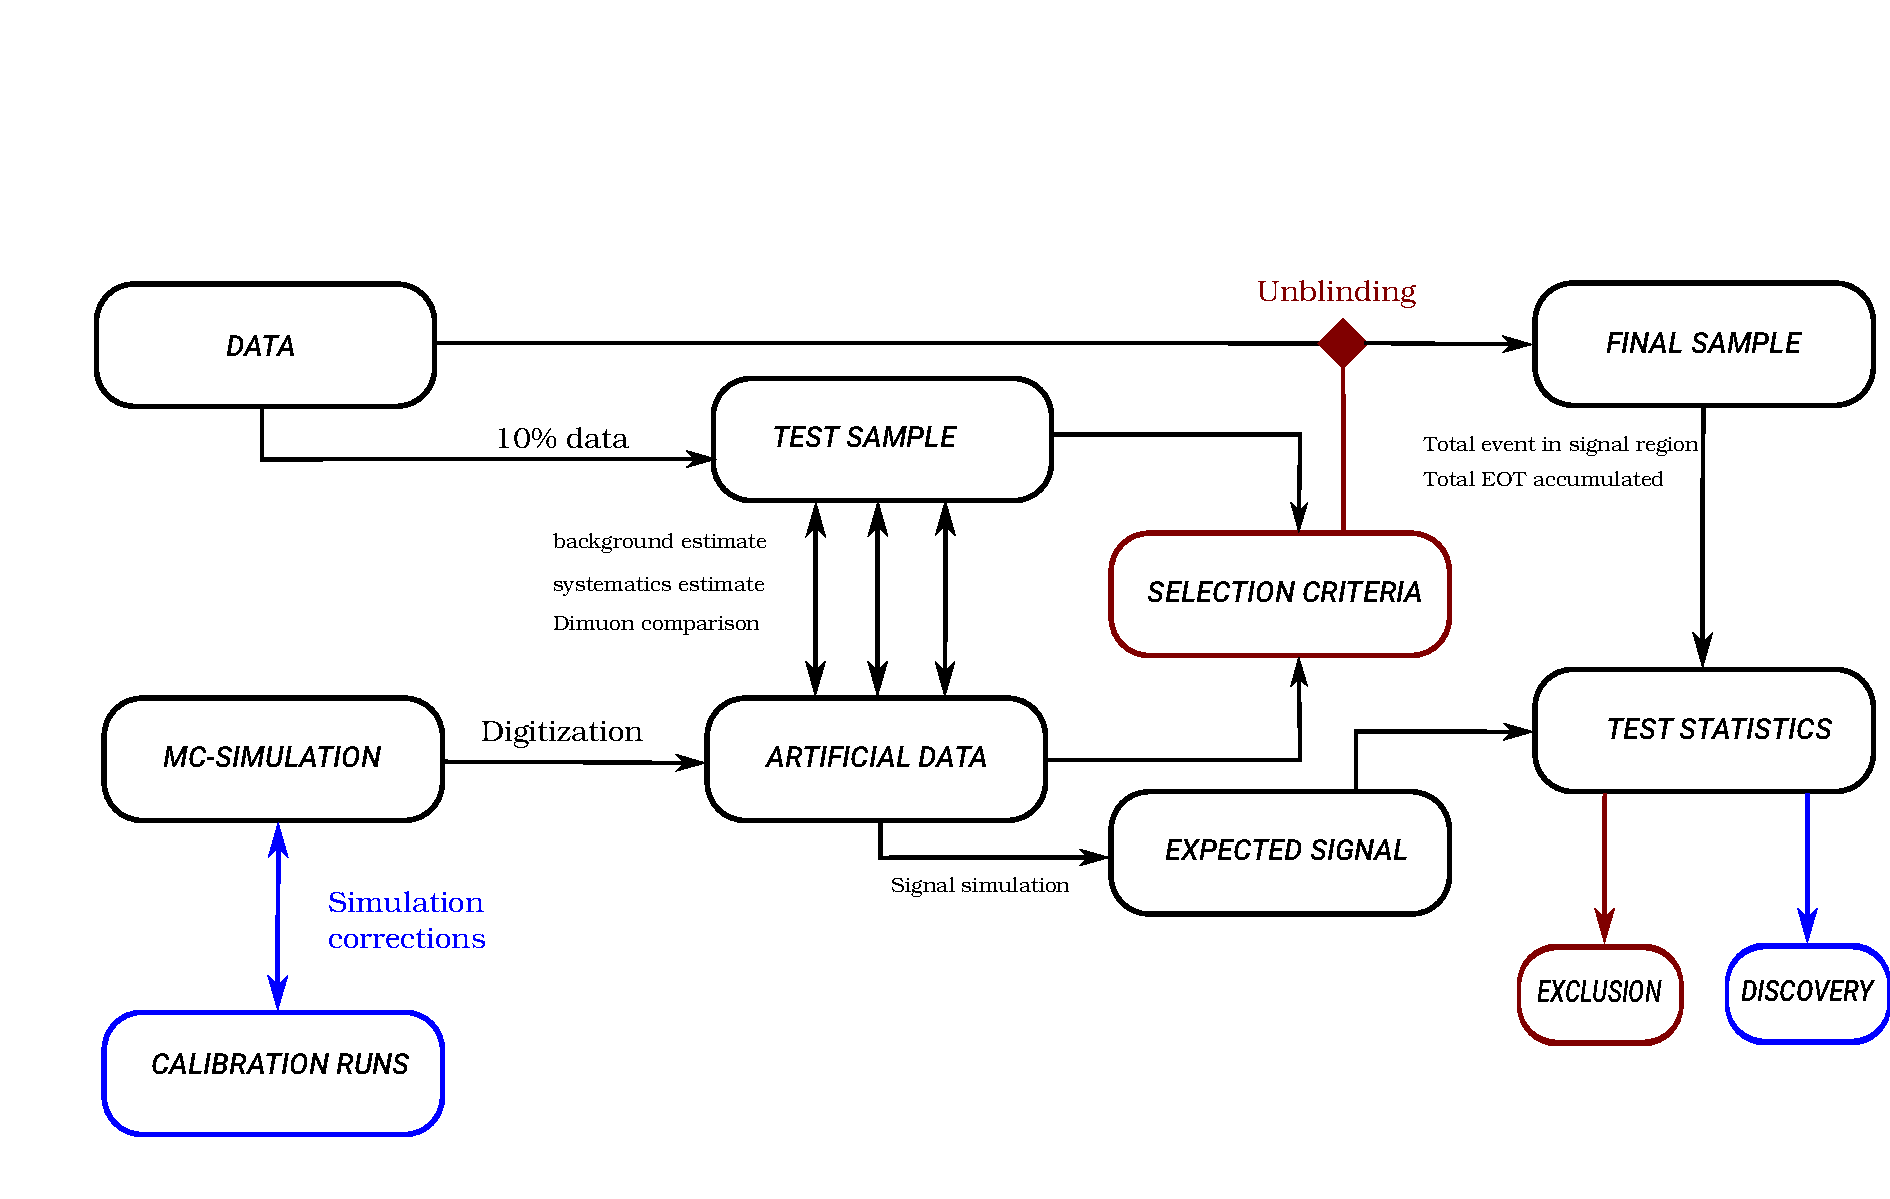
\includegraphics[scale=0.4]{\pdirthree/analysis-chart.pdf}
  \caption{Flowchart of the NA64 analysis.}
  \label{fig:analysis-chart}
\end{figure}

\section{Geant4 simulation of the experiment}
\label{ch3:sec:geant4}

As stressed above, the first ingredient for our analysis is Monte Carlo simulation to reproduce the particle interactions in our complex setup. This task can be divided in three subtasks:

\begin{enumerate}
\item A code to simulate particle interaction inside the NA64 setup.
\item A code to reproduce the detector response in our setup.  
\item A code that describes in detail the properties of $A'$.
\end{enumerate}

The first task is handled by the Geant4 library\cite{AGOSTINELLI2003250}. Geant4 software includes facilities to handle the geometry description, particle tracking and run management. To produce a simulation, the end user must provide an accurate description of the setup, a list of the interactions that need to be simulated, and the phase-space of the primary particle, in terms of particle type\footnote{}, initial particle momentum and initial particle position.

The setup is described using different C++ classes to detail the precise geometry of each detector (See Tab....). To each geometry, a logical volume is assigned, which details the property of the geometrical object. In most of the cases, this means the Z,A number of the nuclei and the density. These property were taken from the NIST database\cite{nist-database}, unless more reliable information (coming from example from the manufacturer of the detector) were found. In some cases, for example to describe the vacuum and the gas detectors, pressure and temperature are also described using in-situ measurements. Finally, detectors are placed in the simulation following the measurement made with a tape (with precision of approximately 1-2 mm). For the trackers, which are particularly sensitive to their exact positioning, an additional measurement was performed by the H4 team with a precision of 0.5 \mmi\cite{meterology-measurements} and later corrected with an alignment procedure performed by the CORAL software\cite{ABBON2007455}.

A physics list is then provided to simulate the relevant physics in the virtual setup. The physics list used in the simulation is the \textit{FTFP BERT} modular physics list, which is recommended for high energy physics experiment \cite{ALLISON2016186}. This physics list combines an excellent description of electromagnetic physics and a description of the inelastic hadron-nucleus processes based on the Fritiof Parton Model (FTF) \cite{Uzhinsky:2013hea}, Bertini intranuclear cascade \cite{Heikkinen:2003sc} and Precompound models \cite{Apostolakis:2009zz}. Because of the complexity of these models and the absence of a solid theory of QCD at low energy, the description of the inelastic scattering for hadrons can still be problematic and a cause of systematic in the experiment. As we will see in Sec.\ref{ch3:sec:geant4-hcal-corr} this problem is addressed by correcting the model using data from calibration run. Following the prescription at the beginning of this chapter.

The last problem is too add the $\DM$ physics description to Geant4. This is currently done by an additional code that describes Dark Matter in a modular way following Object Oriented style of C++. This allows for the description of many Dark Matter candidates inside the same framework. The code has the following functions:

\begin{enumerate}
\item Compute the total cross section of $\DM$ emission as function of the properties of the target nucleus (namely Z, A and density $\rho$) and the primary energy.
\item Decide if the emission of $\DM$ is happening inside a specific Geant4 step by throwing a random number.
\item Sample the final state energy and angle based on the information of the primaries.
\item Compute the decay time in the laboratory system if the model predicts a visible decay and pass the information to Geant4.
\end{enumerate}

An instance of the Dark Matter class is called at the start of each run performed by Geant4, initialized with specific parameters of $\epsilon$ and $m_{\DM}$. The method of the class are then called at each step involving an $e^-$/$e^+$ (or an $\mu^-$/$\mu^+$ for the muon mode) to calculate the total cross section and to decide if an emission is performed. After that, energy and angle are sampled using a distribution $E_{\DM}(E_{e^-}, \theta_{\DM})$. In the case of the invisible mode, the energy of $\DM$ is subtracted to the particle who emitted it and its momentum recalculated. No new particle is created inside the simulation, as the NA64 experiment assumes no further interaction of the decay product $\dmchi$. In the case of the visible mode, the decay length of $\DM$ is computed as function of its energy and parameter, and an $\ee$ pair is created inside the decay volume by sampling the corresponding decay distribution in that region. A weight corresponding to the probability of $\DM$ to decay inside the decay volume (which is simply the normalized integral of the decay distribution along the decay volume) is saved as meta-information of the event, and later used to correct the signal yield.
The initial differential cross-section and precise energy spectrum of $\DM$ was initially calculated using the IWW-approximation. Currently this estimate was improved using a complete tree-level calculation of the cross section \cite{DMsimulation}. This correction decreased the expected signal yield for mass larger than 10 MeV, but decreased it for mass smaller than 5 MeV significantly. Finally, a biasing system was added to the code to increase the cross section artificially. This is required to simulate efficiently the signal without the need of extremely large simulations. A correction factor $N_{norm}(\epsilon_{bias},m_{\DM})$ is calculated by the code and saved as metadata in the output of the simulation. The number of $\DM$ simulated scales linearly with $N_{norm}$, allowing a quick correction for the signal yield in the simulation. The most relevant number for this is the expected number of $\DM$ produced normalized for the total EOT, which we will call $\dmpereot$. This can be calculated simply from the output of the simulation using the following equation:

\begin{equation}
  \label{eq:1}
  \dmpereot = \frac{N_{norm}}{N^{tot}_{sim}} \times \sum^{n=N}_{i=0} \omega_i
\end{equation}

Where $N^{tot}_{sim}$ are the total number of events simulated, and $\omega_i$ is the weight associated to an event. For an event without $\DM$ production or that did not passed the selection criteria, this is weight is zero. Else, this weight can assume a value between 0 and 1, which is corresponding to the probability of $\DM$ to decay in the fiducial volume. Obviously in the case of an invisible decay, the number is always 1, since a missing energy will always be visible if the events pass all selection criteria. For the case of the visible mode on the other, the number to the probability of $\DM$ to decay inside the fiducial volume mentioned above.

The output of the simulation is a text file containing all relevant information that can be used for later analysis. This will be explored more in detail in Sec.\ref{ch3:sec:geant4-digitization}.

The final ingredient to start the simulation is an input particle to trigger the whole machinery. This is done using electron and hadron calibration run to extract a reliable beam profile. As mentioned, the hadron and electron beam are quite different from each other (as it turns out, this feature can also be used to cross check the contamination of each of them). For the case of hadrons, the beam is parametrized as an ellipse, with total width in X direction of 14.5 \mmi and 6 \mmi. In the case of electrons, the parameterization use a 2D Gaussian distribution with $\sigma_x$=4.13 \mmi and $\sigma_y$=1.4 \mmi. In both cases, the entrance angle of the particle is assumed to be uncorrelated from its initial position, as is parametrized with a Gaussian of width $\sigma_r$=0.4 \mrad. These parameters were obtained by fitting the core of the distribution with a Gaussian in both these projections. The fit was performed using two different Micromegas and agreed within 5\% error. 

\subsection{Correction of longitudinal shower profile in the Hadronic calorimeter}
\label{ch3:sec:geant4-hcal-corr}

One instance of the effect that must be corrected inside the MC simulation is the precise energy deposited inside a calorimeter as a consequence of a intranuclear inelastic scattering in the converter. Since we know the majority of particles inside the calibration beam are $\pi^-$, we can do a first degree comparison by simulating a suitable sample of this particle and compare the distribution with what we measure in a calibration beam. The results of this first comparison is shown in Fig.\ref{fig:ecal-comp}. In the first plot we see the comparison of energy deposited in the WCAL for electrons measured in the calibration run compared to what measured in the simulation. As expected because of the QED nature of the process, the two distribution agrees quite well in the core, with some minor disagreement in the tail mostly due to pileup. Here we notice as well that the width of the distribution is roughly. On the other hand, even account for detector correction, we can see that there is a fundamental disagreement at the end of the spectrum when the comparison is performed with pions, specifically in the region relevant for deep inelastic scattering. One could of course suspect some electron contamination given the position of the tail, however the data are first filter by requiring at least 5 MeV energy deposited in both SRD counters facing the beam inlet. This reduces the contamination conservatively at a level $<$0.1\%, which is far below the disagreement observed. A faulty calibration is also unrealistic, since the agreement with electrons is excellent in that energy range. It would look like the simulation systematically overestimate the number of events in that region, where most of the energy released in the inelastic scattering is emitted in the form of $\pi^0$, hence producing a large energy deposit.

\begin{figure}[bth!]
  \centering
  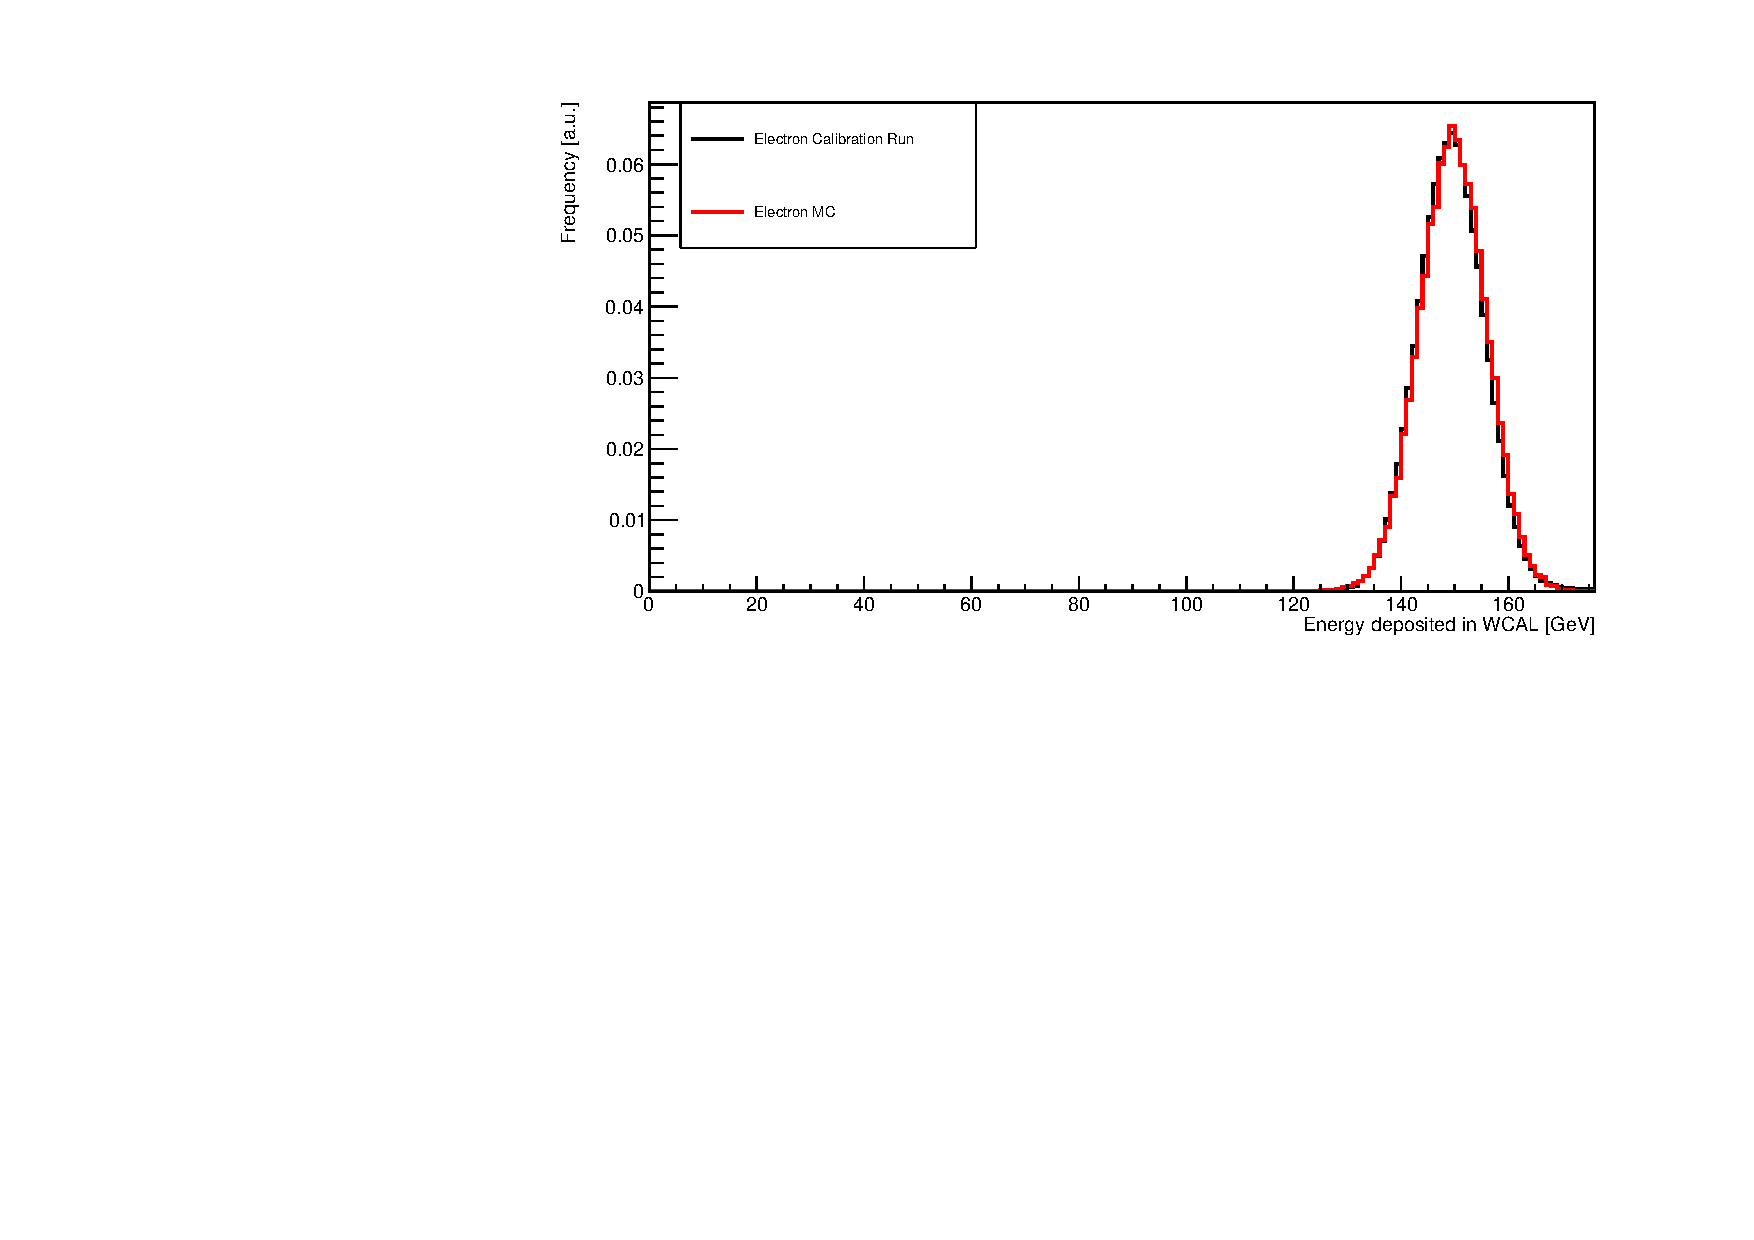
\includegraphics[scale=0.6]{\pdirthree/wcal_elec_comp.pdf}
  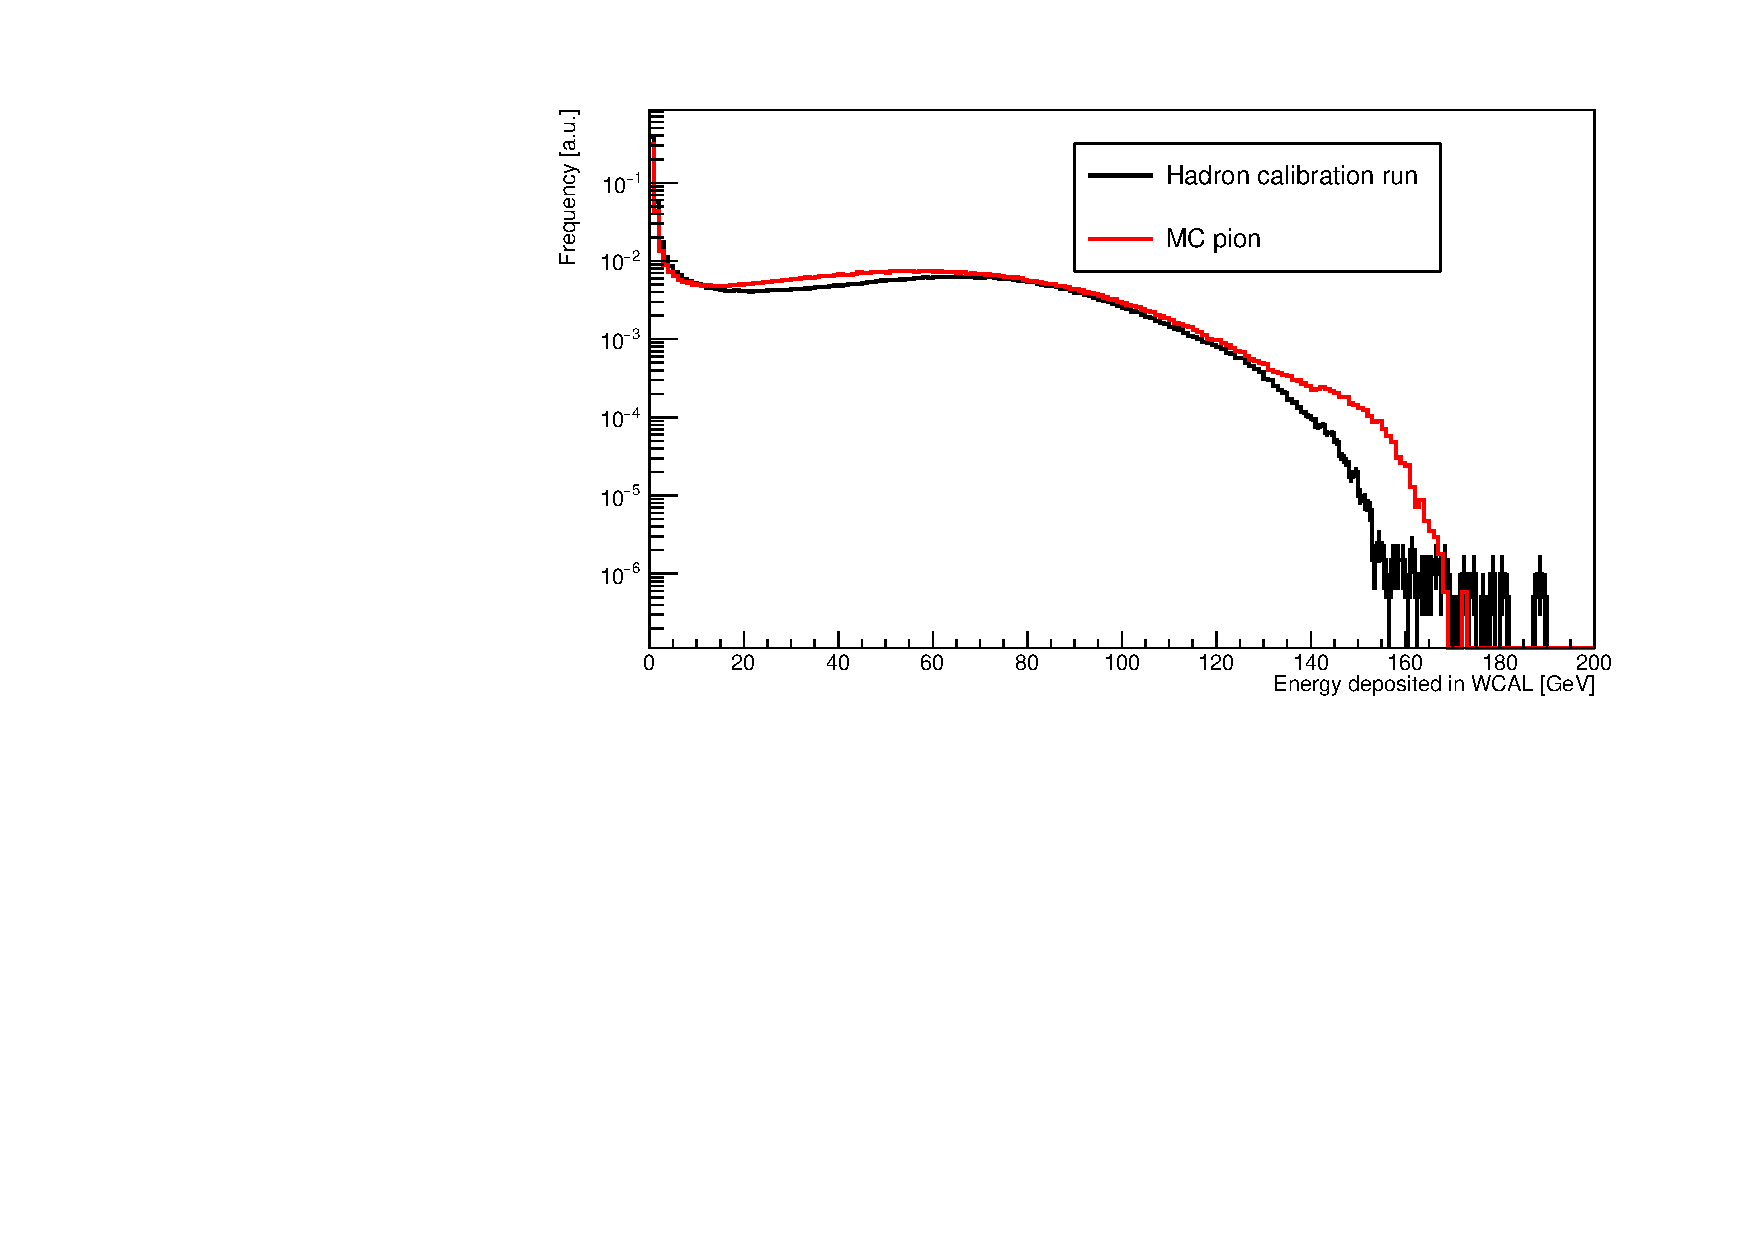
\includegraphics[scale=0.6]{\pdirthree/wcal_pion_comp.pdf}
  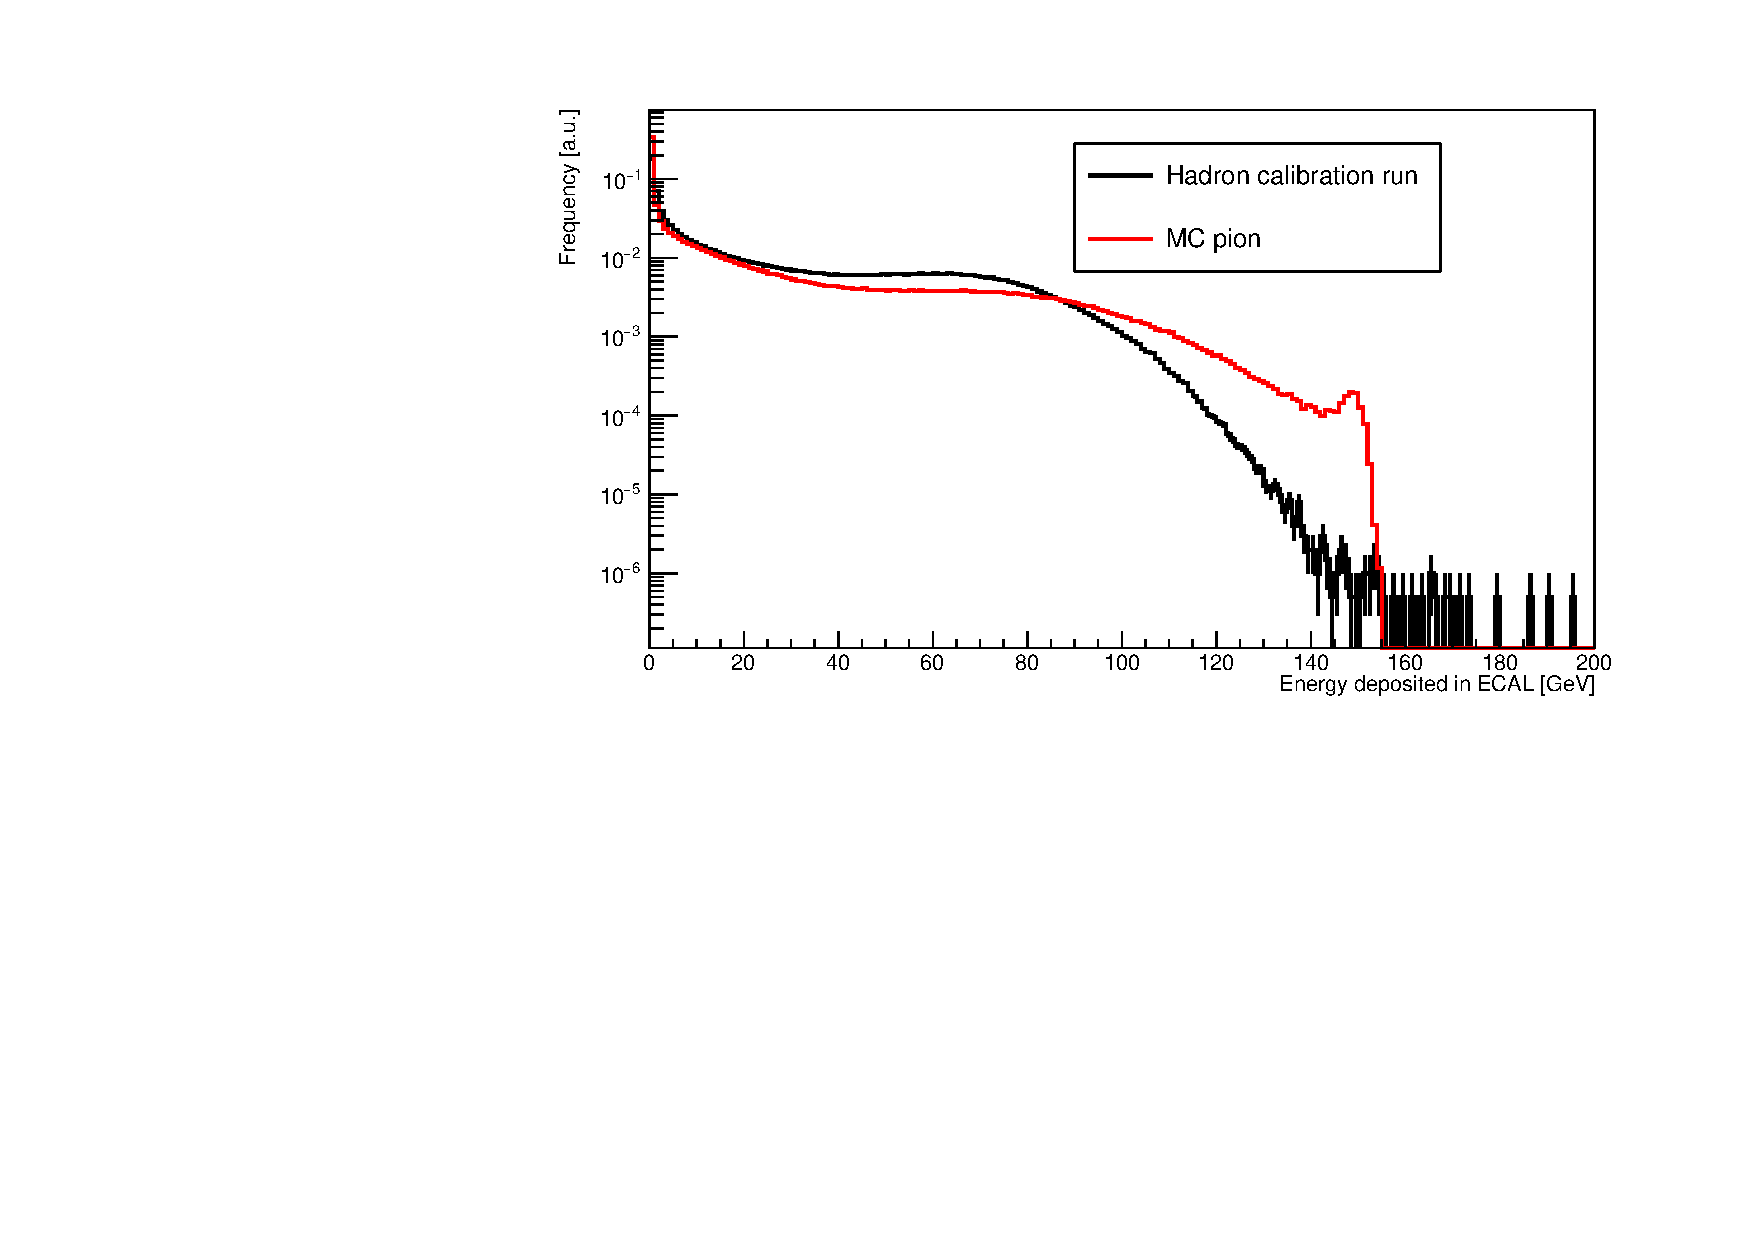
\includegraphics[scale=0.6]{\pdirthree/ecal_pion_comp.pdf}
  \caption[MC/DATA Comparison of $\pi^-$ in ECAL and WCAL]{Comparison between MC and data for different detectors and different runs. Top: WCAL energy deposited for electrons, Middle: WCAL energy deposited for hadrons, Bottom: ECAL energy deposited for hadrons.}
  \label{fig:ecal-comp}
\end{figure}

The same comparison was also repeated for different particle species to cross check the divergency in the beam.

\subsection{Output digitization}
\label{ch3:sec:geant4-digitization}

The output of Geant4 can be divided in three different categories:

\begin{itemize}
\item Energy deposited in the active area of a detector readout by the DAQ.
\item Hit information of a particle passing through the active area of a tracking chamber.
\item MC truth information regarding the event, including all the kinematics of the $\DM$ in the case it was emitted.
\end{itemize}

The first type is straight forward. Each time a step happens inside a sensitive detector, the energy deposited in the volume is added to some specific counters which are in the end outputted into the end file. At this point the energy is mostly computed starting from physical effect, but some detector effected are already accounted for. Most notably, only the energy in the active part of each calorimeters (ECAL, WCAL and HCAL) is recorded, and the total sum of the energy deposited is corrected using a calibration constant which corrects the energy output to reflect the initial particle energy. Additionally, Birks law \cite{NYIBULE2014141} is implemented in the HCAL to correct for the propagation of optical photon in the WLS until the PMTs, using an attenuation length of 30 \si{\centi\meter}. This effects correct for the different light yield between $\pi^-$ and $\mu^-$, since in the case of $\mu^-$ the energy is deposited the full length of the detector evenly.

To reproduce tracking detectors, every time a particle cross the gas volume of a gas chamber, multiple information are saved:

\begin{itemize}
\item x-y-z position of the particle at the beginning of the step.
\item The energy of the particle responsible for the hit.  
\item The energy deposited in the gas during the step.
\item The PDG number of the particle \cite{particle-numbering-scheme}.
\end{itemize}

These data define a structure called MChit, which is later used by the reconstruction algorithm to reproduces hit in the same format of the data. The algorithm for the reconstruction works as follow: first, only hits with a minimal energy deposit in the volume are considered, since a minimum amount of energy need to be deposited to start the ionization inside the volumes. Practically, the minimum threshold was assumed to be 2 keV based on previous studies performed for MM \cite{IGUAZ20121079}. A similar value is assumed for GEM detector as well. After that, multiple MChit are merged if they are found to be closer than a certain distance. This distance is conservatively set to be 2 \mmi for MM and 1.75 mm \mmi for GEM (see Sec.\ref{ch5:sec:separ-hit-micr}). Hit closer than distance are merged in a single one and the new x-y position are computed by weighting each position by its energy deposit in the gas. Starting from here, the xy coordinates of the hits are transformed into the plane of the detectors using a simple matrix multiplication $u_{hit} = M_{uv}(\theta_{uv}) \cdot v_{hit}$ where $u_{hit}$ is the hit position in the detector coordinate system and $v_{hit}$ is the same vector expressed in the laboratory system. The Matrix $M_{uv}(\theta_{uv}$ is the rotation matrix of the $O(2)$ group where $\theta_{uv}$ is the angle between the two axis of the detector and the axis of the laboratory system. From here, knowledge of the original hit is no longer assumed, and each coordinate on the detector plane is treated separately. This is necessary to reproduce faithfully the detector condition, indeed the experimentalist get this information from each plane separately, hence in the end it will end up with a set $X_n$ and $Y_n$ of XY position that he will need to combine to create the hit candidates\footnote{In the most common case of just a single primary present upstream the ECAL, of course this association is trivial. Since only one hit per plane is present}. In the MM detector, the clusterization is fully reproduced, the physical cluster is parametrized by a simple Gaussian, and charge is distributed on the phjysical strips starting from the center of the hit (computed in the step before). Each charge is then smeared with a Poisson distribution to reproduce charge fluctuation in each channel. The total charge of the cluster is decided starting from the total energy deposit in the gas volume and converting it into charge based on a simple calibration procedure using the data of the electron calibration runs. Since MM is a multiplexed detector, no direct information of the strip is directly accessible. The physical strip are now mapped to the corresponding channel, and a 64-dimension vector is obtained as output. Noise is also added to each channel using the same pedestal measured in the sparse mode of the APV chips. Now that each channel charge is defined, the vector is used as input for the same clusterization procedure used for the data, which ultimately returns each cluster candidates and calculates the most probable position as the weighted average of all the strips in each cluster. The procedure for the GEM is more direct and only involves the smearing of the initial true hit position using a Gaussian distribution with width corresponding to the hit resolution of the GEM detectors, estimated from calibration data using the Three Layer Method \cite{Bortfeldt:2014vvt}. This determined a resolution of $\sigma_{GEM} \approx 80$\mum. Either way, after the set $X_n$ and $Y_n$ is computed, the new set of hit candidate $hit_n$ is formed with all possible combination of each set. Thankfully a hit number per plane larger than five, other than being very rare ($\lesssim$1\%), is not relevant for $\DM$ searches and hence rejected during the analysis. The hits candidates are then used as input of the tracking or vertexing procedure. The tracking procedure is straight forward and described in detail in \cite{dbanerjee-thesis}, the total momentum of a track is calculated from the displacement after passing through the magnetic field of the MBPL.



The vertex reconstruction is more involved but starts from the same input above. The procedure will be described more in detail in Sec.\ref{ch3:sec:vis-mode-tracking}.

\subsection{Signal simulation}
\label{ch3:sec:geant4-signal}

\section{Background}
\label{ch3:sec:bkg}

In this section, we will try to go more in detail of what constitutes background in the NA64 experiment. First of all, with background we mean obviously an event that is detected is the signal region without involving the emission of $\DM$, and that was able to pass all our selection criteria. Because of the different physics involving them, it is instructive to divide the background by the primary particle considered. This gives us three category:

\begin{description}[leftmargin=!,labelwidth=\widthof{\bfseries Electronic background}]
\item[Hadronic background] Background coming from an hadronic primary.
\item[Muonic background] Background coming from a $\mu^-$ primary.
\item[Electronic background] Background coming from a $e^-$ primary.
\end{description}

This classification is convenient, especially if one wants to study the background using MC-simulation (as what will be relevant for the simulation is the primary particle). However, there is some overlap in the physics of these three scenario, and we need to remind ourselves that sometimes the same type of background can arise from different sources. A trivial example would be the decay $\pi^- \rightarrow \mu^-\nu$, where an initial $\pi^-$ produces a $\mu^-$ in our setup. A more relevant but involved example is an $e^-$ or a $\gamma$ which trigger an hadronic shower after an inelastic scattering with a nucleus. This can potentially cause energy escaping in the form of hadron, and since the initial particle is an electron, such background is also accepted by the SRD criteria. The main advantage of this classification is that it let us calculated the suppression factor for the background with simple argument without necessarily using the MC-simulation. For example, for both hadronic and muonic background, we can conservatively assume a factor $10^{-5}$/EOT\footnote{As seen in Sec.\ref{ch3:sec:bkg-srd} the suppression is typically larger,} of suppression due to both their low concentration in the beam and the SRD selection applied upstream, which is almost always independent from the precise physics of the background studied.

\subsection{Invisible mode background}
\label{ch3:sec:bkg:inv}

\subsubsection{Hadronic background}
\label{ch3:sec:bkg:inv:hadr}

In the case of invisible mode, the \textbf{Hadronic background} can arise simply from a $\pi^-$ that after leaving a minimal energy in the ECAL punch-through the HCAL undetected. In first approximation using an interaction length of 21 $\lambda_{int}$ this can be calculated to be $\lesssim 10^{-9}$. This without accounting for the high efficiency VETO after the ECAL, SRD rejection, and the fact that the HCAL is able to detected a MIP interaction even without an inelastic interaction happening. Each of this factor push the background well below $<10^{-13}$ as pointed out in the NA64 first proposal \cite{Andreas:2013lya}. A more relevant background would be an hadron scatter inelastically inside the ECAL in a process:

\begin{equation}
  \label{eq:pion-nucleus-scattering}
  h + Z \longrightarrow h + Z + hadrons)
\end{equation}

In this process, part of the energy can evaporate as consequence of some particles emitted at large angle and thus escaping the setup in the direction transverse to the beam. This reaction is typically suppressed by shower profile analysis, energy deposited in the pre-shower, and the presence of a VETO at the end of the ECAL. The phase space of this process is however very complicate, and a lot of possible phenomenology can arise from it. For example, large energy deposited in the pre-shower can be a simple consequence of some $\pi^0$ backscattering after the hadronization, while the shower profile can mimic the one of the electron if a large fraction of energy in the inelastic scattering is carried away by $\pi^0$. Also, if particles are emitted in the form of neutrons or other neutrals (for example ...), the VETO would be ineffective to reject them. To have a crude estimate, we can take the process \ref{eq:pion-nucleus-scattering} and assume $\geq$2 neutrals particles are produced as consequence of the hadronization. This gives us a probability equal to \cite{gkkk1}:

\begin{equation}
  \label{eq:transverse-leak-estimate}
  P \simeq P_n \cdot P_{la} \cdot P_{leak}
\end{equation}

Where we define $P_n$ the probability of such interaction to occur, $P_{la}$ the probability to produce particles at large angle of scattering, and $P_{leak}$ the probability to escape HCAL without interactions. Here we stress again that this formula hides a large number of topologies that such event could have, however plus in some number can be instructive to get an intuition for these processes. Since the ECAL has $\lambda_{int} \simeq 0.5$, the probability of interaction for an hadron is fairly high (roughly 50\% of the time such interaction will happen). We need at least 50 \gev of energy leaking to produce a signal event, if we assume two neutrals to be produced at $\Theta_{n} \simeq 30$\si{\degree} this would mean crossing at least 4$\lambda_{int}$ each, for a $P_{leak} \lesssim 3 \cdot 10^{-4}$. We can take the measured values of the NOMAD to estimate the value of the cross section in this range \cite{AUTIERO1998285,GNINENKO1998583}. The probability of separating a cluster with energy $>$0.1E$_{\pi}$ at an angle $\Theta_{n} \gtrsim 30$\si{\degree} was measured to be P$_{la} \simeq 10^{-5}$ and drops very quickly wit the beam energy, as shows the fact that a factor 20 difference was found between 15 \gev and 6 \gev $\pi^-$. Even taking the value this (very) conservative value as $P_{la}$, we see that the probability of the energy escape is already $P\simeq 10^{-9}$, which multiplied to the hadron contamination and SRD suppression leads to an estimate of $P<10^{-14}$ for this background. Another possible background is the decay of hadron inside the setup in neutrinos, which would ultimately lead to evaporated energy. The high energy of the primary suppress this background, since at 100 GeV the chance for a $\pi^-/K^-$ to decay is $P^{decay}_{\pi} \simeq  10^{-2}$\footnote{calculated for a total length of 20 m assuming light-speed.}. There are multiple possible decay that are accompanied by a neutrino emission, the most likely one being the $\pi^-$ decay $\pi^- \rightarrow mu^- \nu_{\mu}$. The emission of the muon makes such decay very easy to spot, since it will an energy deposit both in the VETO and the HCAL, for a total probability similar to the one of a punchthrough $\pi^-$ ($P < 10^{-14}$). One could argue that the $\mu^-$ could decay: $\mu^- \rightarrow e^- + \nu_{mu}+ \hbar{\nu_{e}}$, producing an electronmagnetic shower with missing energy. The long decay time of the $\mu^-$ adds however an additional suppression factor of $P\simeq 10^{-5}$, which together with the upstream selection criteria put the background conservatively at $P \lesssim 10^{-13}$. Interesting is the case of $K^-$, which posses a pure electromagnetic channel of decay with missing energy in the form of an emitted neutrinos: $K^- \rightarrow \pi^0 + e^- + \hbar{\nu_e}$, commonly called $K^-_{3e}$, with a branching ratio of $\Gamma_i/\Gamma_{tot} \approx$0.05 \cite{particle-strange-mesons}. The total probability of background for an incoming $K^-$ is around $P\simeq 10^{-3}$ accounting for both probability of decay and branching ratio. A MC-simulation of $K^-$ confirm this simple estimate as shown in Fig.\ref{fig:kaonbkg-sim}, where the fraction of event in the signal region correspond to the probability calculated. Multiplying this probability for the SRD selection criteria and the suppression from the beam returns a probability of $P_{K_{3e}} < 10^{-12}$\footnote{Here a suppression from the beam of 10$^{-3}$ is used, since the the $K^-$ is a smaller fraction than the contamination \cite{h4-beamline}}. This start to be significant and worth of precise study. It turns out that there are additional factor of rejection for this background, coming mostly from a more precise account of SRD in this scenario and some small effect from other cuts (tracking, shower profile, etc...) the expected background is $P_{K_{3e}} \simeq 10^{-13}$.


\begin{figure}[bth!]
  \centering
  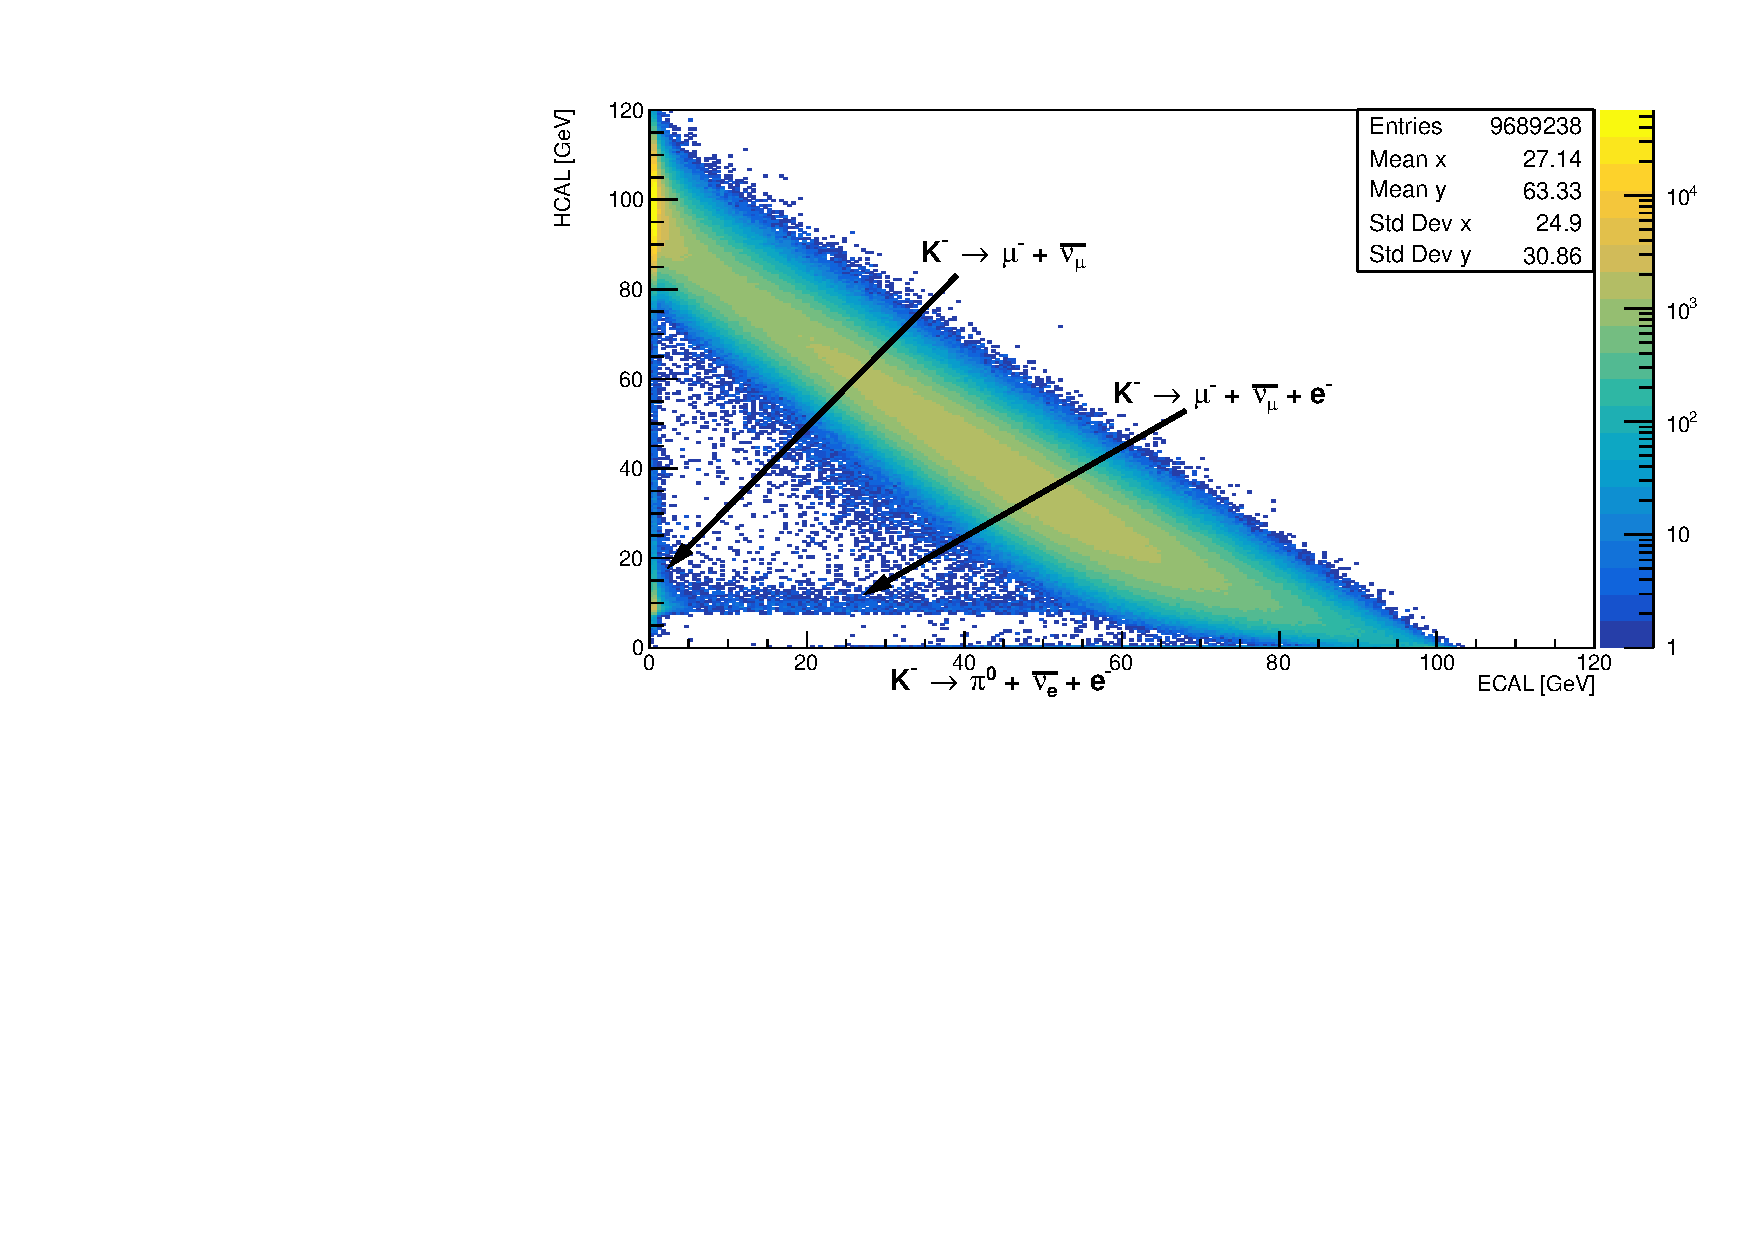
\includegraphics[width=\textwidth]{\pdirthree/kaonbkg.pdf}
  \caption[$K^-$ simulation ]{Energy deposited in the ECAL vs energy deposited in the HCAL after simulating $K^-$ as primary particle in the NA64 setup. The number of event inside the signal box}
  \label{fig:kaonbkg-sim}
\end{figure}

\subsubsection{Muonic background}
\label{ch3:sec:bkg:inv:muon}

The second type of background is the background coming from a muon primary. This type of background is also largely suppressed by both beam composition and SRD selection criteria, to a level of approximately $10^{-7}/EOT$\footnote{Also here the suppression from the beam composition is larger \cite{h4-beamline} and SRD selection criteria are more stringent.}. As in the case of $\pi^-$, we can convince ourselves that a complete punchthrough of the setup without being detected is negligible. Indeed the muon need to travel through both the VETO and 3HCAL without leaving any detectable energy deposit. Using $\lesssim 10^{-3}$ for leaving an undetectable energy in the VETO and $\lesssim 10^{-4}$ to deposit less energy than the threshold in all modules, we see that the background is conservatively $< 10^{-14}$. In the case of muons, the nuclear interaction are largely suppressed, hence there is no chance for a large amount of energy to escape transversely. What remains is the decay $\mu^- \rightarrow e\nu\nu$, which could create neutrinos. We remind ourselves here that the large decay time of $\mu^-$ add an additional suppression of $\lesssim 10^{-5}$. Here again proper accounting of SRD and misalignment of the $e^-$ accounting for an additional $P\sim 10^{-1}$ factor, putting this background at a level of $P_{\mu} \lesssim 10^{-13}$.

\subsubsection{Electronic background}
\label{ch3:sec:bkg:inv:elec}

The last type of background is originating from electron primary. This is more tricky, since the beam is primary made of electrons, and SRD are tuned to select them, no upstream suppression factor can be achieved. Simple punchthrough of electron through the whole setup is not possible, since the path is blocked by 3 HCAL modules. Other similar event, with energy losses due to non uniformity and cracks in the ECAL/HCAL were as well studied and found unrealistic \cite{Andreas:2013lya}. Low energy electron are also a potential background, if a primary electron with $E_0 < E_{th}$ arrives to the ECAL it will leave an energy deposit compatible with the signal. Such background is also extremely unlikely. The amount of electron $N(E_e<E_{th})$ in the beam with energy lower than the energy threshold for the signal amounts conservatively to $<10^{-2}$. Such particles are normally deflected by the two MBPL magnet outside the acceptance of the ECAL\footnote{A quick calculation shows that for $E_0$=50 \gev the difference in deviation is about 0.4 \si{\meter}}. The tracking system install in NA64 makes sure that the energy of the incoming particle is always measured with a resolution of $\delta p/p \approx 1\%$, particle with large entrance angle in the magnet can in principle enter in the acceptance of the magnet, but their momentum is reconstructed by observing their displacement in the Micromegas. A dedicated simulation of $10^{10}$ EOT was performed by simulating electron with energy compatible with the signal region. No event was found in the signal region after requiring a reconstructed momentum within 3$\sigma$. This allow us to put this background conservatively at a level of $< 10^{-12}$.
An important source of background to be considered is the dimuon production inside the target. As mentioned, these events are very useful to check for sistematics and validated the MC. However, fluctuation in the energy deposited in the HCAL might reach the signal region when significant. The background was estimated by exponential extrapolation of the control sample inside the signal region considering the side band I shown in the Fig.\ref{fig:ehcal-bkg-bands}. This estimate was performed using the control sample without applying the VETO cut, to make the extrapolation meaningful. The cut effect is then taken into account as a factor $\sim 10^{-6}$ as probability of the energy deposited by two MIP two be smaller than $E<E^{min}_{th}$.

\begin{figure}[bth!]
  \centering
  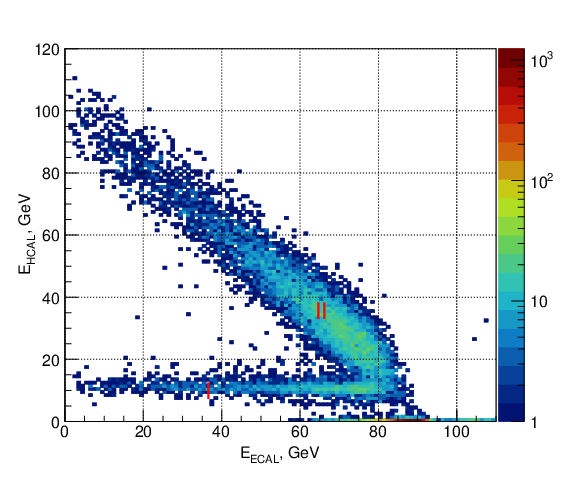
\includegraphics[width=0.45\textwidth]{\pdirthree/EHCAL_lastpub_left.png}
  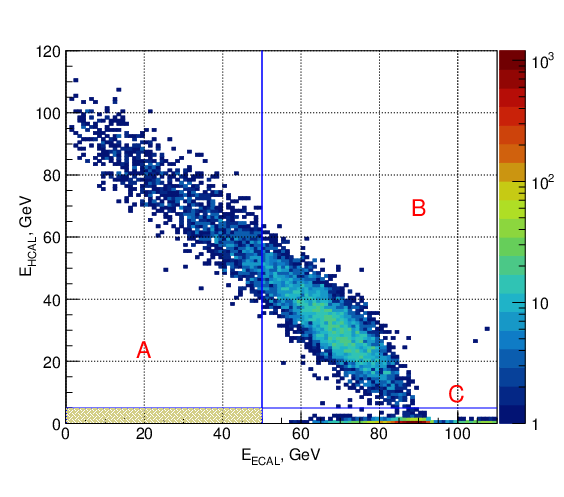
\includegraphics[width=0.45\textwidth]{\pdirthree/EHCAL_lastpub_right.png}
  \caption[ECAL vs HCAL events band]{Distribution of events in the $\ehcalplane$ plane for the control sample of the data. The right panel shows the sample with all the selection criteria. Left panel shows the same sample without the VETO cut. The shaded area is the signal box. The size of the signal box is increased by a factor 5 in the Y-axis direction for illustration purposes. The region labeled I contains event caused by dimuon production, while region II contains mostly event leaking from the ECAL into the HCAL. the side bands A and C are used to estimate the background inside the signal region \cite{NA64:2019imj}.}
  \label{fig:ehcal-bkg-bands}
\end{figure}

The most important background is finally the electro-nuclear and photo-nuclear production of neutral hadrons at large angle. This case is similar to the one discussed for hadrons, in this case however suppression due to beam composition and SRD selection criteria are not present. In first approximation, the rarity of such interaction compensate the suppression factor, and account for $P_n \simeq 10^{-6}$ (see Eq.\ref{eq:transverse-leak-estimate}). In practice, the background was extrapolated using an exponential distribution of the type:

\begin{equation}
  \label{eq:bkg-extrapolation}
  \exp{a \cdot E_{ECAL} + b}
\end{equation}

The parameters $a$ and $b$ are fitted using the data in the side band C of the control sample, i.e. events with E$_{HCAL}<1$\gev and $E_{ECAL}>E_{th}$, and then integrated over the signal region. The results of this estimate was then accounted for conservatively in Tab.\ref{tab:inv-bkg}.
The largest source of background however comes from electro-nuclear production happening upstream the target. As Fig.\ref{fig:eh-prod-sketch} shows, if this interaction happen in a detector with a large distance from the ECAL, the displacement of the particle can be large enough to exit the setup transversely. 


\begin{figure}[bth!]
  \centering
  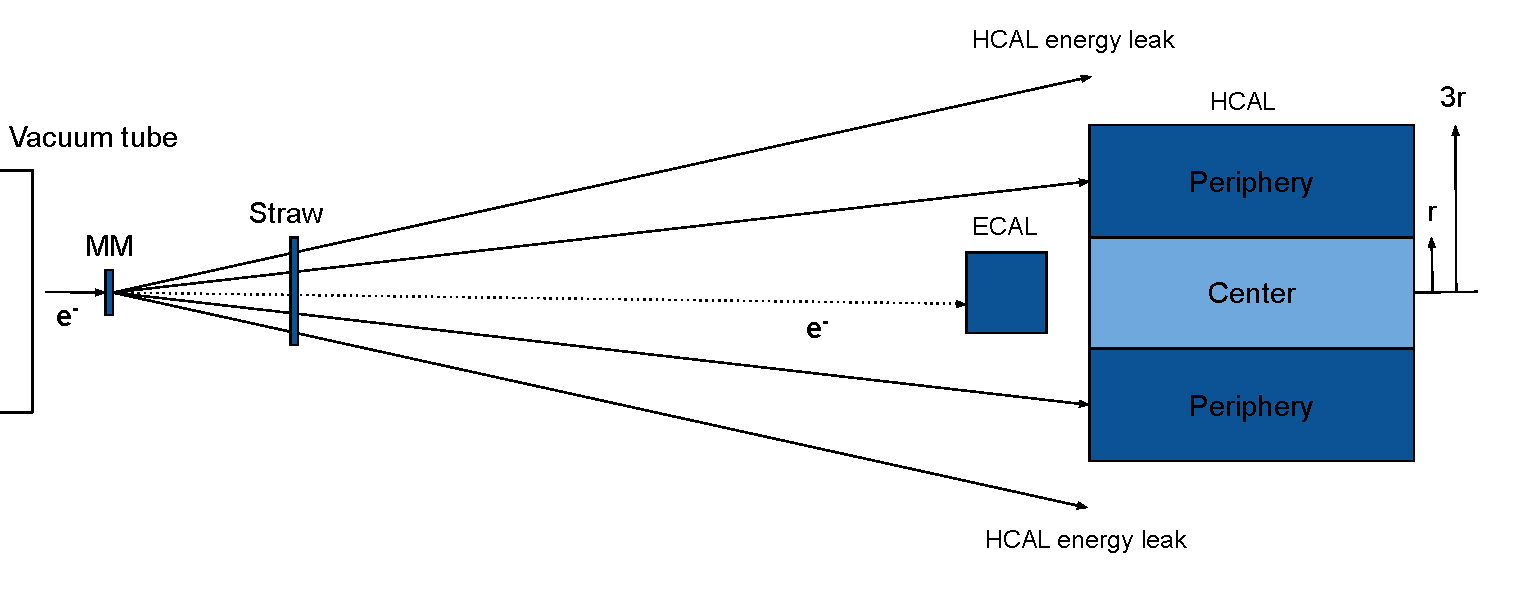
\includegraphics[scale=0.4]{\pdirthree/hcal-leak.pdf}
  \caption[upstream electro-hadron production upstream]{Sketch of electro-nuclear interaction happening upstream the ECAL leading to a possible background \cite{pdegen-thesis}.}
  \label{fig:eh-prod-sketch}
\end{figure}

This background can be estimated by looking at the periphery region of the HCAL. Since the angular distribution is sharply suppressed for large angle \cite{AUTIERO1998285,GNINENKO1998583}, if we assume a distribution coming from large scattering neutral can be a source of background we must see a significant amount of event with low energy deposit in the ECAL and large energy deposit in the periphery of the first HCAL. For this purpose, we define the variable R, defined as ratio between energy deposited in all cell excluded the central one and the total energy deposited in the modules:

\begin{equation}
  \label{eq:R-factor}
  R = \frac{E^{all}_{HCAL} - E^{center}_{HCAL}}{ECAL^{all}_{HCAL}}
\end{equation}

In a normal event with particles leaking the ECAL, we typically observe $R<0.5$, as the HCAL module center is aligned with the beam direction, thus the dominating energy deposit will be in the central cell. If an electro-nuclear production happens upstream however, some distortion of this variable will be visible. In the most extreme scenario when the particle is missing the ECAL completely, the R value can be equal 1, since the central cell of the HCAL will be shielded by the ECAL while the periphery will be directly hit. We can observe such behaviour in Fig.\ref{fig:r-value-csample}: most of the event considered have an R peaked at 0.35. Events where the primary electron loose a large portion of its energy due to bremsstrahlung are shown in region III and are responsable for events with large R value. In this topology of events, the electron completely misses the ECAL after being deflected by the magnetic field, while the hard-$\gamma$ produced in the interaction propagate without deflection and hit the HCAL in the periphery. Such event are also easily identifiable by looking at the HCAL placed in from the original beam direction. In the event of region III, this detector measure energy deposit $E>60$\gev.

\begin{figure}[bth!]
  \centering
  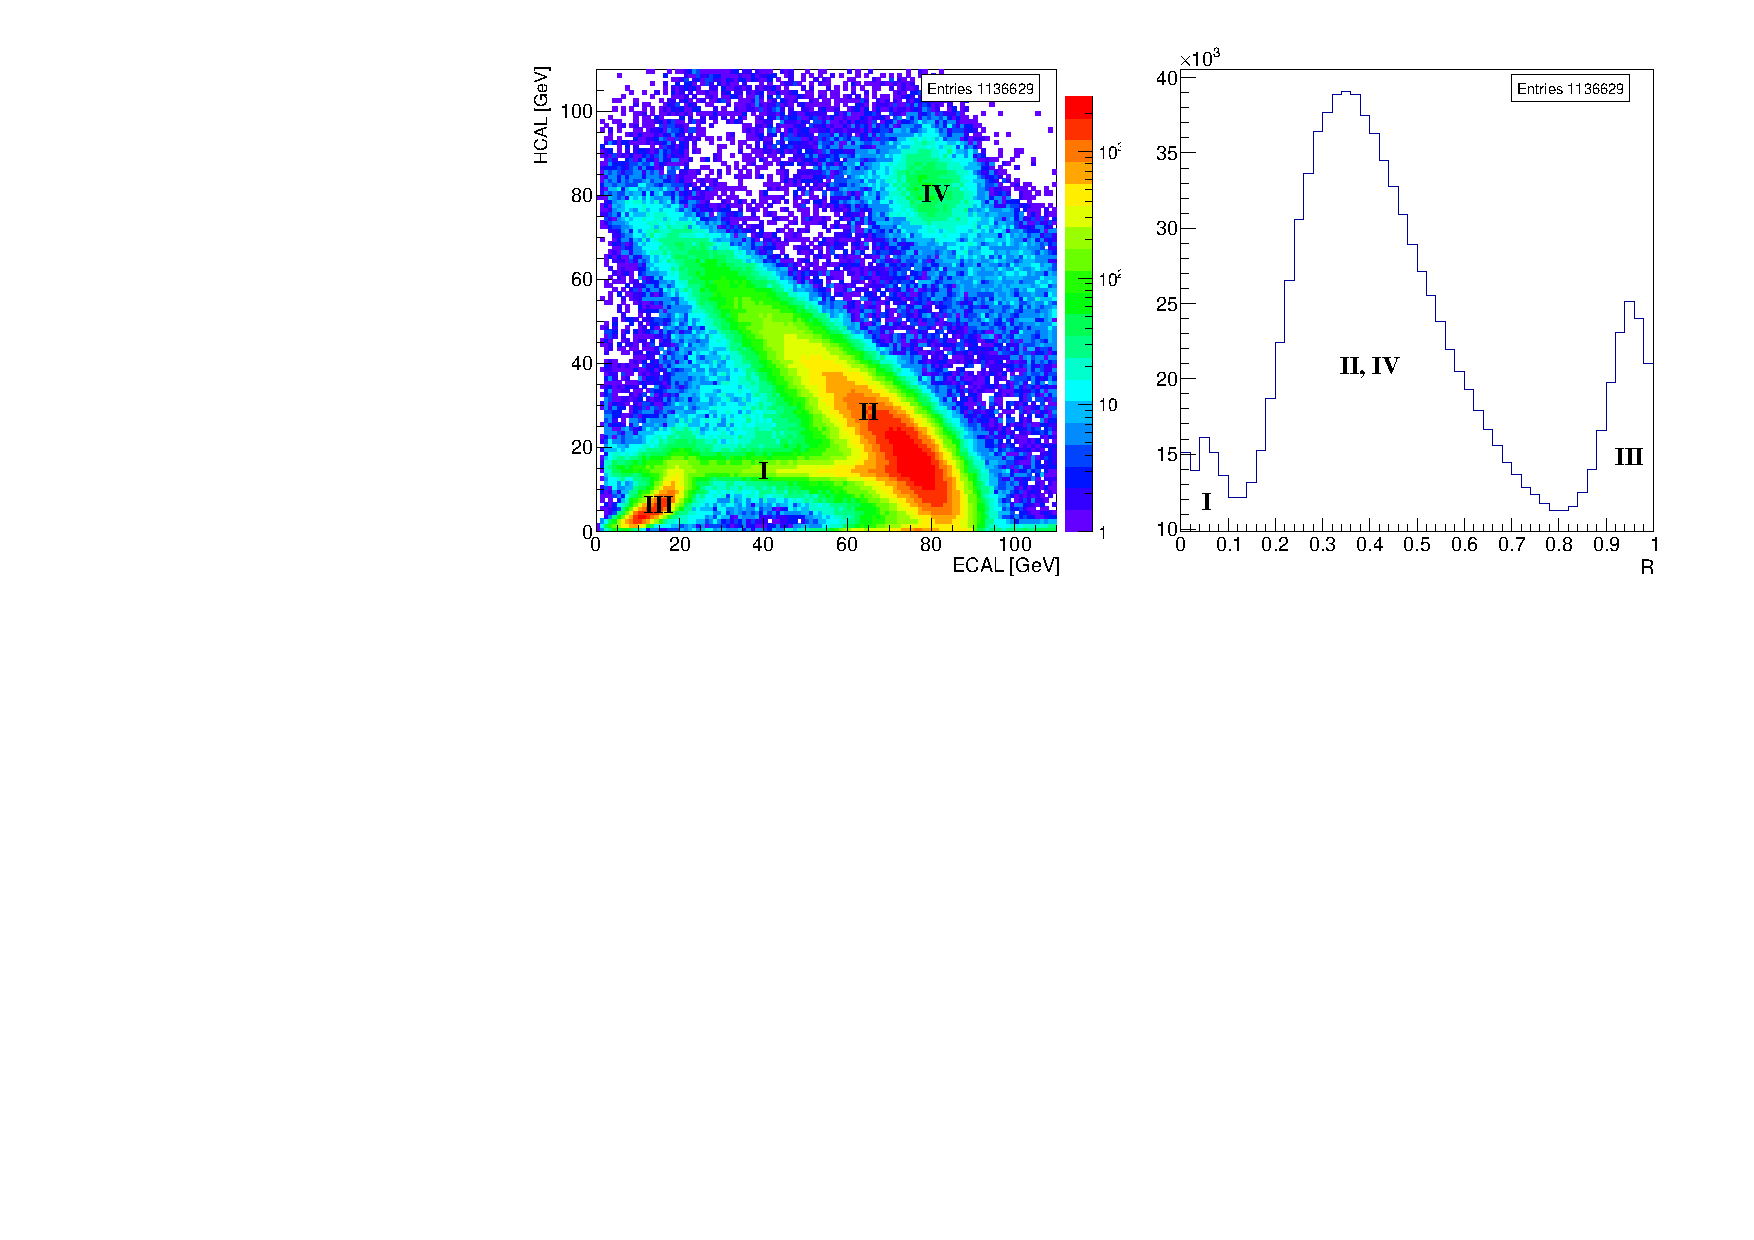
\includegraphics[width=\textwidth]{\pdirthree/pp30-calsr-uncut-may2.pdf}
  \caption[R value for control sample]{Energy distribution in the $\ehcalplane$ (left) and corresponding distribution of the R value for different interesting regions. Region I is populated by the dimuon production inside the ECAL. Region II are event leaking in the HCAL characterized by energy conservation. Region III are event with hard bremstrahlung of the $e^-$ upstream, where the primary completely miss the ECAL and the $\gamma$ energy is deposited in the HCAL perifery. Region IV is characterized by pileup events \cite{pdegen-thesis}.}
  \label{fig:r-value-csample}
\end{figure}

Event with electro-nuclear scattering upstream are characterized by a distribution equivalent to the one of region III. In Fig.\ref{fig:enucl-position} we see the frequency of nuclear interaction for different position along the beamline after the particle exit the vacuum pipe as predicted from a dedicated MC-simulation. Micromegas are the leading contribution to this background, as result of their large budget material, which in terms of interaction length is approximately $\lambda_{int} \simeq 1.9 \times 10^{-3}$. It is noticeable however that a factor $\sim 2$ less electronuclear interaction are happening in the first Micromegas of the beamline. This is the results of the smaller material budget of this module, that uses a mylar windows instead of a cooper top to close the gas box. Reduction of the material budget of the rest of the module will be an important improvement to suppress this background. As the displacement of the hadrons scales with the distance between the interaction and the target, reducing the distance between tracker chamber and the ECAL is also something that will be used for future runs.

\begin{figure}[bth!]
  \centering
  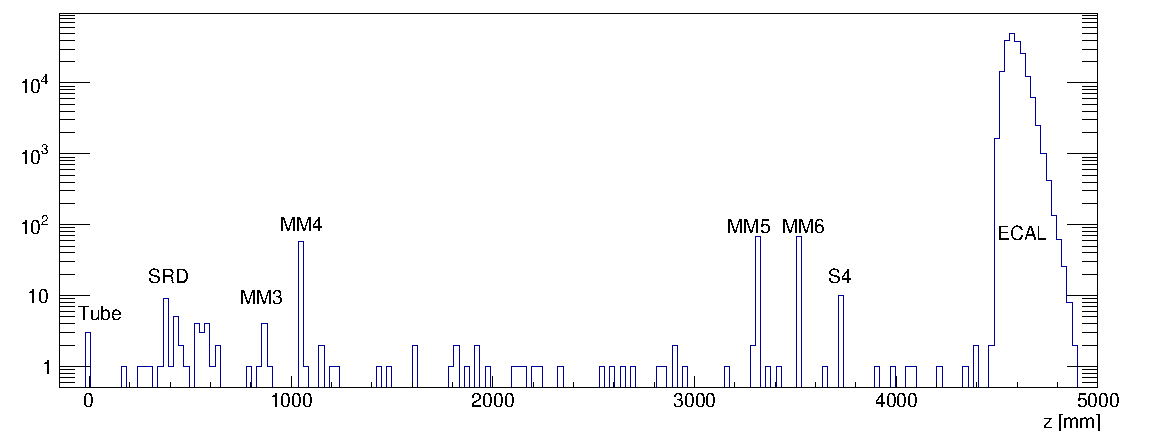
\includegraphics[width=\textwidth]{\pdirthree/enucl-position.pdf}
  \caption[electronuclear interaction position]{Z position of electronuclear interactions between the end of the vacuum tube and the start of the first HCAL. A total of 2.5$\times 10^6$ EOT were simulated for this distribution.}
  \label{fig:enucl-position}
\end{figure}

To properly account for this background, we follow the procedure described in \cite{na64-neutrals-study,pdegen-thesis}, which is reviewed briefly here.


First, we divide the $\ehcalplane$ in 10 different zones as depicted in Fig.\ref{fig:enucl-bkg-estimation}. The zones divide the distribution of observed event in several tile at different distances from the signal region. All the region labeled with even number are events where the energy is conserved and the R value is closer to the one plotted for region II. In the even within zones labeled with odd number on the other hand, some energy is missing from the initial primary electron. The two most relevant are region 7) and 9), that include a portion of the signal region. These events have an R distribution closer to the one depicted in region III, with a sharp peak at 1. To further classify the events in these two regions, we can construct a new category based on the value of the R distribution. We define $n_i(r)$ as the number of events in the region $i$ with distance $r$ from the center of the HCAL. This definition let us build a classification of event useful for the background:

\begin{itemize}
\item $n_{5,7}(r=0)$ is the number of events with any energy deposited in the HCAL.
\item $n_{5,7}(r=r_{cell})$ is the number of events with $R=1$, i.e. no energy is deposited in the central cell of the HCAL.
\item $n_{5,7}(r=3r_{cell})$ are the event with no energy deposited in the HCAL, where R is not defined.
\end{itemize}

The final goal is to calculate the probability of an incoming electron primary to produce an event that fall in one of these categories. Which means computing:

\begin{equation}
  \label{eq:enucl-prob}
  p_i = \frac{n_i(r)}{n_{EOT}}
\end{equation}

In practice, the distribution of $n_{i}(r)$ is fitted using an exponential distribution and then integrated in the region $n_i(r>3r_{cell})$ relevant for the background. This background can be however suppressed by two additional tools:

\begin{itemize}
\item The strawtube in the beamline, as shown in Fig.\ref{fig:eh-prod-sketch} are in the way of the hadrons and are able to detect them in the periphery of their active area. A simple constraint that requires all hit to be within 3$\sigma_{beam}$ can reject this background effectively. A cut based on the multiplicity of the hit is usually as powerful, since electronuclear interaction tent to produce a large shower of particles \cite{pdegen-thesis}.
\item Since electronuclear interactions produce a large number of particles, this interaction saturates the MM detector strip output. A cut based on the total charge deposited in each plane is also effective to suppress the background \cite{na64-invisible-cuts}.
\end{itemize}

These cuts successfully removed the contamination in the control sample, and where accounted for in the final background extrapolation as an extra factor.


\begin{figure}[tbh!]
  \centering
  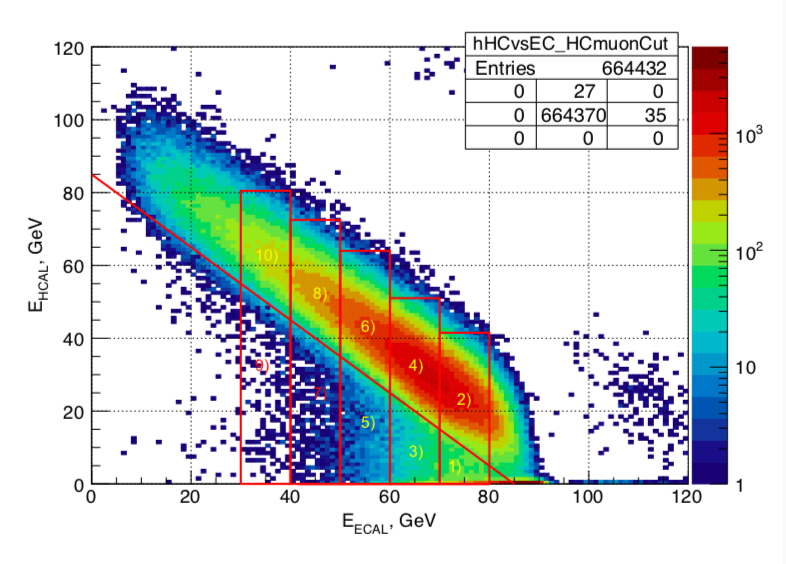
\includegraphics[width=0.45\textwidth]{\pdirthree/zones-no-veto.png}
  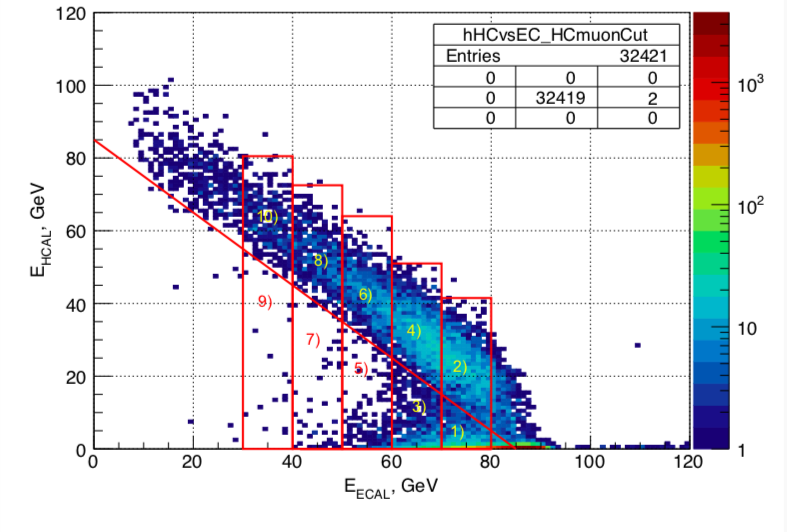
\includegraphics[width=0.45\textwidth]{\pdirthree/zones-veto.png}
  \caption[electronuclear background estimation]{Partioning of the $\ehcalplane$ into ten zones for the background estimation of electronuclear event leaking in the signal box. The left panel shows the control sample of event after clean electron are selected using SRD, tracking, pileup-removal and a hit in the central cell of the ECAL. The right panel shows the same sample after the event with signal in the VETO counter are removed. Adapted from \cite{na64-neutrals-study}.}
  \label{fig:enucl-bkg-estimation}
\end{figure}

\begin{table}[bth!]
  \centering
  \caption[Invisible mode background]{Expected background for 2.84 $\times$ $10^{11}$ EOT collected at the time this thesis was written \cite{NA64:2019imj}}
  \begin{tabular}{lr}
    \hline \hline
    Background source & Background, $n_b$ \\
    \hline
    $\pi^-$,$\mu^-$ punchthrough                      & $<10^{-14}$ \\
    low energy $e^-$                                  & $<10^{-12}$?? \\
    $e^-$/hadron nuclear interaction in target        & $<0.044$ \\
    $\pi^-$,$\mu^-$, $K_{3e}$ decay                    & 0.02 $\pm$ 0.01 \\
    $e^-$ nuclear interaction in the  beam line       & 0.43 $\pm$ 0.16 \\
    \hline
    Total (conservatively)                            & 0.53 $\pm$ 0.17 \\
    \hline \hline                       
  \end{tabular}
  \label{tab:inv-bkg}
\end{table}

\subsection{Visible mode background}

It is straight forward to understand that the background signature differs significantly in the visible mode setup. Since now the signal requires the sum of the two calorimeters (WCAL and ECAL) energy deposited to be equal to the incoming primary energy, we no longer have the problem of some particle escaping the setup in the transverse direction. Because of the large distance between the WCAL and ECAL\footnote{7.5 \si{\meter} in the 2018 setup, 4.2 \si{\meter} in the 2017 setup}, such event is actually very likely. The background in this case can be caused by particles able to punch-through the first target without leaving any energy deposit in the W2 counter placed immediately after and then leave a pure electromagnetic signature in the ECAL downstream. Because of the different length of the setup and the addition of a vacuum tube (see Fig.\ref{fig:setup-vis-2018}), the background calculated for 2017 and 2018 differs significantly. The exact suppression depends on the exact source of background considered, but it can amount up to one order of magnitude \cite{Banerjee:2019hmi}. Alternatively to the method used in \cite{Banerjee:2019hmi}, this thesis presented an alternative approach that relies on the GEM trackers to boost the signal yield. The method is detailed in Sec.\ref{ch3:sec:vis-mode-tracking}, and consist in applying a final discrimination to the event based on a tracking procedure instead of the W2 counter when the energy detected in the ECAL is smaller than 75 \gev. The background condition do not differ significantly, and are reported in Tab.\ref{tab:vis-bkg}


\subsubsection{Hadronic background}
\label{ch3:sec:bkg:vis:hadr}

Starting from the most simple scenario, punch-through of $\pi^-$ can be a background if the leave no energy in the W2 counter, an energy $> 2\emip$ in S4, and then deposit the rest of their energy in the ECAL. The product of these probabilities was conservatively estimated to be $< 10^{-12}$ when factoring SRD and HCAL suppression. Inelastic scattering in the WCAL, for example in the form of $\pi^- + p \rightarrow (\geq 1)\pi^0 + (neutrals)$ can be a source of background as they can punch-through the W2. This background was estimated using the extrapolation of the charge-exchange cross section, measured on different nuclei, after taking into account SRD rejection. In the tracking-analysis, inelastic scattering in the WCAL produces a large occupancy in the decay volume that can potentially create vertex candidates. Such events are expected to be suppressed by the selection criteria applied downstream for hadron rejection outlined in Sec.\ref{ch3:sec:selection-criteria-vis}. Furthermore, events able to mimic the pure electromagnetic signal of the decay $\DM \rightarrow e^+ e^-$ are often accompanied by a large transversal spread and are thus rejected by the requirement of energy conservation at a level of $< 10^{-5}$. This estimate was obtained by integrating the events in the signal region with two tracks in the decay volume without applying any rejection criteria for hadrons in a $\pi^-$ simulation. Such an event should also pass the independent selection criteria applied upstream, namely large energy deposited in the SRD and WCAL pre-shower. In a sample up to $10^7$ EOT, it was not possible to find an event with such signature even after removing the HCAL and VETO from the selection criteria.

To estimate the background for a larger number of EOT, the $\ks$ decay was used as a benchmark process, as its short decay length is expected to be compatible with the ones of the $\DM$. The energy spectrum of $\ks$ was simulated using an exponential distribution with an energy cut-off of 18 GeV, as $\ks$ below this energy have a negligible probability to decay outside the dump. To estimate the number of $\ks$ in the sample, neutrals event were selected by applying all selection criteria to the control sample but changing the requirement for $S4$ to $E_{S4} < 0.5 \emip$. The distribution of these events is shown in Fig.\ref{fig:w-e-vis}, here we label signal-like the events that passed all selection criteria in the control sample. One such events was recorded in 2017, well outside of the signal region. In 2018 the number of neutral was reduced by a factor 2-3, and no signal-like events was observed. These data were used to estimate the ratio between neutral and signal-like event using the MC-simulation of $\ks$. This resulted in an estimate of 0.06 events for the 2017 data and 0.005 events for 2018 data. Statistical fluctuation of the data dominates the error for this estimate.

To estimate the background for the tracking analysis, tracking-criteria were applied over the $\ks$ MC-sample. It was estimated that a rejection of $10^{-2}$ can be conservatively achieved for this background using the opening angle of the reconstructed vertex as discriminator. This estimate however mostly depends on the main hadronic decay channel $\ks \rightarrow \pi^- + \pi^+$ which is further suppressed downstream by the hadron suppression cuts such as no energy deposited in the HCAL and in the VETO. The decay channel $K^0_S \rightarrow \pi^0 + \pi^0$ has on the other hand a small chance to leave any signature in the GEM modules as no charged particle is typically emitted. Signal-like events can be produced either by the conversion of a photon from the $\pi^0 \rightarrow \gamma \gamma$ decay into a $\pair$ pair or in the decay chain $\ks \rightarrow \pi^0 + \pi^0, \pi^0 \rightarrow \gamma + e^- + e^+$. This last channel is however suppressed by its low branching ratio $\Gamma_i$/$\Gamma \approx $1\% \cite{review-particle-physics}. A dedicated simulation performed with biased branching ratio shows that the rejection for this channel is further improved to $< 10^{-3}$ since the large emission angle of a three-body decay is significantly different from the one expected in the $\xdecay$ decay. A conservative rejection of $\sim 10^{-5}$ is reached accounting both suppression factors. If we add the suppression factor coming from the angle using the trackers to what was computed for the calorimeter-analysis, one can conservatively estimate the background contribution from $\ks$ to be at a level of $<0.001$.


\begin{figure}[bth!]
  \centering
  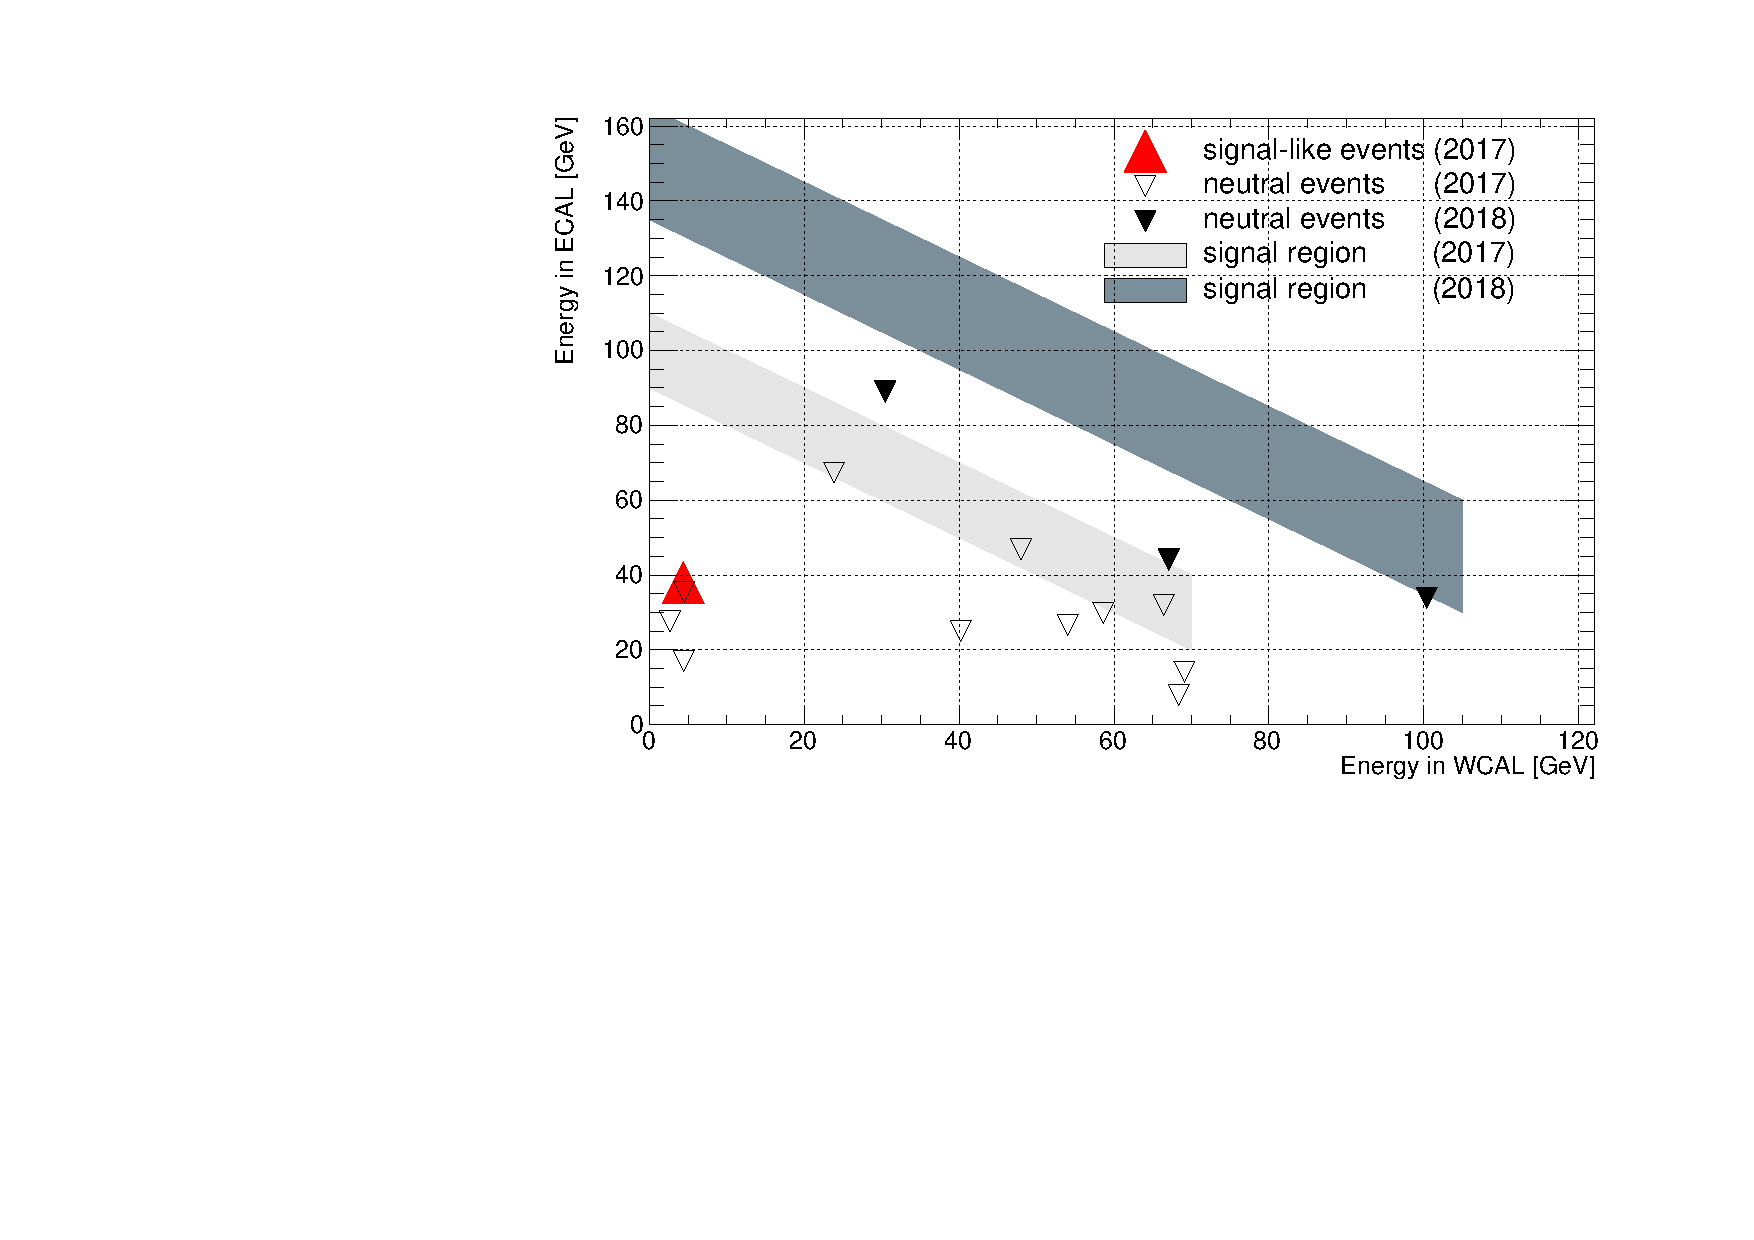
\includegraphics[width=\textwidth]{\pdirthree/w-e-neutrals.pdf}
  \caption[neutral events in visible mode]{Distribution of selected signal-like events in the $\ehcalplane$ plane for 2017 and 2018 data. Neutral events are shown as hollow (2017) and full (2018) triangles. The two shadowed bands represent the signal box region for the two different runs. A single signal-like event detected during the 2017 run not falling into the signal region is shown with a red triangle.}
  \label{fig:w-e-vis}
\end{figure}

Possible background 

\subsubsection{Muonic background}
\label{ch3:sec:bkg:vis:muon}

Background coming from $\mu^-$ primaries is very suppressed for the visible mode, and is in dominated by the probability of punch-through $\mu^-$ that leaves most of its energy inside the ECAL. This is similar to a $\pi^-$ punch-through, with the difference that the probability of it happening is lower due to both beam suppression and the absence of strong interaction for this particle. The background can be conservatively estimated to be $<10^{-14}$.

\subsubsection{Electronic background}
\label{ch3:sec:bkg:vis:elec}

The main contribution of the background from $e^-$ primary is the punch-through of high-energetic $\gamma$ that converts on the last tile of the WCAL or some material downstream and produce an $\ee$ pair. Since this background depends on large longitudinal fluctuation of the em-shower, it is hard to predicted using MC-simulations. To estimate such contribution for $\sim10^{11}$ EOTs a data-driven method is used. A sample of 3$\cdot 10^9$ EOT was considered, roughly corresponding to $\sim$10\% of the data collected in 2018. Events in the signal region with $E_{ECAL} < 105$ GeV were selected with the requirement of at least two hits in each GEM module. Only one event with such property was found. Assuming a suppression due to the angle and minimal vertex requirement of $10^{-3}$ or $S4$ selection criteria this would push our background down conservatively to a level $<10^{-3}$. The analysis of the full 2018 data is compatible with this estimate: a total of three events were found with 2 two hits in the GEM modules. For none of these events it was possible to reconstruct a physical vertex, suggesting that these particles experienced large multiple-scattering inside the WCAL before reaching the GEMs.



\begin{table}[bth!]
  \centering
  \caption[Visible mode background]{Expected background for 5.5$\times$ $10^{10}$ EOT collected in 2017 \cite{Banerjee:2018vgk} and the 3.3$\times$ $10^{10}$ EOT collected in 2018 \cite{Banerjee:2019hmi}. The third column shows background for 2018 including the GEM trackers in the analysis.}
  \begin{tabular}{lrrr}
    \hline \hline
    Background source                           & $n_b$ (2017)      &  $n_b$ (2018)   & $n_b$ (2018, new analysis)\\
    \hline
    $\pi^-$ punch-through                        & 0.0015$\pm$0.0008 &  0.0007$\pm$0.0004      \\    
    $\ks \rightarrow \pi^0 \pi^0$                     & 0.06$\pm$0.034    & 0.005$\pm$0.003 &     0.001$<$\\
    $e^-$/hadron nuclear interaction  & 0.01$\pm$0.004    & 0.01$\pm$0.004  & \\    
    $\mu^-$ punch-through                        & $<0.001$ & $<0.001$ & $<0.001$       \\            
    $\pi^-$,$K^- \rightarrow e\nu$ $K_{4e}$              & $<$0.001 & $<0.001$ & $<0.001$\\
    $eZ \rightarrow e Z \mu^+\mu^-;\mu^{\pm}\rightarrow e^{\pm}\nu\bar{\nu}$ & $<$0.001 & $<0.001$ & $<0.001$\\
    punch-through $\gamma$ & $<$0.001 & $<$0.0005 & $<$0.001 \\
    \hline
    Total (conservatively)                      & 0.07 $\pm$ 0.035   & 0.006 $\pm$ 0.003  & 0.006 $\pm$ 0.003\\
    \hline \hline                       
  \end{tabular}
  \label{tab:vis-bkg}
\end{table}



\subsection{Heavy charged particle rejection using synchrotron radiation}
\label{ch3:sec:bkg-srd}

The rejection of heavy charged particle is one of the main tool to reject the contamination of $\pi^-$,$K^-$ and $\mu^-$ present in the beam. The working principle of this method is simple in its approach. Particle traveling through a magnetic field will emitted synchrotron radiation. With minimal assumptions, the total power after a full cycle can be calculated is the useful formula :

\begin{equation}
  \label{eq:srd-power}
  P = \frac{q^2 c}{6 \pi R^2}\frac{E^4}{m^4}
\end{equation}

Here R is the bending radius experienced from the particle when inside a magnetic field B perpendicular to its velocity. From this equation, we see that the total power scales to $P\sim E^4/m^4$. This both means that the technique is suitable for high-energy particle, as the signal will be boosted, and is useful to separate particles with large differences in the mass spectrum. The difference in mass between the electron and all other particles is so large in fact that effectively no radiation is emitted at the energy of the H4 beam line. 

Simulation of the expected SR signal was performed with the Geant 4 package\cite{ALLISON2016186,1610988,AGOSTINELLI2003250}.
The geometry of the NA64 experiment was coded in Geant 4, including the 200 $\mu$m mylar vacuum windows, the detailed composition of the trackers, scintillators and the residual gas was set at a level of $10^{-3}$ mBar as in the measurements. Saturation of BGO was taken into account using Birks' law with the constants taken from \cite{AVDEICHIKOV2002251}.

The expected SR spectra for pions and electrons with energies of 50 GeV and 100 GeV are shown in Fig. \ref{fig:SRspectrum}. The plot shows the expected dependence on the incoming electron energy in the emission spectra for the realistic experimental conditions. Moreover, the comparison between the SR spectra of pions and electrons illustrates clearly the principle of this technique that allows to discriminate between them by requiring an energy threshold in the synchrotron detector.  For pions, one can see that the probability of detecting an event with energy above 1 MeV is about $\sim 10^{-3}-10^{-4}$.
These SR-like signals originate from the interactions of the incoming pions with materials placed along the beamline. Although in first approximation the energy transfer due to ionization is in the order of few \si{\kilo\electronvolt}, rare high energy transfer is also possible. The distribution of such secondary electrons with
kinetic energy $T\gg I$, where $I$ is the mean excitation energy of the
atom/molecule, for a particle with velocity $\beta=v/c$ and charge $z$
passing through a material with atomic number $Z$, mass number $A$ and
thickness $dx$ is described by \cite{review-particle-physics}:
\begin{equation}
\frac{d^2N}{dTdx} = \frac{1}{2}K z^2 \frac{Z}{A}
\frac{1}{\beta^2}\frac{F(T)}{T^2}
\label{eqn:knock-on}
\end{equation}
The constant $K$ is defined as $K=4\pi N_A r_e^2 m_e c^2$ where N$_A$ is
the Avogadro's number, $r_e$ is the classical electron radius and $m_e$
the electron mass.
$F(T)$ is a spin-dependent factor, which in our case for $T \ll W_{max}$
is very close to unity. W$_{max}$ is the maximal energy transfer in a single collision to the
electron:
\begin{equation}
W_{max} = \frac{2m_e c^2 \beta^2 \gamma^2}{1+ 2\gamma m_e/M+(m_e/M)^2}
\end{equation}
For a $\pi^-$ at 100 GeV, $W_{max}$ is roughly 1 GeV which
covers completely the energy range where synchrotron radiation is
emitted. Eq.\ref{eqn:knock-on} is valid in the range $I\ll T \leq W_{max}$.
 \par 
Furthermore, Geant 4 reproduces the critical energy $E_c$ which divides the spectrum into two parts of equal power is:
\begin{equation}
E_c = \frac{3 \hbar c \gamma^3}{2R}
\end{equation}
with the reduced Plank constant $\hbar$ and the bending radius $R$. 
 For 100 GeV electrons in the  $B=1.7$ T bending field this corresponds to $E_c\sim$11.35 MeV. The expected mean energy of a synchrotron photon $E_m=E_c/\pi\simeq 3.6$ MeV is in very good agreement with simulation. The number of photons emitted per revolution in this energy range in the field of 7 T$\cdot$m is defined as:
\begin{equation}
N_\gamma = \frac{5 \pi \alpha}{\sqrt{3}}\gamma
\end{equation}
where $\alpha$ is the fine structure constant. 
By scaling this equation for the fraction of the circle where the particles are inside the magnetic field, one obtains a mean number of emitted photon of about 24.
The SRD geometrical acceptance is about one third,  thus one can estimate that the sum of deposited energy is approximately 29.35 MeV in good agreement with the results of the simulation as shown in Fig. \ref{fig:SRspectrum}. 
 
\begin{figure}[htb!]
\centering
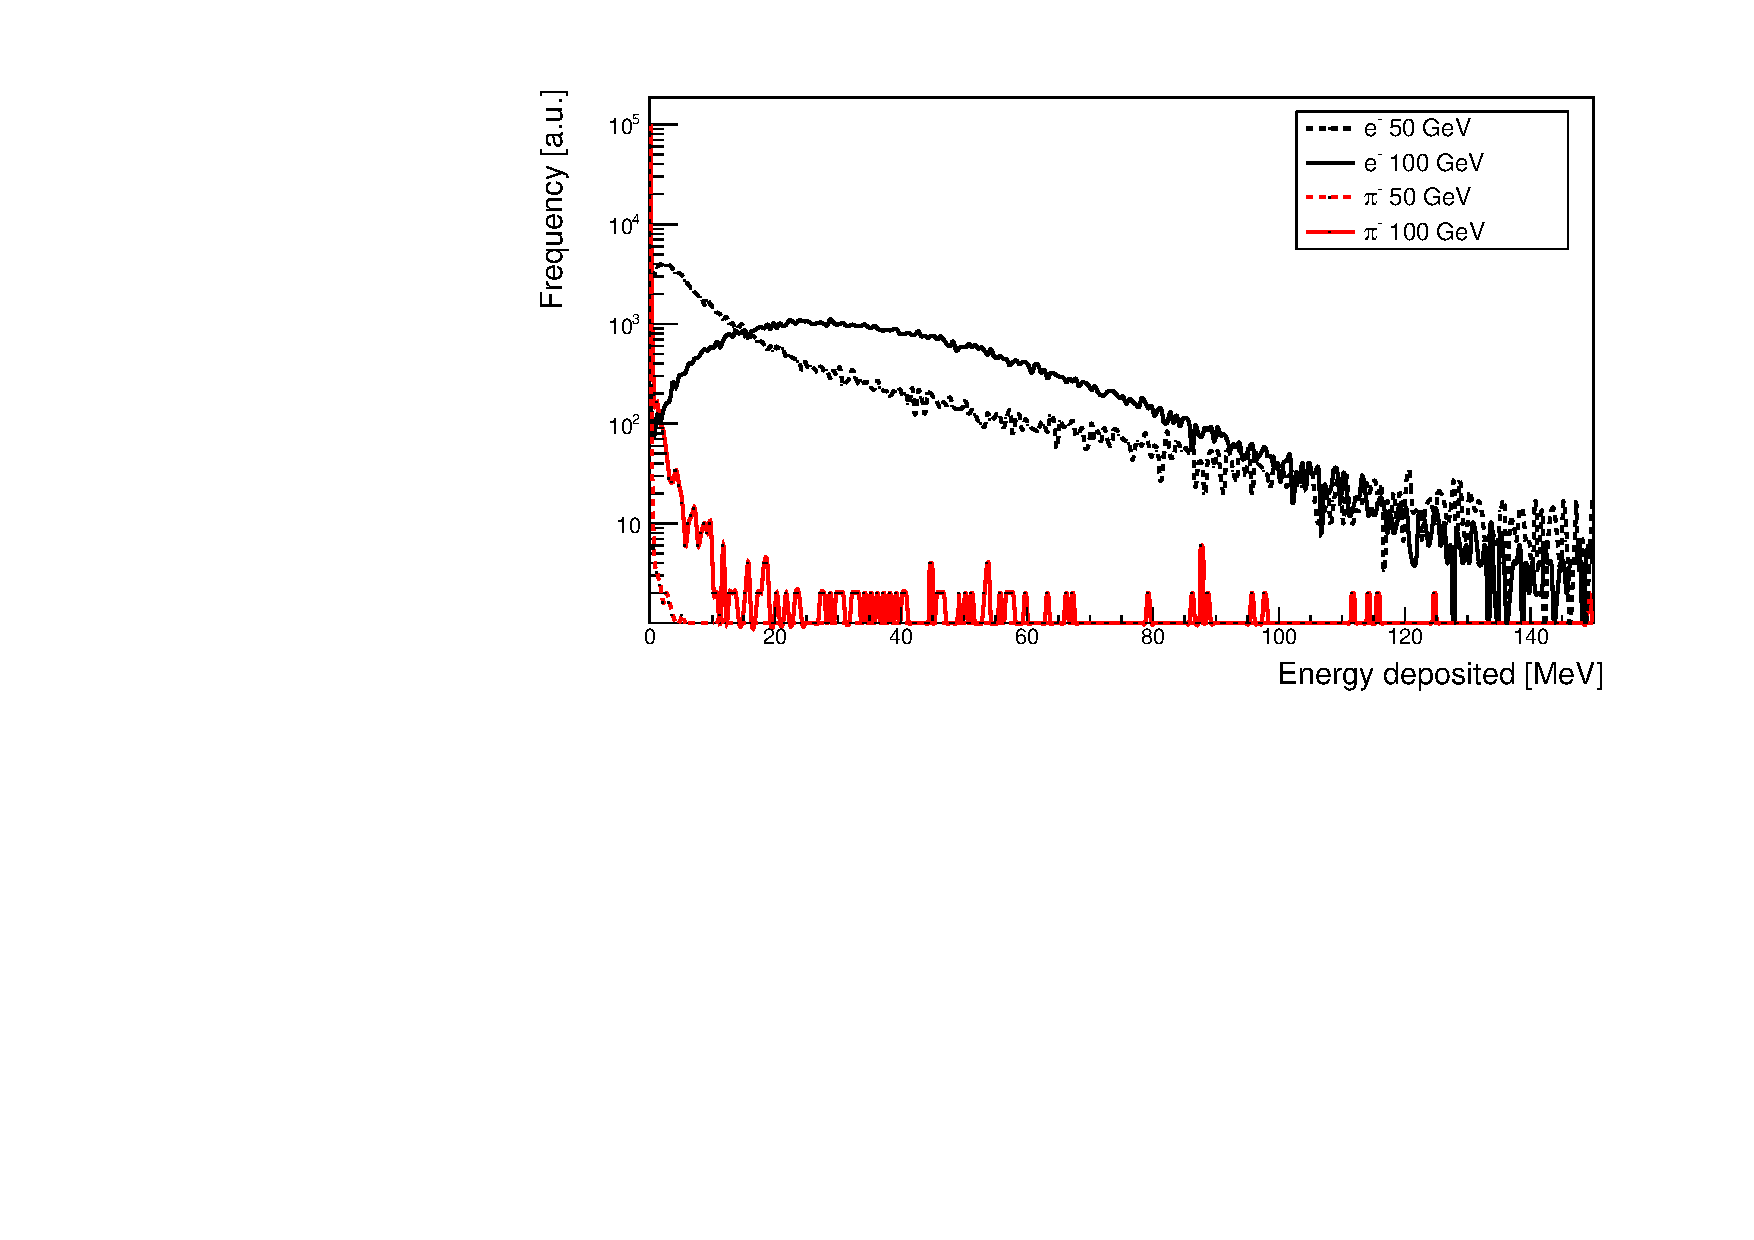
\includegraphics[width=1.\textwidth]{\pdirthree/comp_spectra.pdf}
\caption[SR spectrum for different energy detected in the SRD]{Result of the Geant 4 simulation for the energy detected by the SR detector for 50/100 GeV e$^-$(black dashed/solid line) and 50/100 GeV $\pi^-$ (red dashed/solid line).}
\label{fig:SRspectrum}
\end{figure}

The SRD detector was tested during the NA64 test beam run in July 2016. The two BGO rows are parallel to the primary beam direction as shown in Fig.\ref{fig:newgeo}. The dipole magnets installed in series produce a total integrated magnetic field of 7 T$\cdot$m \cite{Banerjee:2016tad} resulting in a nominal displacement for the incoming electrons at the SRD/ECAL positions of 31/34 cm from the undeflected beam axis. The SRD was placed between the undeflected and the deflected beam axis at a distance of approximately 9 cm from both (Fig.\ref{fig:newgeo}). This separation minimises the possibility for Bremsstrahlung photons and neutral particles produced by interactions of the beam particle with materials upstream and for particles in the beam halo to hit the SRD. In fact, such interactions result in the saturation of the SRD with a significant loss of efficiency due to the long decay time of the BGOs.

%The expected Landau distribution of energy deposits was fit to the data to find the mean peak position to extract the calibration constant. 

The two crystals facing the beam (labeled 3 and 7 in Fig. \ref{fig:newgeo}) detect most of the energy emitted by synchrotron radiation. We will refer to those as SRD BGOs from now on. The remaining six crystals are used to detect events with high energy deposition in the SRD. In particular the last two crystals of each row (labeled 0 and 4 in Fig. \ref{fig:newgeo}) detect some energy only in the case of very energetic Bremsstrahlung events and thus can be used as a veto (see Fig.\ref{fig:newgeo}). The six crystals after the SRD BGOs act also as a shield from backscattering particles coming from the ECAL suppressing pions by an additional order of magnitude. Finally in this geometry it is possible to use the coincidence of the two SRD BGO crystals to improve the tagging of synchrotron photons by rejecting knock-on electrons produced by incoming pions. In fact synchrotron radiation has a homogenous spectrum in the whole arc described by the primary and deflected beam and thus a signal is detected in both SRD BGOs. On the contrary, electrons generated by a $\pi^-$ undergoing ionisation will mostly leave energy only in a single crystal as illustrated in Fig. \ref{fig:newgeo}. 
With the requirement of detecting in both SRD BGOs an energy deposition above a 1 MeV the suppression factor is improved up to a level of $10^{-5}$.



\begin{figure}[htb!]
  \centering
  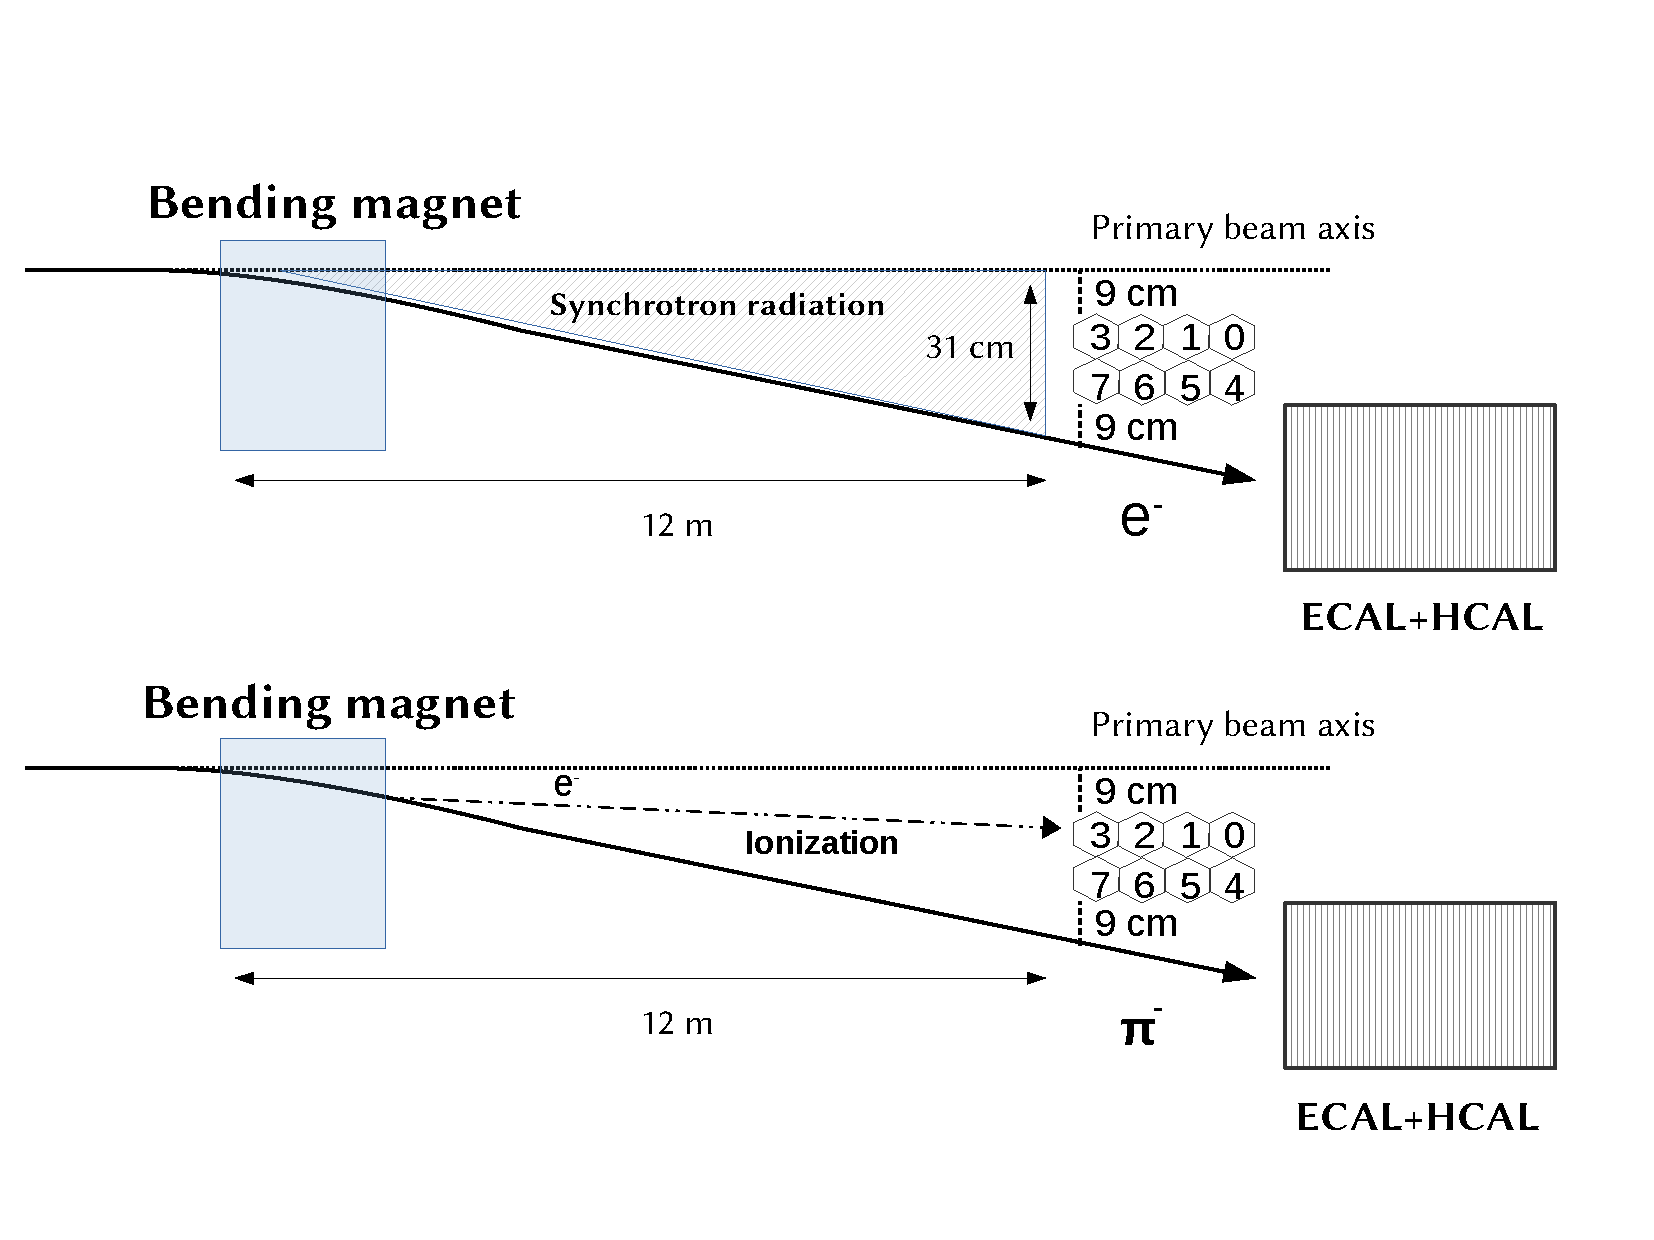
\includegraphics[width=.9\textwidth]{\pdirthree/sketch.pdf}
  \caption[Geometry of the BGO crystals]{Geometry of the BGO crystals. Crystals 7,3 (SRD BGO) collect most of the synchrotron radiation spectrum. Crystals 4,0 (VETO BGO) on the other hand are effected only in case of a high energy event and are thus used as a veto. The remaining crystals serve as a shield for the SRD from backscattering particles coming from the ECAL. Top: illustration of event leaving a SR signal in the SRD. Bottom: illustration of a SR- like signal in the SRD for a knock-on electron produced by pions.}
\label{fig:newgeo}
\end{figure}

Data with a 100 GeV $\pi^-$ beam were taken to have a direct measurement of the suppression factor achievable through synchrotron radiation measurements. The beam intensity was 5.3$\times 10^4$ particles per spill. The trigger was given by the coincidence of the three plastic scintillator counters (S1, S2 and S3 shown in Fig.\ref{fig:setup-invis-2018}). The additional requirement of an energy deposition below 60 GeV in the ECAL was applied in order to completely reject electrons from the $\pi^-$ sample of $\sim 10^5$ collected events.

For the 100 GeV electron beam run, a total of 220 spills were recorded with an intensity of 3.4$\times 10^5$/spill. 
The same trigger used in the pion run was used for the electron data.
In this case though, in order to reduce the pion contamination which is at a level of few \% and obtain a pure sample of electrons-only events with a total energy deposition in ECAL + HCAL above 90 GeV but with less than 20 GeV energy in the HCAL were used.  


The energy spectra recorded by the SRD BGO with electrons and pions are shown in Fig.\ref{fig:comp_spectra}. The SR spectra obtained with the electron beam are used to perform the BGO calibration by comparison with the simulation. With this method a very good agreement of data and MC is achieved (see plot on the left of Fig.\ref{fig:comp_spectra}). As a cross check, using the obtained calibration constants, the data from the pion beam impinging directly on the SRD are fitted with a Landau distribution. The obtained peak position of 60 MeV is in good agreement with the prediction of the MC. 

Time coincidence of signals above the energy threshold of 1 MeV from both SRD counters is required and high energy Bremsstrahlung events are removed using the veto BGO.
The suppression of synchrotron radiation emission detected for pions compared to electrons is clearly visible by comparing the two plots. For the electron spectrum, a 1\% pileup beam events have been added to the simulation as predicted for the given spill intensity and with the known decay time of BGOs.  Both spectra are in very good agreement with the simulation.

\begin{figure}[htb!]
  \centering
  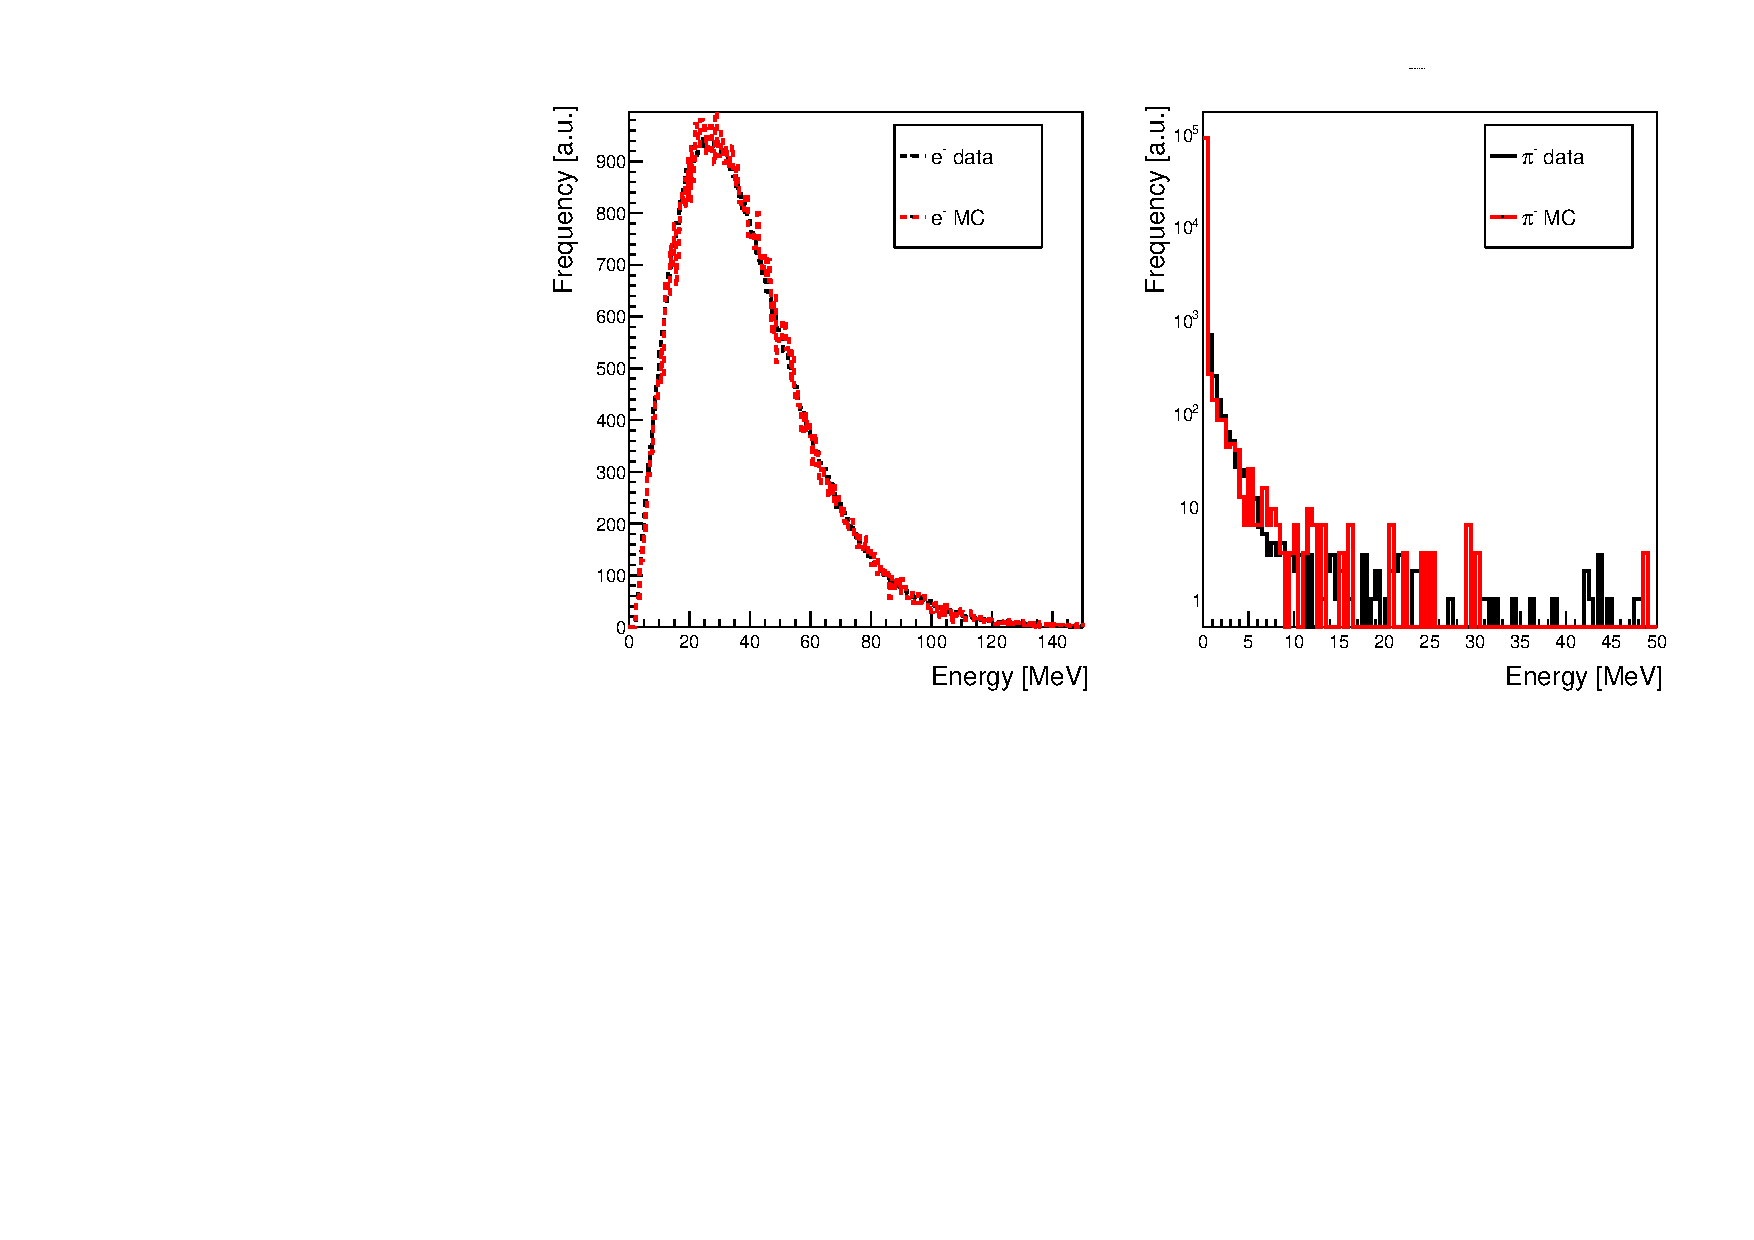
\includegraphics[width=1.\textwidth]{\pdirthree/spectra_tot.pdf}
  \caption[SRD comparison between data and MC]{Comparison between data and simulation (MC) of the synchrotron radiation spectrum detected for 100 GeV electrons (left) and pions (right). }
  \label{fig:comp_spectra}
\end{figure} 

\begin{figure}[htb!]
  \centering
  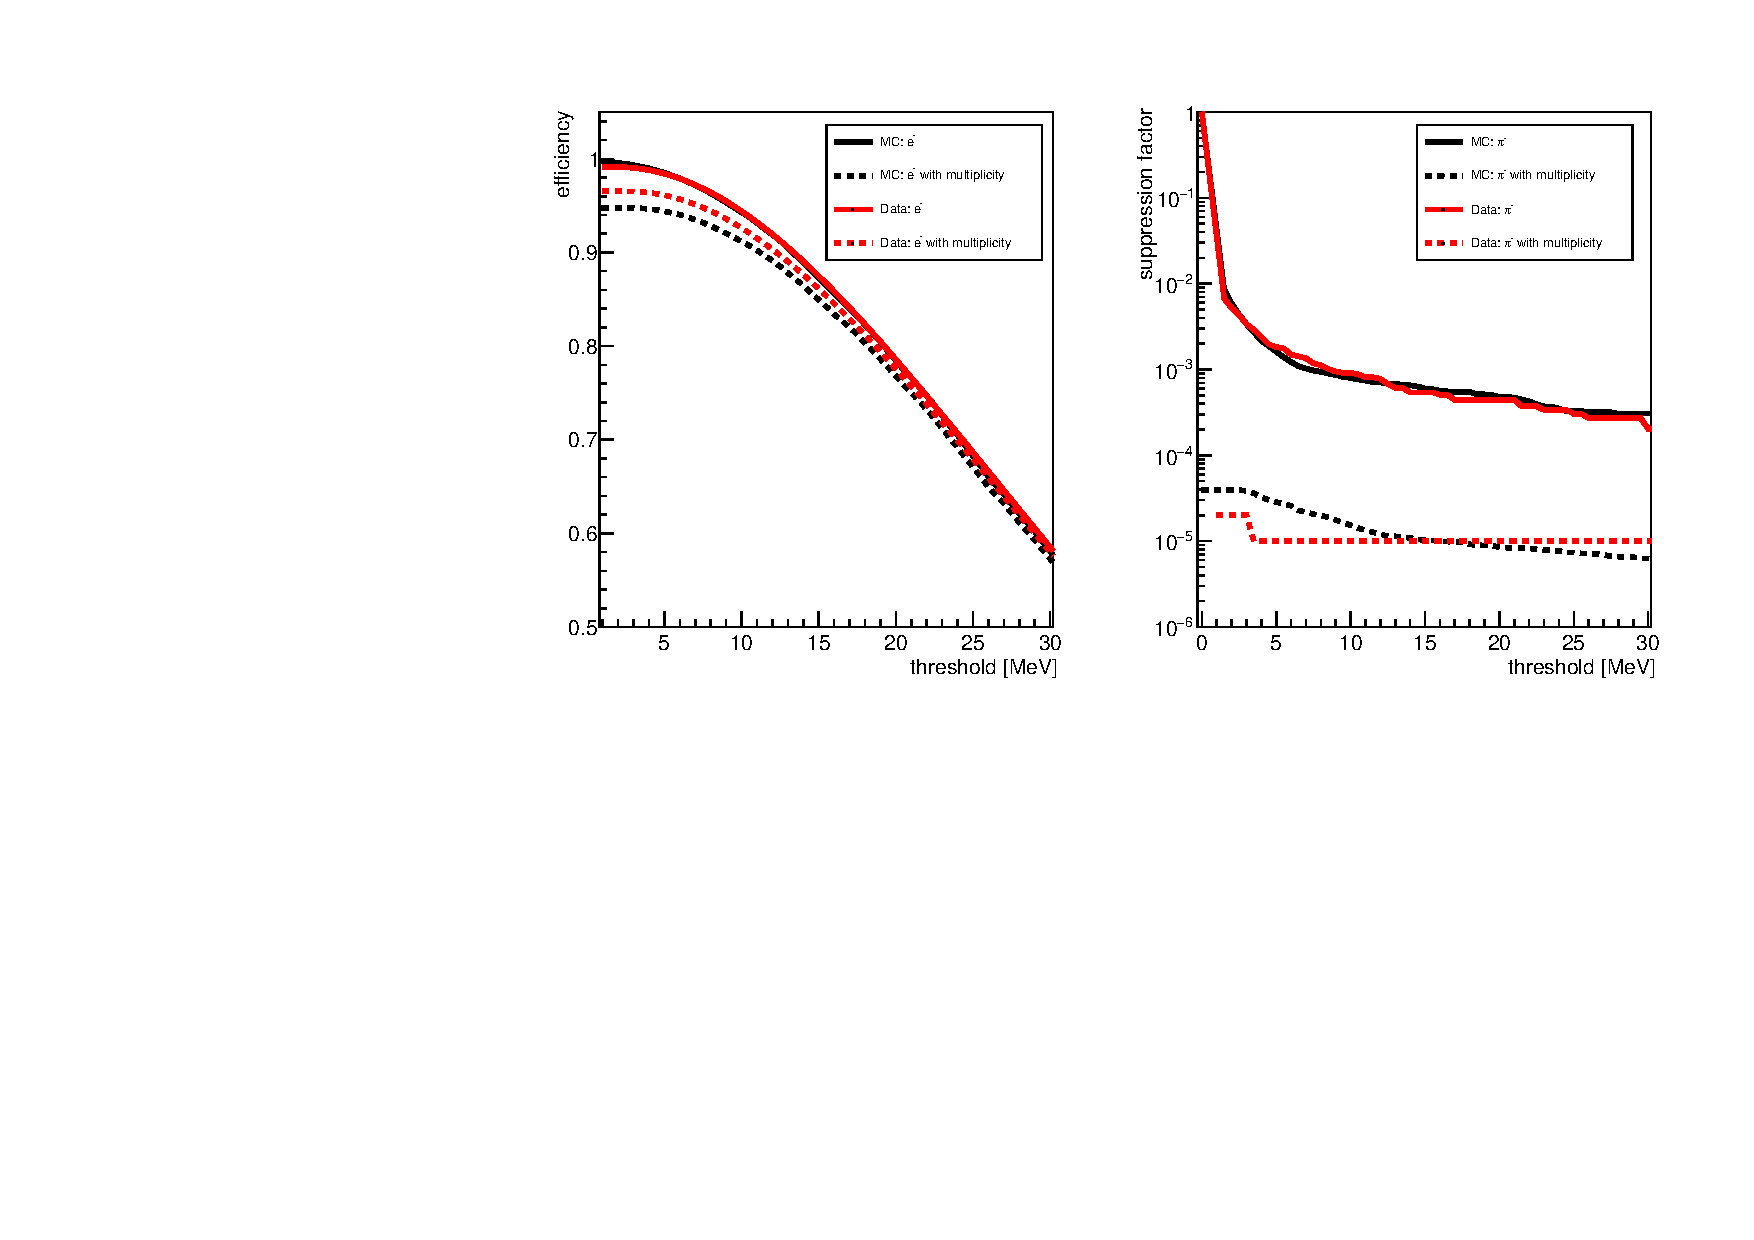
\includegraphics[width=1.\textwidth]{\pdirthree/sup_mult.pdf}
  \caption[efficiency and rejection power of the SRD cut]{Left: Comparison between data and simulation (MC) for electrons of the efficiency as a function of threshold set on the total energy deposited in the SRD BGO and for the requirement that this is deposited in each single crystal (multiplicity). Right: Comparison between data and simulation for pions and electrons of the suppression factor as a function of the threshold set on the total energy deposited in the SRD BGO and for the multiplicity requirement.}
  \label{fig:sup_mult}
\end{figure}

The efficiency for the electrons and the suppression factor for the pions are plotted in Fig. \ref{fig:sup_mult} as a function of the threshold on the energy deposited in the SRD. We distinguish between two cases:
\begin{enumerate}
\item The threshold is set on the total energy deposited in the SRD.
\item Both SRD signals have to be in-time and above the threshold of 1 MeV (multiplicity requirement).
\end{enumerate}
One can see that applying the criterion 2) the efficiency only decreases slightly compared to 1), while the suppression factor for pions is dramatically increased (by two orders of magnitude) with the requirement of having the two BGOs in coincidence.
This can be understood because the SR-like signal generated from secondary electron will leave a signal only in one of the two BGOs while the SR from electrons is spread out uniformly as explained above. 
This is also underlined by Tab. \ref{tab:hits} where the fraction of events with different hit multiplicity in the SRD BGO for both pion and electron runs are reported.

\begin{table}[hbt!]
\begin{center}
\begin{tabular}{cccc}
Events hit multiplicity  (\%) & 0 BGO  & 1 BGO & 2 BGOs\\
\hline
Pions & $98.77$ & $1.21$ & $1.4\times10^{-3}$  \\
Electrons & $2.4\times10^{-1}$  & $2.60$ & $97.37$ \\
\end{tabular}
\end{center}
\caption[Fraction of pion and electron events for different hit multiplicity in the SRD from the data]{Fraction of pion and electron events for different hit multiplicity in the SRD from the data.}
\label{tab:hits}

\end{table}

\subsection{Hadron rejection using electromagnetic shower profile}
\label{ch3:sec:bkg-ecal-profile}

On the top of rejection using SRD, the transversal segmentation of the ECAL offers another tools for hadron rejection. The idea is to discriminate between a classical em-shower profile to a more complex hadronic shower using a $\chi^2$-test. A shower profile database can be built by correlating the hit position (x,y) on the ECAL with the fraction of energy deposited in each ECAL cell. From this database a predicted value of energy deposited in each ECAL cell can be extracted and compared to the one of the single event. The compatibility between the predicted profile and the measured one can be tested using the $\chi^2$-distribution:

\begin{equation}
  \chi^2 = \sum^{9,36}_i \left(\frac{E_{pred}^i(x_{hit},y_{hit})-E_{mes}^i}{\sigma^{i}_{pred}(x_{hit},y_{hit})}\right)^2
  \label{eqn:chi}
\end{equation}


\begin{description}
\item[$E_{pred}^i$]: is the energy predicted by the profile of cell
  $i$
\item[$E_{mes}^i$]: is the energy measured in the cell $i$
\item[$x_{hit},y_{hit}$]: coordinates of the hit position of the
  particle in the ECAL plane
\item [$\sigma^{i}_{pred}$]: error estimated for the predicted energy
  in cell $i$
\end{description}


Two different summation indexes are used for the two different cases
where only the cells surrounding the central one hit by the beam are
used for the test (total of 9 cells) and the case where all the cells
are used (total of 36, see Fig.\ref{fig:ecal_example}).

\begin{figure}[h!]
  \begin{center}
    \includegraphics[scale=0.47,page=4]{\pdirthree/ecal_example.pdf}
  \end{center}
  \caption[ECAL sketch]{sketch of the 36 cells of the ECAL. The central cell 3X3
    were the beam is directed is plotted in red, while the cells
    surrounding it are plotted in green. On the bottom-right an
    example of how a profile for a cell looks like in the MC.}
  \label{fig:ecal_example}
\end{figure}


 
\subsubsection{Construction of the profiles}
\label{ch3:sec:make_profile}

A shower profile database can be understood as an $N\times N$ matrix
where each entry represents a portion of the ECAL cell of dimension
$d_x \times d_y$. Each entry of the matrix contains the mean value of
energy deposited in the cell when the incoming particle hits the
portion of the ECAL plane described by that entry. In order to also
account for the deviation that such shower can have as function of the
hitting point one would need a second matrix to encode such
information. To build such database the root class TProfile2D was used \cite{root-tprofile}.

The main parameters that play a role in the construction of the shower
profiles are the dimensions of the area that is covered by the
TProfile2D, and the dimensions $d_x \times d_y$ that each bin has,
which represents the minimal distance between two hit points that can
be resolved by the database.  The total dimension that the profile
should have can be trivially set to be equal to the ones of one ECAL
cell (38.2$\times$38.2 mm, see \cite{na64-detectors}) since our cuts
already requires the majority of the shower to be contained in the
cell aligned with the beam spot. The problem of the bin dimension is
more subtle: due to the shower symmetry there is no particular reason
to set $d_x \neq d_y$ the precise dimensions of the bin must be a
compromise between having a large bin that allows good statistic and a
small bin that allows enough precision. The large sample of electrons
collected in NA64 typically allows good statistic for each bin even
when their dimension is below 1 mm. However, defining a bin smaller
than the accuracy that we are able to achieve in the extrapolation of
the MicroMegas line to the ECAL should be avoided. This error can be
derived analytically to be:
\begin{equation}
  \sigma_{ECALxy} = \sigma_{mm}\sqrt{1+2t^2}
  \label{eqn:MMerror}
\end{equation}

\begin{equation}
  t = \frac{Z_{ECAL}-Z_{MM4}}{Z_{MM4}-Z_{MM3}}
  \label{eqn:T}
\end{equation}

where:
\begin{description}
\item[$\sigma_{ECALxy}$]: is the error of the hit position
  extrapolated to the ECAL in the xy-plane.
\item[$\sigma_{mm}$]: is the resolution of the hit position in each
  MicroMegas.
\item[$Z_{MM}$]: is the position in the Z-axis of the MicroMegas.
\item[$Z_{ECAL}$]: is the position in the Z-axis of the ECAL plane.
\end{description}


This results in a resolution of $\sim$130 $\mu$m for our setup. A more
complicate expression was considered to take into account possible
misinformation in the exact position of the detectors. While the exact
entrance angle of the particle was checked to have small effects on
$\sigma_{ECALxy}$, assuming some error on the exact position of the
detectors increases the error by a factor 2-4 for values around 1-2
cm. The work presented here was performed using a TProfile2D
with bin size of 0.34 mm which accounts for such uncertainties.

Electron calibration runs were used to produce the profiles in order to have a sample of electrons, cuts were applied to reject the contamination caused by the hadrons in the beam and out-of-time energy events. \\
The following criteria were applied for the profiles tested in this
note:

\begin{itemize}
\item Single cluster in each MicroMegas
\item Energy larger than 1 MeV and smaller than 70 MeV in each SRD
  plane
\item Coincidence of $\sim$1 ns between timing in cell (3,3) of ECAL
  and $S_0$ time.
\item Pedestal fluctuation less than 10 ADC in cell (3,3) and each of
  the surrounding cells.
\end{itemize}

The production of the database is done for the events
selected by computing the hit point of the incoming particle in cell
3x3 and updating the value of the corresponding bin in each of the 36
TProfile2D representing each cell. The specific value filled is the
percentage of energy deposited in the cell, i.e. $100 \times E^i/E^{tot}$.

After the profile are constructed, they can be used to calculated the compatibility of a single event with an em-shower. The algorithm for the $\chi^2$ computation works as follows:
\begin{enumerate}
\item The values of the xy coordinates of the hitting point of the
  particle are computed by extrapolating to the ECAL position the line
  passing through the hit point of the last two MicroMegas planes.
\item The predicted values $E_{pred}^i$,$\sigma^{i}_{pred}$ are read from the database in the corresponding bin
\item The values $E_{mes}^i$ are computed normalizing the energy $E^i$ of each cell to the total energy measured in the ECAL.
\item The value of $\chi^2$ is calculated using Eq.\ref{eqn:chi} and is normalized to the number of cells considered.
\end{enumerate}

\subsubsection{Results}
\label{ch3:sec:chi2-result}

To test the rejection power and the efficiency of the
method the algorithm described above was used for 3 type of samples\footnote{The database was generated using the electron  calibration runs 2363, 2182, 2410, 2406, 2438. A complete description of such runs can be found in \cite{na64-runs}. }:
\begin{itemize}
\item $\simeq$1.2$\times 10^{6}$ events acquired with an electron calibration run\footnote{run 2363}.
\item $\simeq$5$\times 10^{5}$ events acquired with an hadron calibration run\footnote{run 2204}.
\item $\simeq$8$\times 10^{5}$ events acquired using physical trigger at maximum H4 beam intensity.\footnote{run 2241, corresponding EOT before trigger suppression $\simeq 4 \times 10^{8}$}
\end{itemize}

The comparison of the normalized $\chi^2$-distribution between
electron calibration run and hadron run using information from all 36
cells is shown in Fig.\ref{fig:chi2}. Note that electrons reproduce
the expected shape of a $\chi^2$-distribution while for hadrons we
observe a displaced one incompatible with the one produced by
electrons.  The rejection and efficiency of a cut
$\chi^2 < \chi^2_{cut}$ are shown in detail in Fig.\ref{fig:eff}. For
a benchmark $\chi^2$-cut of 2 the efficiency calculated in run 2363
was $\sim 0.94$ with a rejection factor of $1.2\times 10^{-3}$
extracted from the hadron run 2204. These values as well as the ones
presented in Fig.\ref{fig:eff} are computed by looking at the total
number of events passing the cut and do not account for the impurities
in the beam.

Using information coming only from the 9 central
cells (Fig.\ref{fig:ecal_example}) appears to shift the distribution
to the left and reduce its spread ( Fig.\ref{fig:chi}) due to the
smaller number of degrees of freedom, the two methods have overall
comparable efficiency as can be seen in Fig.\ref{fig:eff} but smaller
rejection power when a typical cut is applied.  For the considered
benchmark cut of $\chi^2_{cut}=$2, the efficiency measured using only
central cells was of $\sim 0.93$\ and a rejection factor of
$3.1\times 10^{-3}$.


\begin{figure}[h!]
  \begin{center}
    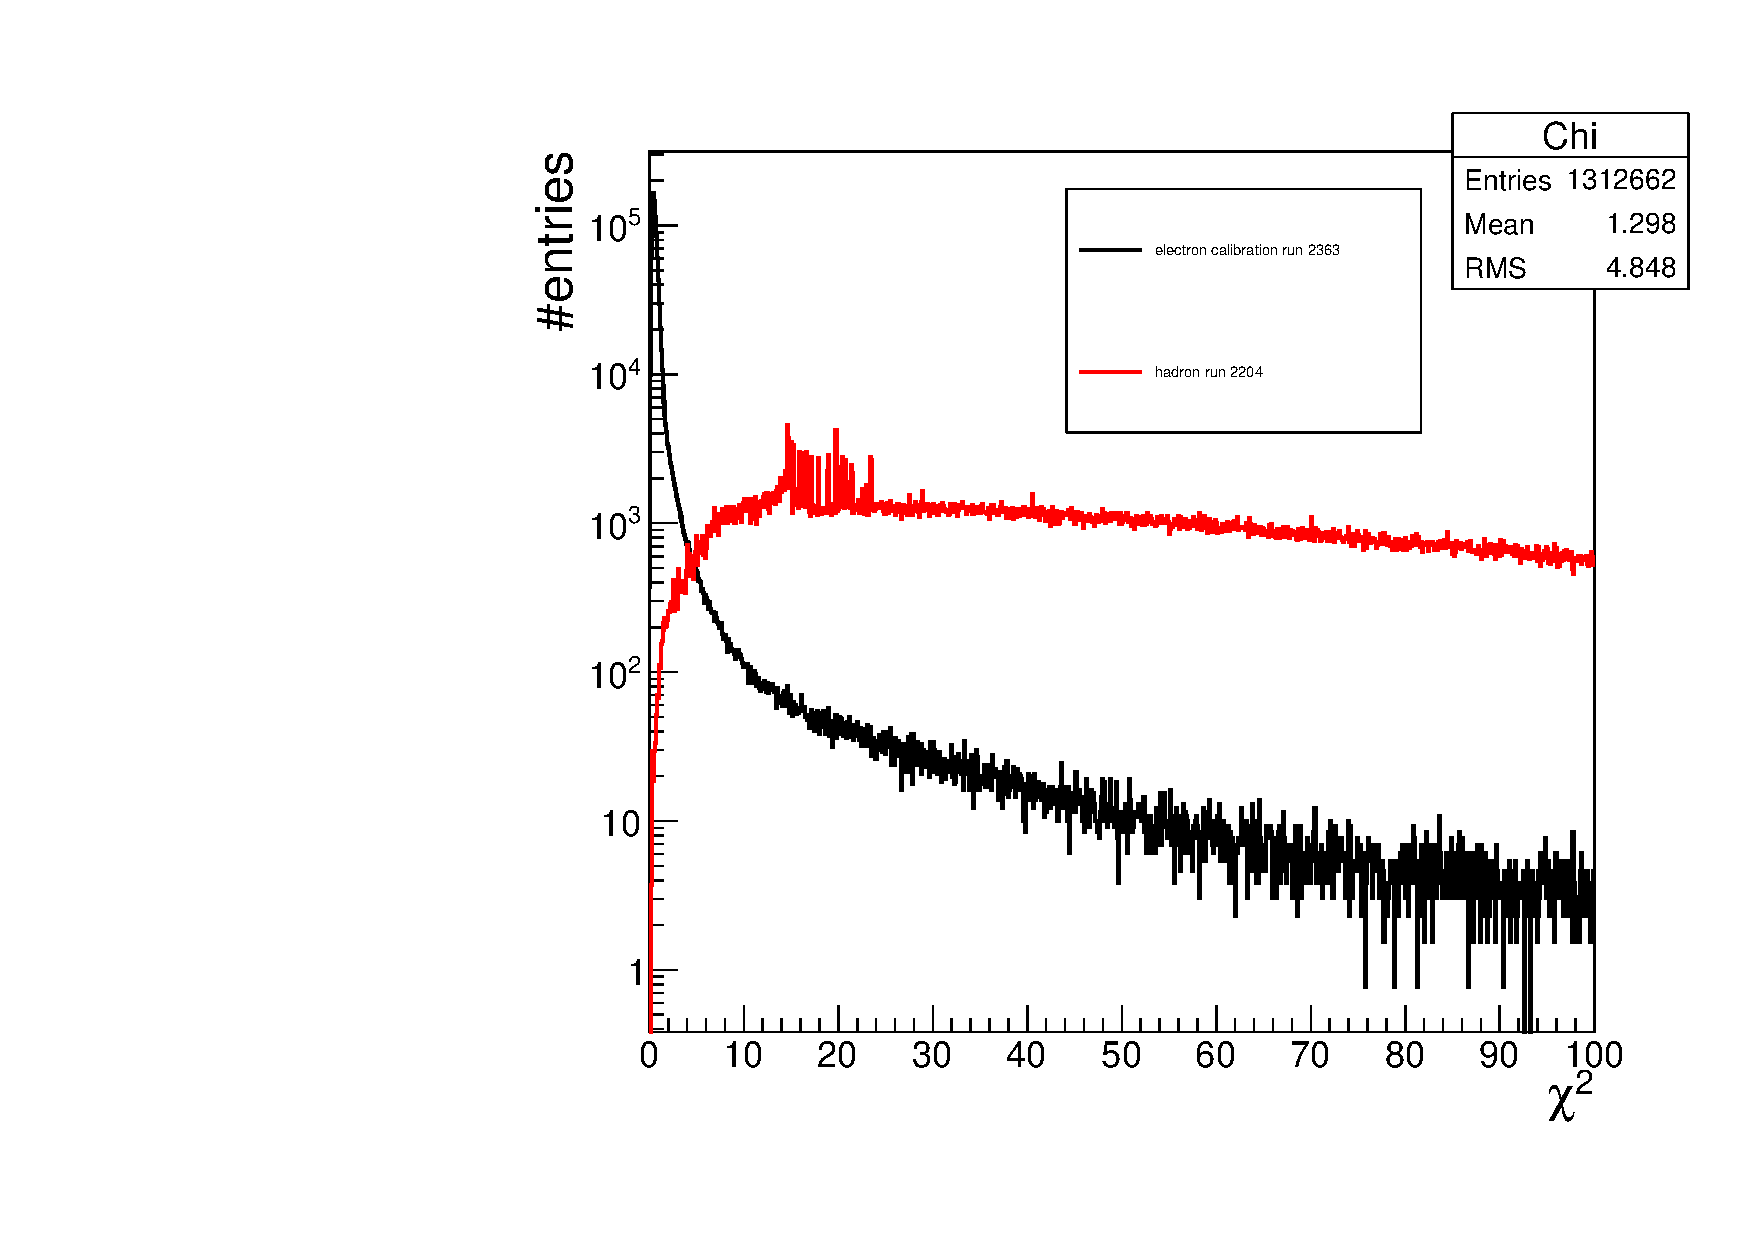
\includegraphics[width=0.95\textwidth,height=0.8\textwidth]{\pdirthree/chi_comp.pdf}
  \end{center}
  \caption[comparison between $\chi^2$ distribution, electron and hadron calibration run]{comparison between $\chi^2$ distribution generated from an electron calibration run (black) and hadron calibration run (red).}
  \label{fig:chi2}
\end{figure}

\begin{figure}[h!]
  \begin{center}
    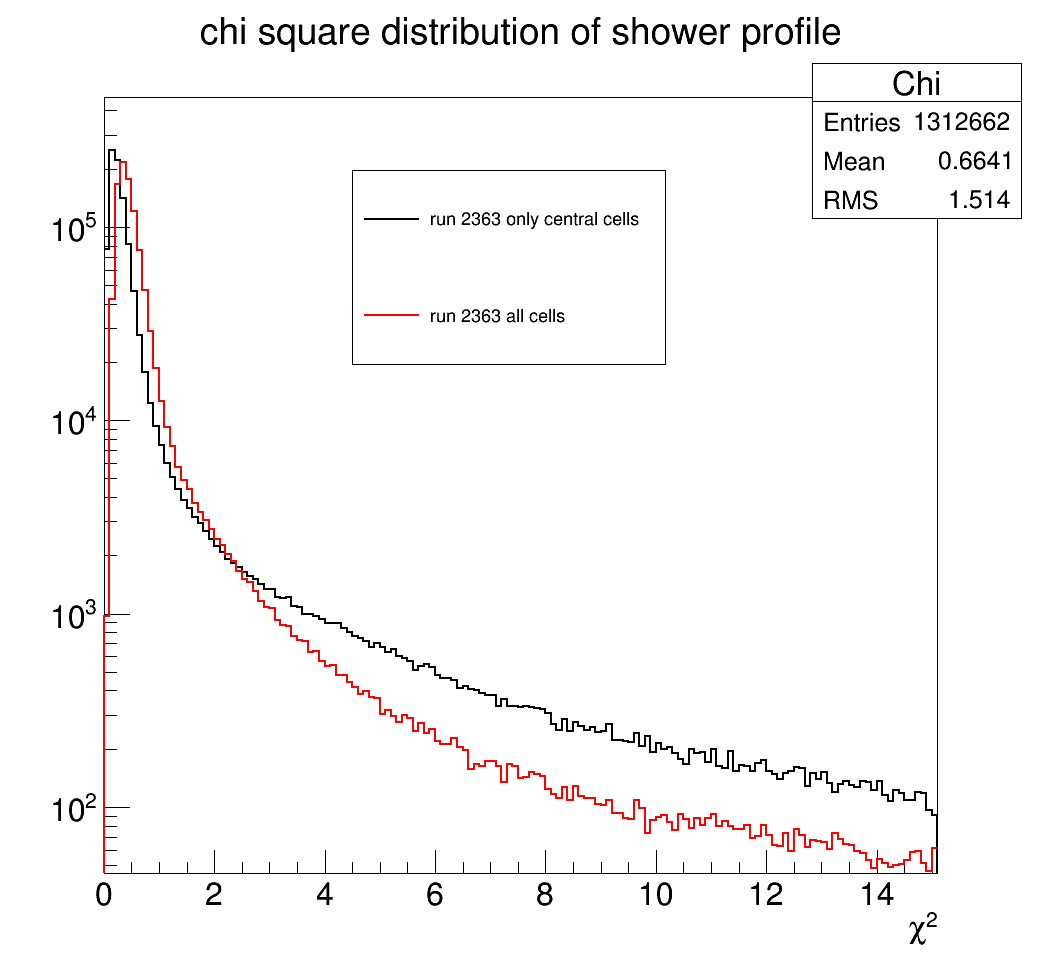
\includegraphics[width=0.95\textwidth,height=0.8\textwidth]{\pdirthree/plot_comp_cells.png}
  \end{center}
  \caption[comparison between $\chi^2$ distribution for different ECAL configurations]{comparison between $\chi^2$ distribution generated from an electron calibration run considering only central cells (black) and considering all 36 cells (red).}
  \label{fig:chi}
\end{figure}

\begin{figure}[h!]
  \begin{center}
    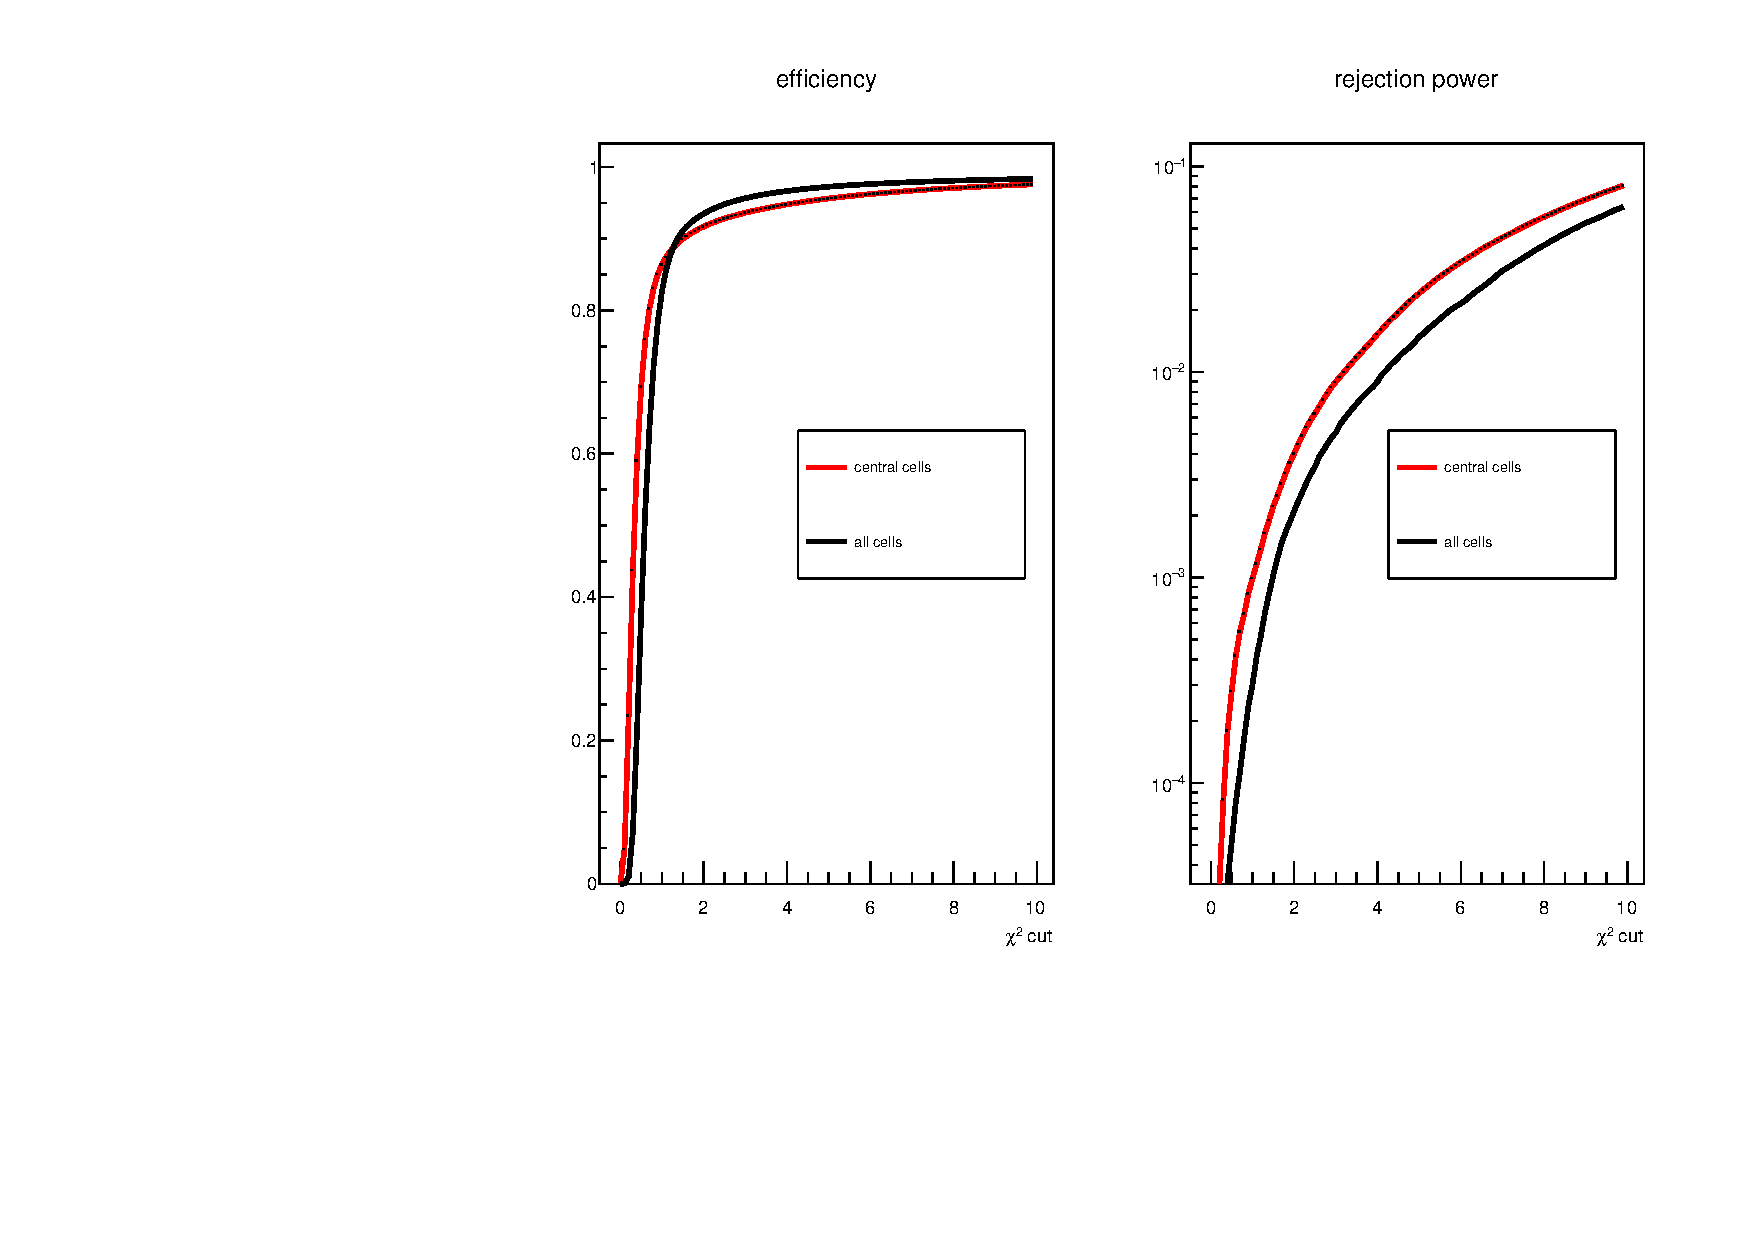
\includegraphics[width=0.95\textwidth,height=0.6\textwidth]{\pdirthree/eff.pdf}
  \end{center}
  \caption[fraction of events passing the $\chi^2$ cut]{fraction of events passing the cut $\chi^2 < \chi^2_{cut}$
    for the electron calibration run (left) and for the hadron calibration run (right).}
  \label{fig:eff}
\end{figure}

\clearpage

Different ECAL vs HCAL plots were produced to study the effect of a
$\chi^2$-cut for the run mentioned above. The one produced with
benchmark cut of $\chi^2 < 2$ are shown in
Fig.\ref{fig:ehcal_test}. The cut is shown to clean the plot in the
way expected from the hadronic activity in all selected runs. It can also
can be seen from the run recorded with physical trigger that events involving the dimuon
production $e^- \to \mu^+\mu^-$ survive the cut for energies larger
than 20 GeV.  This is expected since these events will still involve
an electromagnetic shower truncated in the moment the transition
happens. Since a possible signal from a Dark Photon would behave
similarly this suggest that the cut won't reject the signal provided
that the shower has enough energy. A similar study performed with the
MC (see Sec.\ref{ch3:sec:mc}) reached the same conclusion, however for
very small energies the shower shape will slowly reach the energy
resolution in each cell and the efficiency of the cut will drop
substantially.  The efficiency for low energy improves if only central
cells are selected for the $\chi^2$ calculation since this will reduce
the fluctuation of the single cells not involved in the shower. This
effect is shown in Fig.\ref{fig:ehcal_comp} for a cut of 2 on $\chi^2$.
\\
\\
For low energy particles it is clear that all the shower will be
contained in the cell 3x3. Below this threshold shower analysis can no
longer resolve the type of shower of the event and instead the simple
requirement of the full energy of the event to be detected by the
central cell (3x3) should be used to avoid killing the
signal. Applying a $\chi^2$-cut to a dark photon simulation (see
Sec.\ref{ch3:sec:mc}) suggested that this limit is roughly 5 GeV.  The
left plot in Fig.\ref{fig:ehcal_comp} is compatible with this
estimate.


\newpage
\begin{figure}[h!]
  \begin{center}
    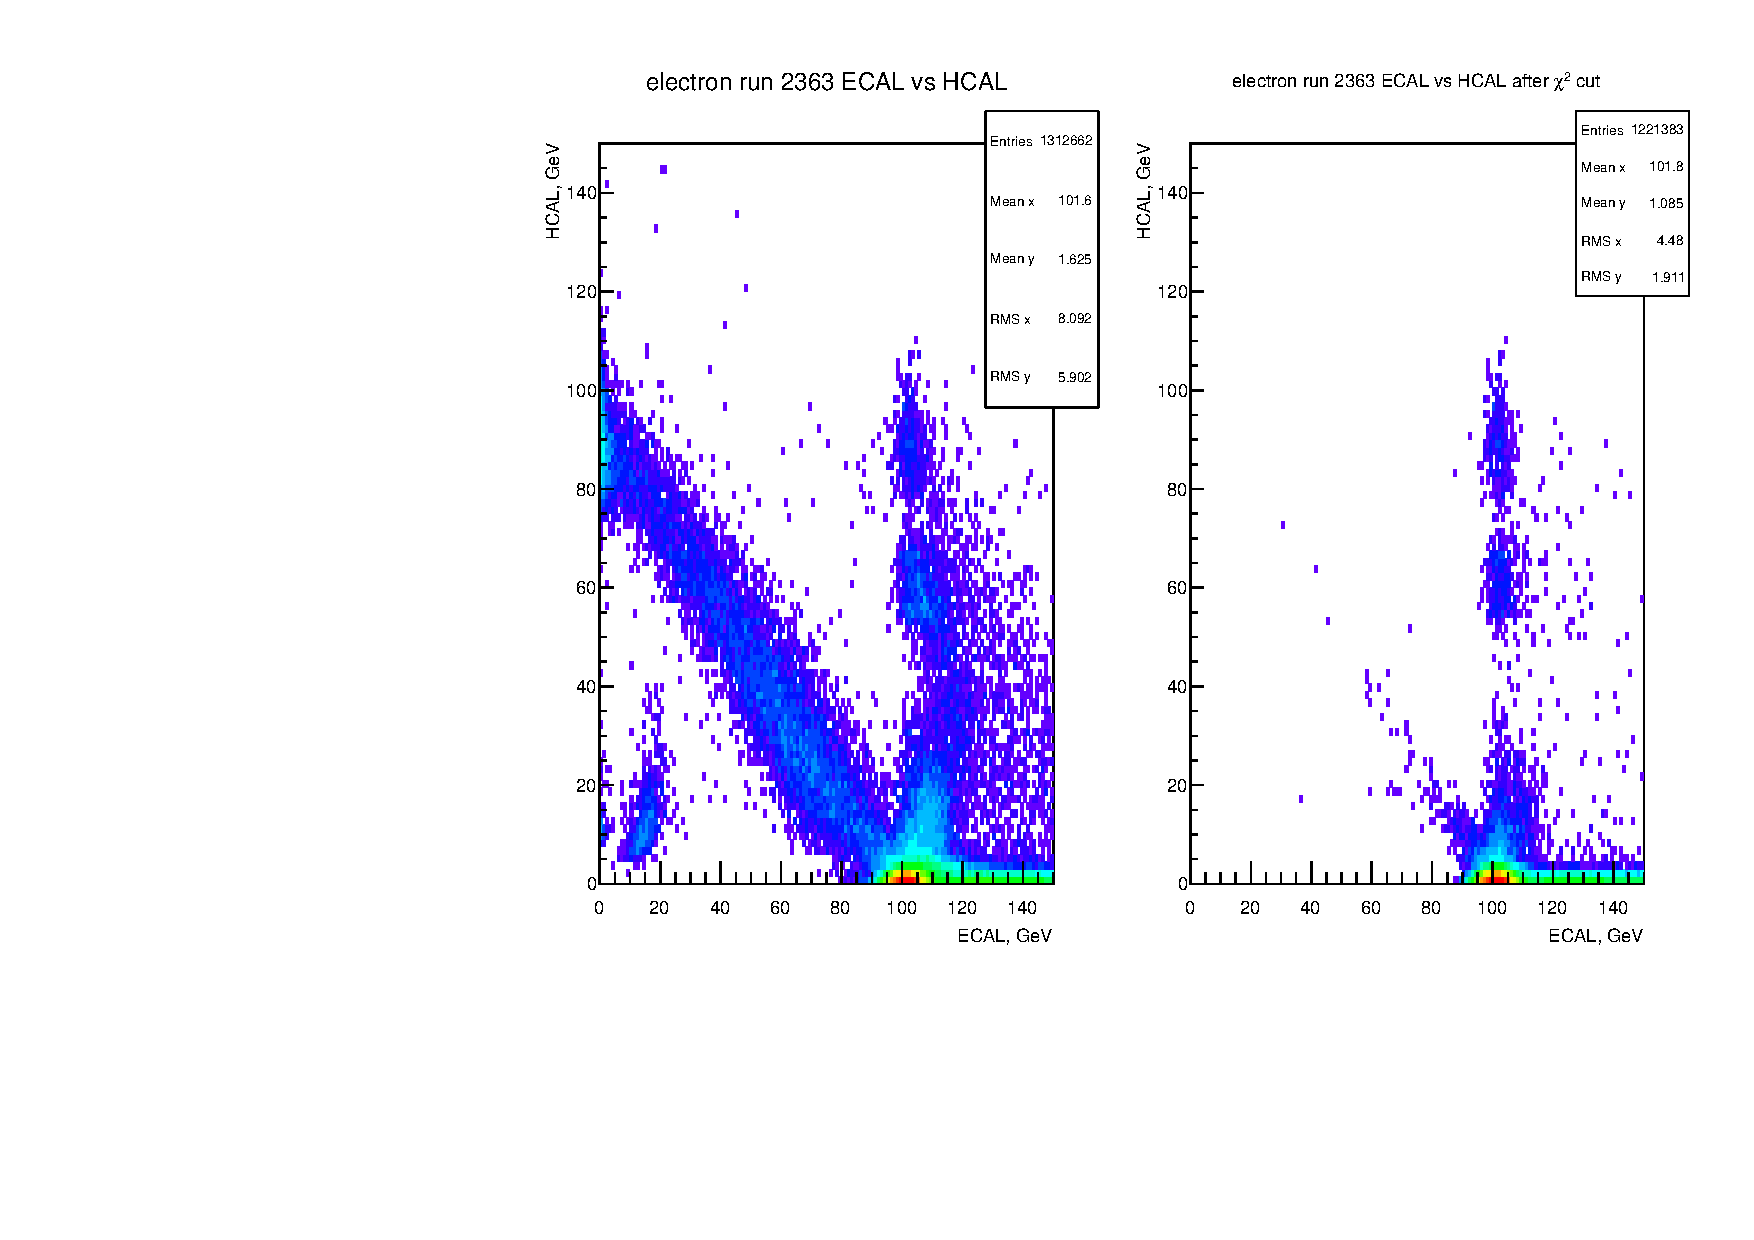
\includegraphics[width=0.95\textwidth,height=0.45\textwidth]{\pdirthree/ehcal_2336_chi.pdf}
    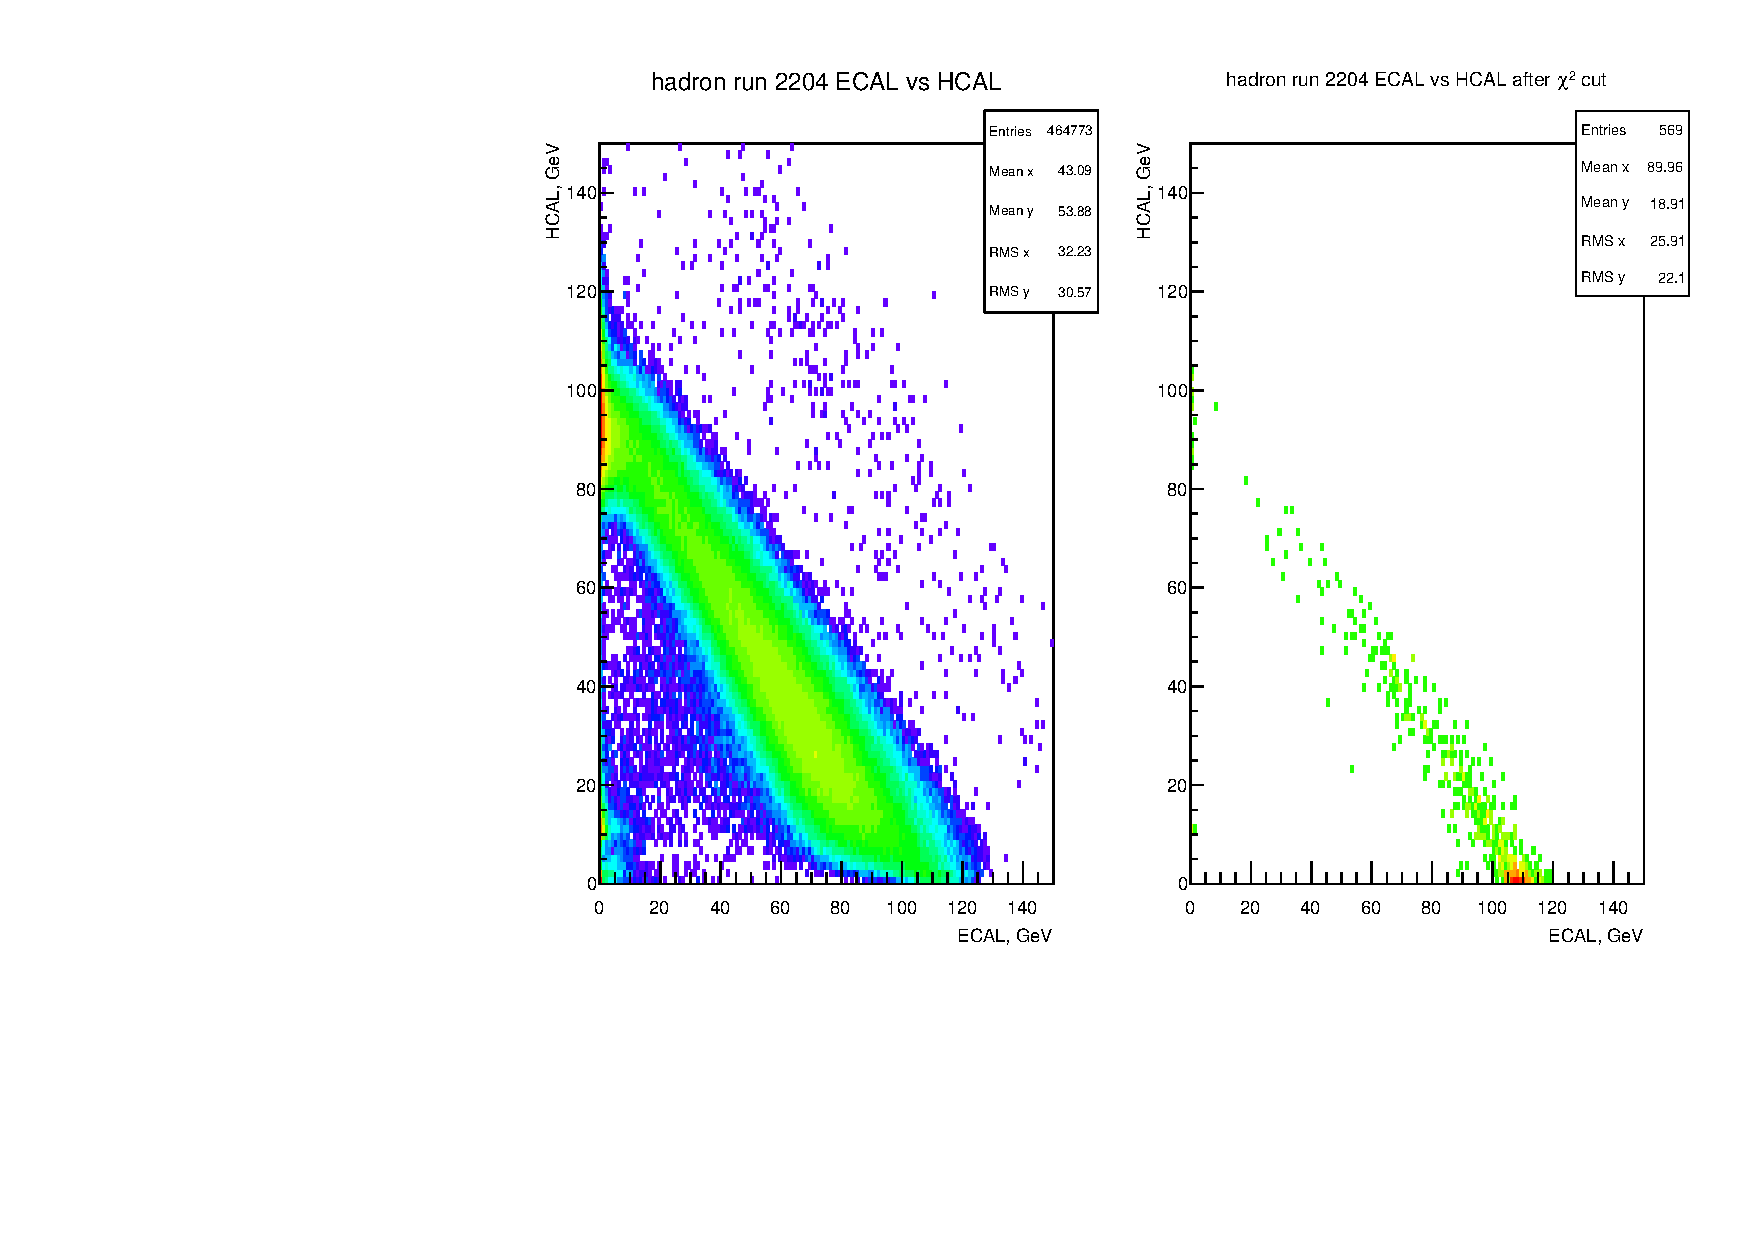
\includegraphics[width=0.95\textwidth,height=0.45\textwidth]{\pdirthree/ehcal_2204_chi.pdf}
    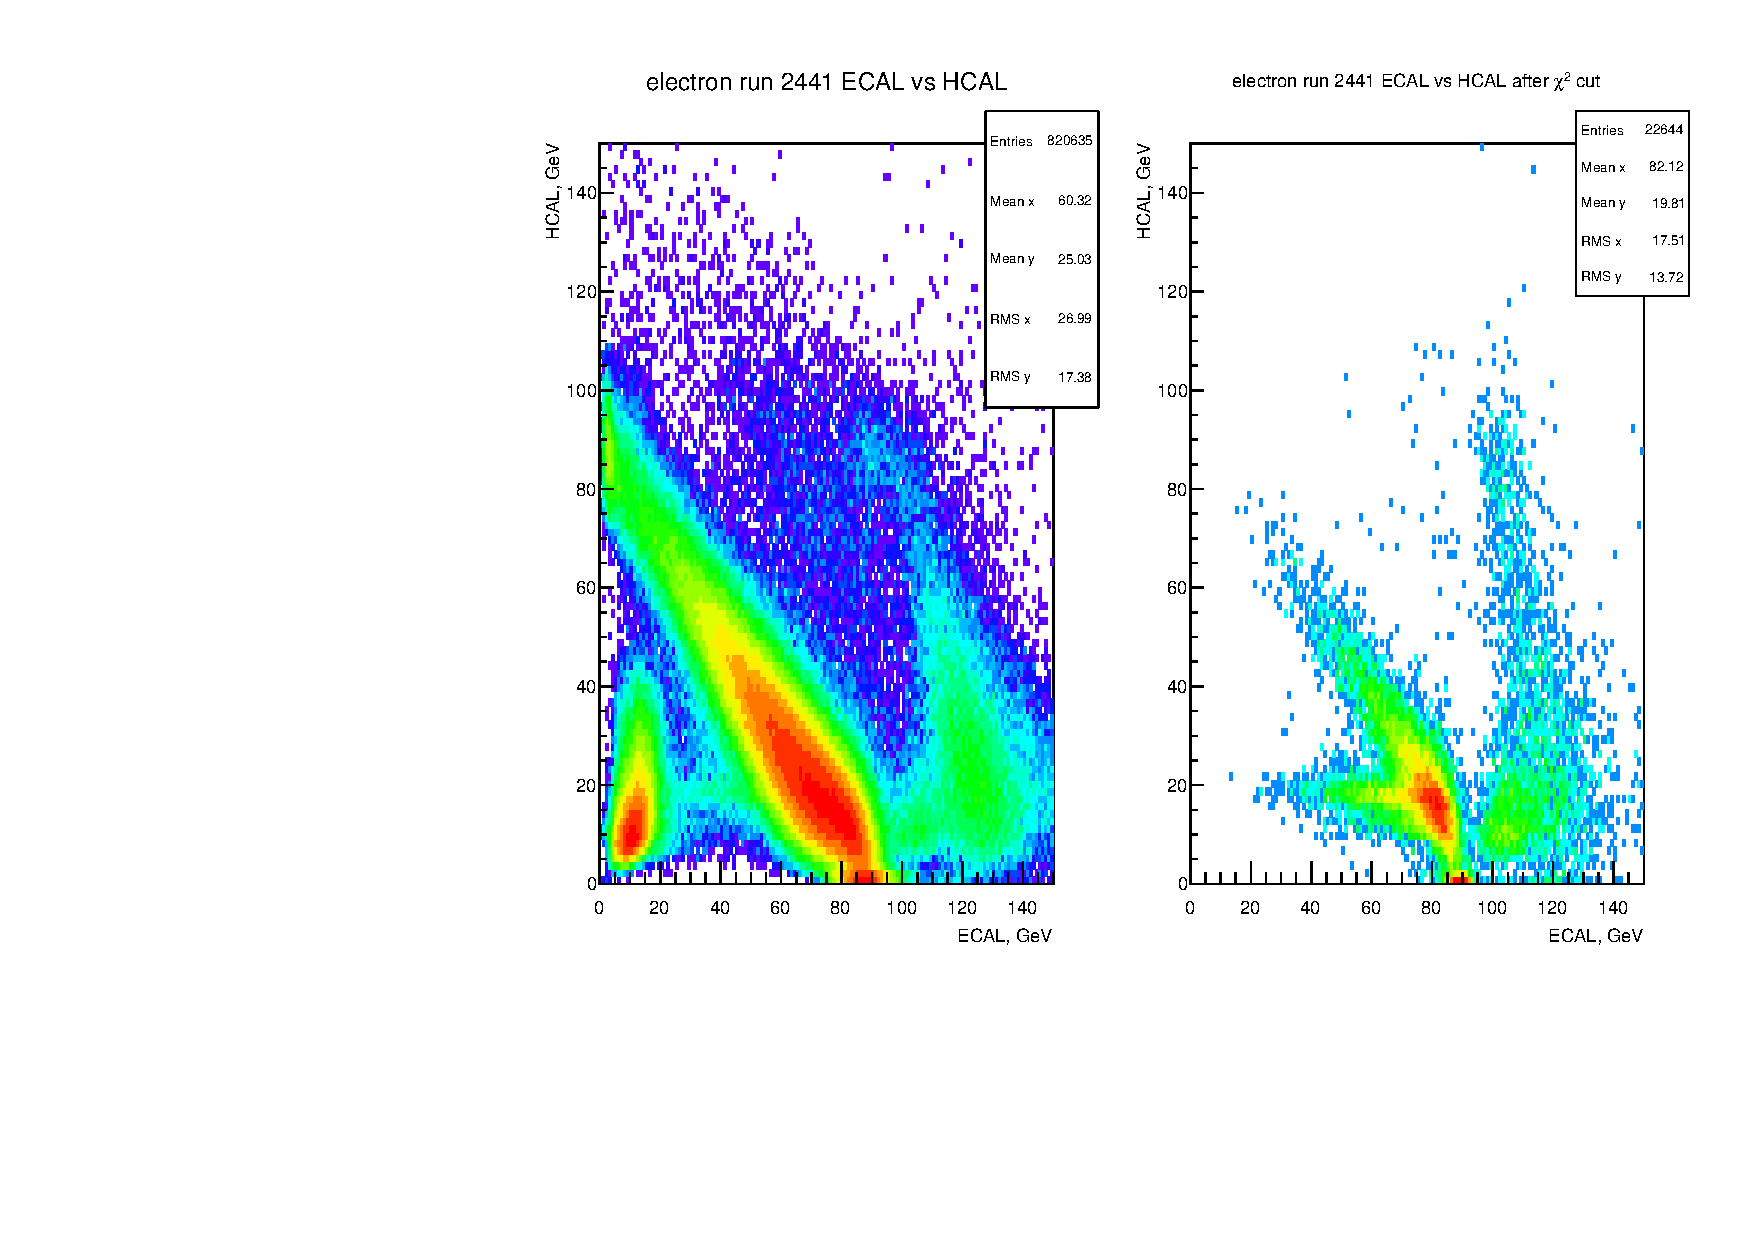
\includegraphics[width=0.95\textwidth,height=0.45\textwidth]{\pdirthree/ehcal_2441_chi.pdf}
  \end{center}
  \caption[ECAL vs HCAL energy deposit after a cut $\chi^2$]{ECAL vs HCAL energy deposit for the total sample (left
    column) and after a cut $\chi^2<2$ (right column) for the
    electron calibration run (top), the hadron calibration run (middle) and the run recorded with physical trigger(bottom).}
  \label{fig:ehcal_test}
\end{figure}
\clearpage

\begin{figure}[h!]
  \begin{center}
    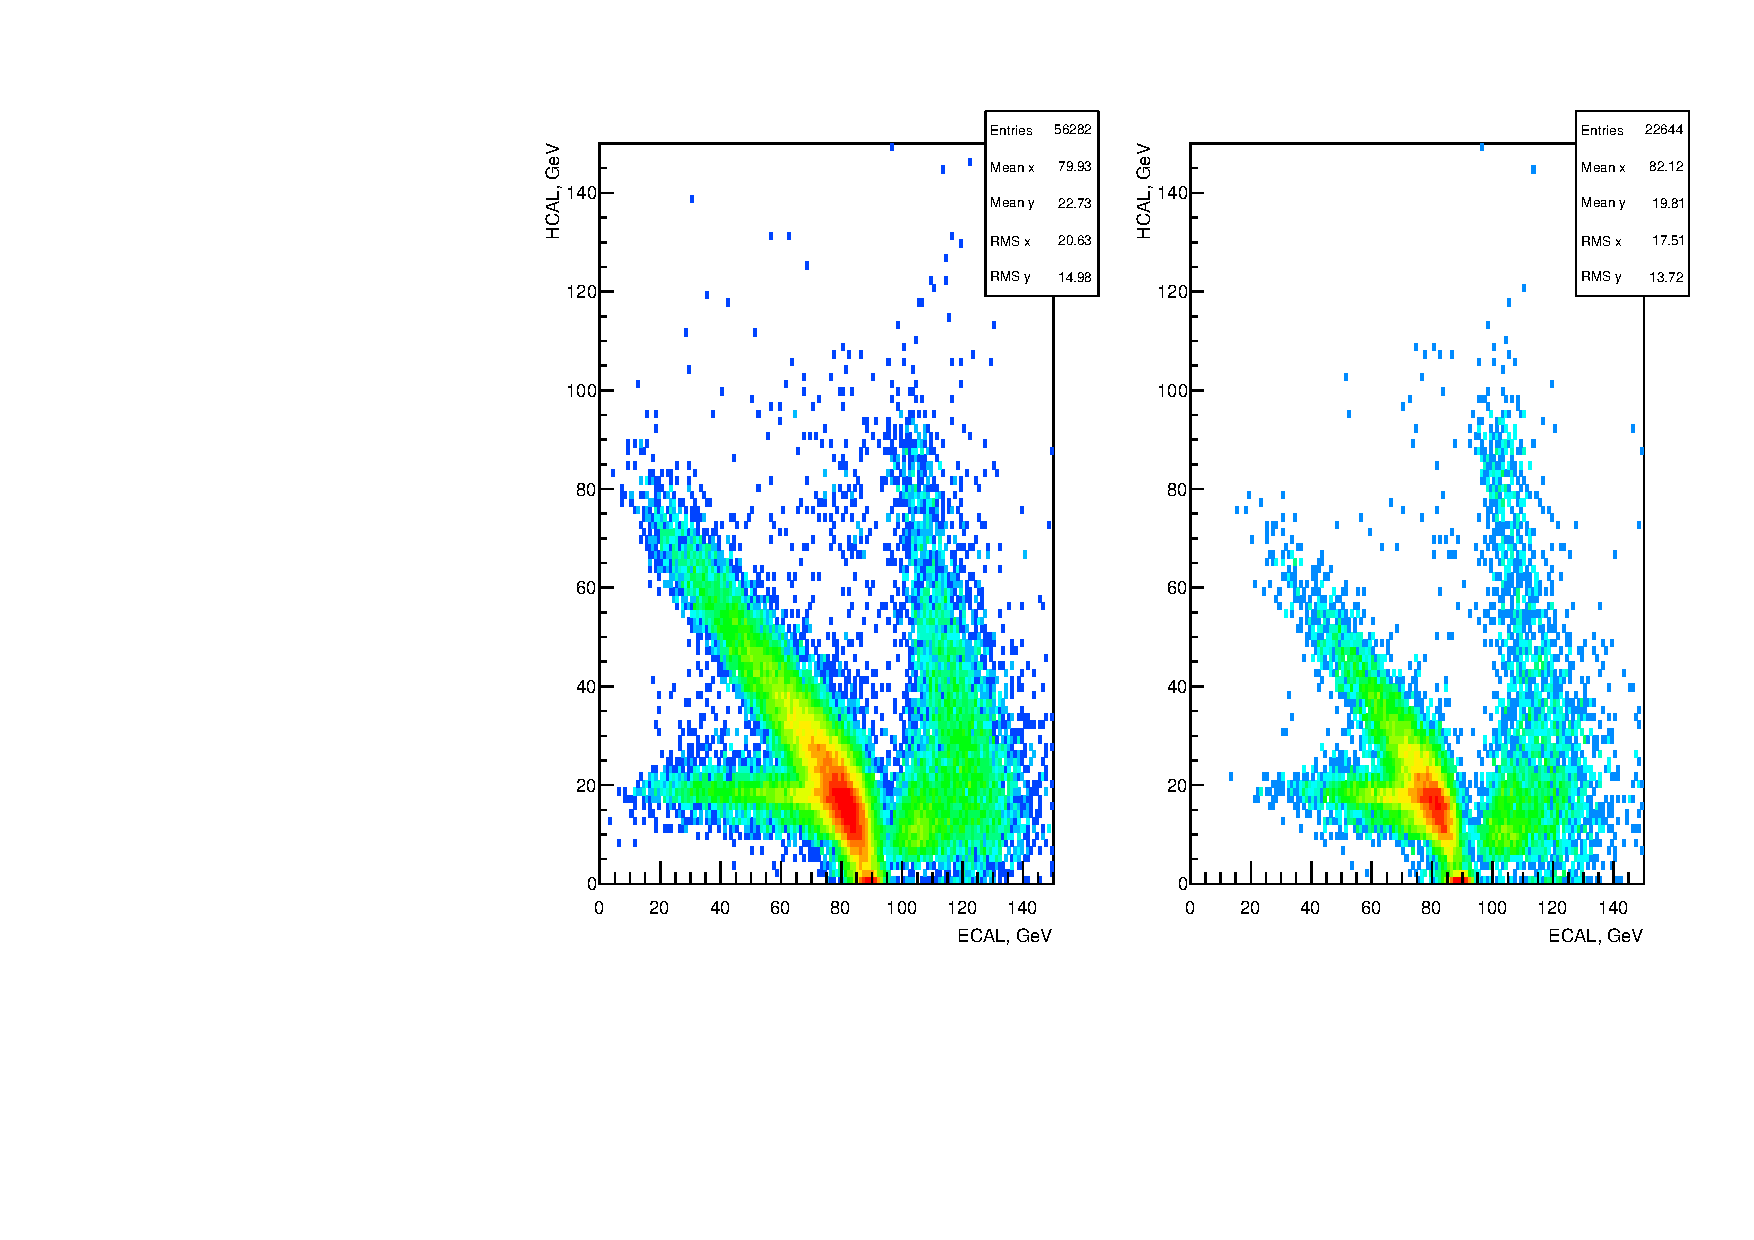
\includegraphics[width=0.95\textwidth,height=0.6\textwidth]{\pdirthree/ehcal_2441_comp.pdf}
  \end{center}
  \caption[ECAL vs HCAL energy deposit after a cut $\chi^2$ for different ECAL configurations]{ECAL vs HCAL after a cut $\chi^2<2$ is applied with the $\chi^2$ calculated with the 9 central cells (left) and for all cells (right).}
  \label{fig:ehcal_comp}
\end{figure}

\iffalse

\section{Comparison with MC}
\label{ch3:sec:mc}
The same profiles described in the section above can be produced using
a 100 GeV electron simulation of the NA64 setup\cite{na64-simulation} and be tested using simulation of $\pi^-$.

We tested qualitatively the effect of a $\chi^{2}$-cut over the
ECAL vs HCAL plots produced for both the MC simulation
and the test runs considered in the previous section. For the
MC-simulation we used the same benchmark cut of the previous section
$\chi^2_{cut}$=2 , while for the data a benchmark cut of
$\chi^2_{cut}$=40 was used to take into account the shift in the
distribution observed.

The bottom plot of Fig.\ref{fig:ehcal_elec} shows that the
contamination of hadron is removed when MC-database is used, so
the hadron shower still produces a significantly larger $\chi^{2}$
compared to the one of an electron shower. The efficiency
observed in the simulation is of ~0.98, slightly larger compared to the data. 
In both simulation and data we can observe that the characteristic
Di-muons events in the range [40,80] GeV in ECAL energy
deposition are accepted.
Fig.\ref{fig:ehcal_hadr} also shows the hadrons to be rejected in both
cases, with a rejection power of $\sim 5\times 10^{-3}$ measured in the
simulation. Also for both simulation and data we can observe that the
events surviving lie mostly in the diagonal $E_{ECAL}$+$E_{HCAL}$= 100
GeV (as could also be observed using a database built from calibration run like in Fig.\ref{fig:ehcal_comp}), while all the events where the shower has large angular spread are rejected.
\\
The main difference between the two plots concerns some events with very low energy deposited in the ECAL that are accepted in the data but not in the simulation. This would suggest that the ECAL cells are subject to some fluctuation that at low energy can sometime mimic the correct electromagnetic-shower signature. As stated in the previous section however for such low energy events the usage of the shower-profile algorithm should be avoided since all the shower will be completely contained in the cell 3x3.\\
% Finally the MC-database was applied to the physical run 2441 always
% with a benchmark cut $\chi^2_{cut}$=40.

\fi


\begin{figure}[h!]
  \begin{center}
    \includegraphics[width=0.95\textwidth,height=0.8\textwidth]{\pdirthree/ehcal_2363_chi_mc_2.pdf}
  \end{center}
  \caption{\textbf{Top}: ECAL vs HCAL before (left plot) and
    after (right plot) a cut
    $\chi^2<2$ in MC simulated 100 GeV electron events. \\
    \textbf{Bottom}: ECAL vs HCAL before (left plot) and after (right
    plot) a cut
    $\chi^2<40$ in the electron run 2363.\\
    The $\chi^2$ was computed using all ECAL cells with a shower
    profile database obtained from a 100 GeV $e^-$ MC-simulation. }
  \label{fig:ehcal_elec}
\end{figure}

\begin{figure}[h!]
  \begin{center}
    \includegraphics[width=0.95\textwidth,height=0.8\textwidth]{\pdirthree/ehcal_2204_chi_mc_2.pdf}
  \end{center}
  \caption{\textbf{Top}: ECAL vs HCAL before(left plot) and
    after(right plot) a cut
    $\chi^2<2$ in MC simulated 100 GeV $\pi^-$ events. \\
    \textbf{Bottom}: ECAL vs HCAL before (left plot) and after (right
    plot) a cut
    $\chi^2<40$ in the hadron run 2204.\\
    The $\chi^2$ was computed using all ECAL cells with a shower
    profile database obtained from a 100 GeV $e^-$ MC-simulation. }
  \label{fig:ehcal_hadr}
\end{figure}

\clearpage
\newpage

\subsection{Study of K$^0_S$ background in visible mode}
\label{ch3:sec:bkg-k0s}

\subsection{Study of neutral punch-through in the Calorimeters}
\label{ch3:sec:bkg-neutrals}

\section{Study of $\gamma + Z \rightarrow \mu^+ \mu^-$ events }
\label{ch3:sec:dimuons}

To validate the MC simulation and the tracking procedure required for this analysis, a pure sample of events containing the rare QED interaction $\emu$ has been studied. This class of events has many similarities to the $\DM$ ones, and they can be easily selected by requiring a double MIP signature in the HCAL modules. This procedure is described in detail in \cite{na64-prd}. The double tracks expected in the decay volume are then used to test the reliability of the tracking procedure in the setup.

To improve the quality of the MC, a realistic beam profile was extracted from the electron calibration runs. Hadrons in the sample were rejected by requiring an energy between 5 MeV and 100 MeV for both SRD counters. The beam profile is then recovered by fitting the XY position recorded by MM3,4 in Fig.\ref{fig:setup-vis-2018} with a 2D Gaussian. The two fits agree within 100 $\mu$m precision for both $\sigma_x \approx 4.13$ mm and $\sigma_y \approx 1.40$ mm. Fig.\ref{fig:dimuon:gemspectra} shows a comparison of the reconstructed hit-position between data and MC in $\emu$ events after the extracted beam profile is used in the simulation.

To further improve the agreement between data and MC several strategies were used. The limited spatial resolution of GEMs was taken into account by applying a smearing of 80 $\mu$m. This number was estimated by checking track residuals after selecting different GEMs triplets for the track reconstruction and comparing the reconstructed hit to the one predicted by the tracking procedure. To reproduce the single planes of the GEM, hits are separated in X-Y projections and knowledge on the original hit combination is no longer assumed. As the minimal hit separation between hits in GEM was conservatively estimated to be 1.75 mm, hits closer than this threshold were merged in the MC. This number was estimated using clusters recorded by the GEM detectors during electron run in 2017. The hits generated in this procedure are used as input for the same reconstruction algorithm used for the data.

The reconstruction chain works as follows:
\begin{enumerate}
\item Track candidates are defined by grouping hits where the angle between first and second GEM pair is smaller than 9 mrad.
\item Those candidates are reconstructed using a Kalman filter implemented with the Genfit library \cite{genfit}.
\item Vertex candidates are generated by grouping tracks pair with no common hits.
\item The exact position of the vertex is obtained by back-propagating the tracks at their point of minimum distance. Only vertices with a distance below 3 mm are considered for the analysis.
\end{enumerate}

\begin{figure}[tbh!]
  \begin{center}
    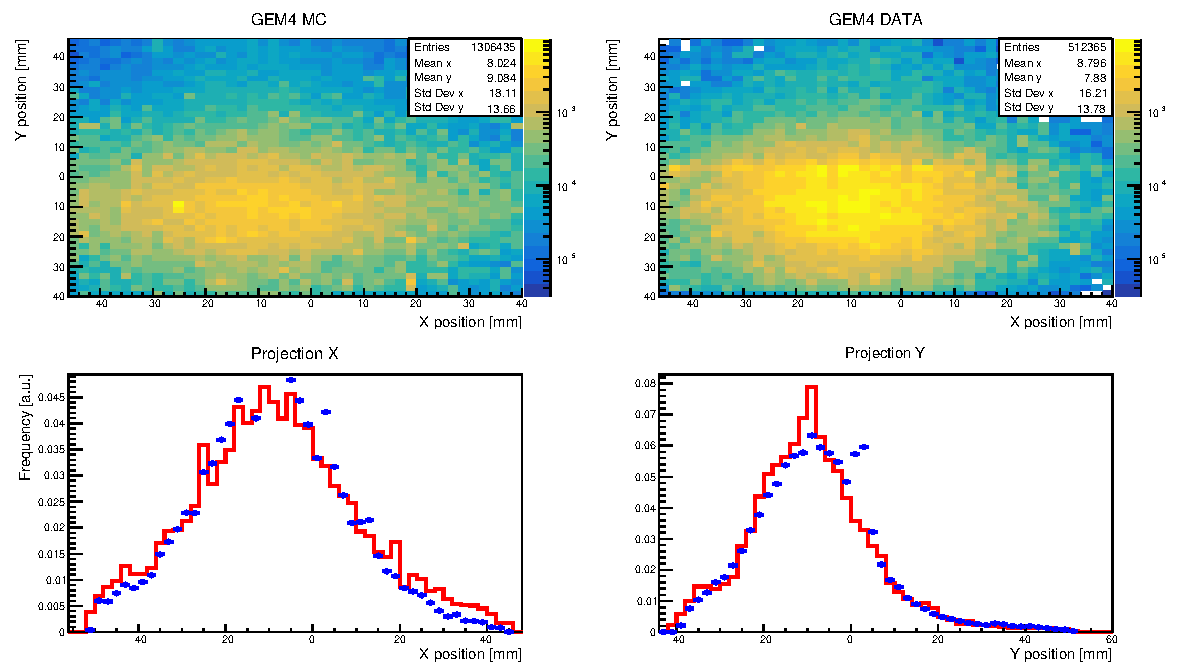
\includegraphics[scale=0.8]{\pdirthree/GEM4_rel.pdf}
  \end{center}

  \caption[Hit position of $\emu$ in GEM MC-DATA]{Hit position recorded in last GEM before ECAL for MC simulated (Red curve) and data (Blue dots) $\emu$ events.}
  \label{fig:dimuon:gemspectra}
\end{figure}
  

A dimuon sample was selected using all events collected during the visible mode 2018 run. The beam quality was improved by requiring a reconstructed momentum in the range between 140 and 160 GeV. The $\emu$ events leave a double-MIP signature in each HCAL module, thus a cut 2 GeV$<$ E$_{hcal} <$ 6.35 GeV is applied for the selection. Since an hardware trigger which selects only events with missing energy in the WCAL is used during the data taking, an additional cut $E_{WCAL} < 90$ GeV is applied to consider only such events in both simulation and data. This cut also selects a sample with kinematics closer to the one expected from a $\DM$ candidate. This makes the comparison with the MC more significant for our search. Scintillator counters also need to be compatible with a $\mu^+ \mu^-$ in the decay volume: an energy deposited of at least 1 MIP is required in the scintillator (S4) downstream the WCAL and at least 1.8 MIP in the Veto behind the ECAL. The less stringent cut on S4 is justified by its limited transverse dimension which makes it not suitable for a precise energy measurement.

Although these cuts mainly select dimuon generated from $e^-$ primaries, a contribution is also expected from the hadron contamination. The physical trigger employed in the experiment further increases such contribution, as the requirement of low energy deposit in the WCAL bias the beam composition to particles with high penetration power. To solve this issue, a cut on the SRD detector and on the WCAL pre-shower are used. These cuts are expected to reject hadrons and muons at a level $<10^{-5}$.

To cross-check that the contamination is correctly removed, an independent method based on the beam profile shape is used. The beam profile significantly differs between electrons and hadrons as the H4 beamline is tuned for selecting electrons in our search. Both profiles are recovered from the data using a calibration run of electron/hadron respectively. Using a  $\chi^2$-test the ratio between the two is estimated by mixing the two templates until the best agreement with the measured beam profile is reached. The result is summarized in Fig.\ref{fig:dimuon:profile}: the beam profile of dimuon-selection events is compared before and after the SRD criteria is applied. The fit shows a contamination of roughly 50\% in the original sample. After the cut the beam profile converges to the templates obtained in the $e^-$ calibration runs.

\begin{figure}[tbh!]
  \begin{center}
    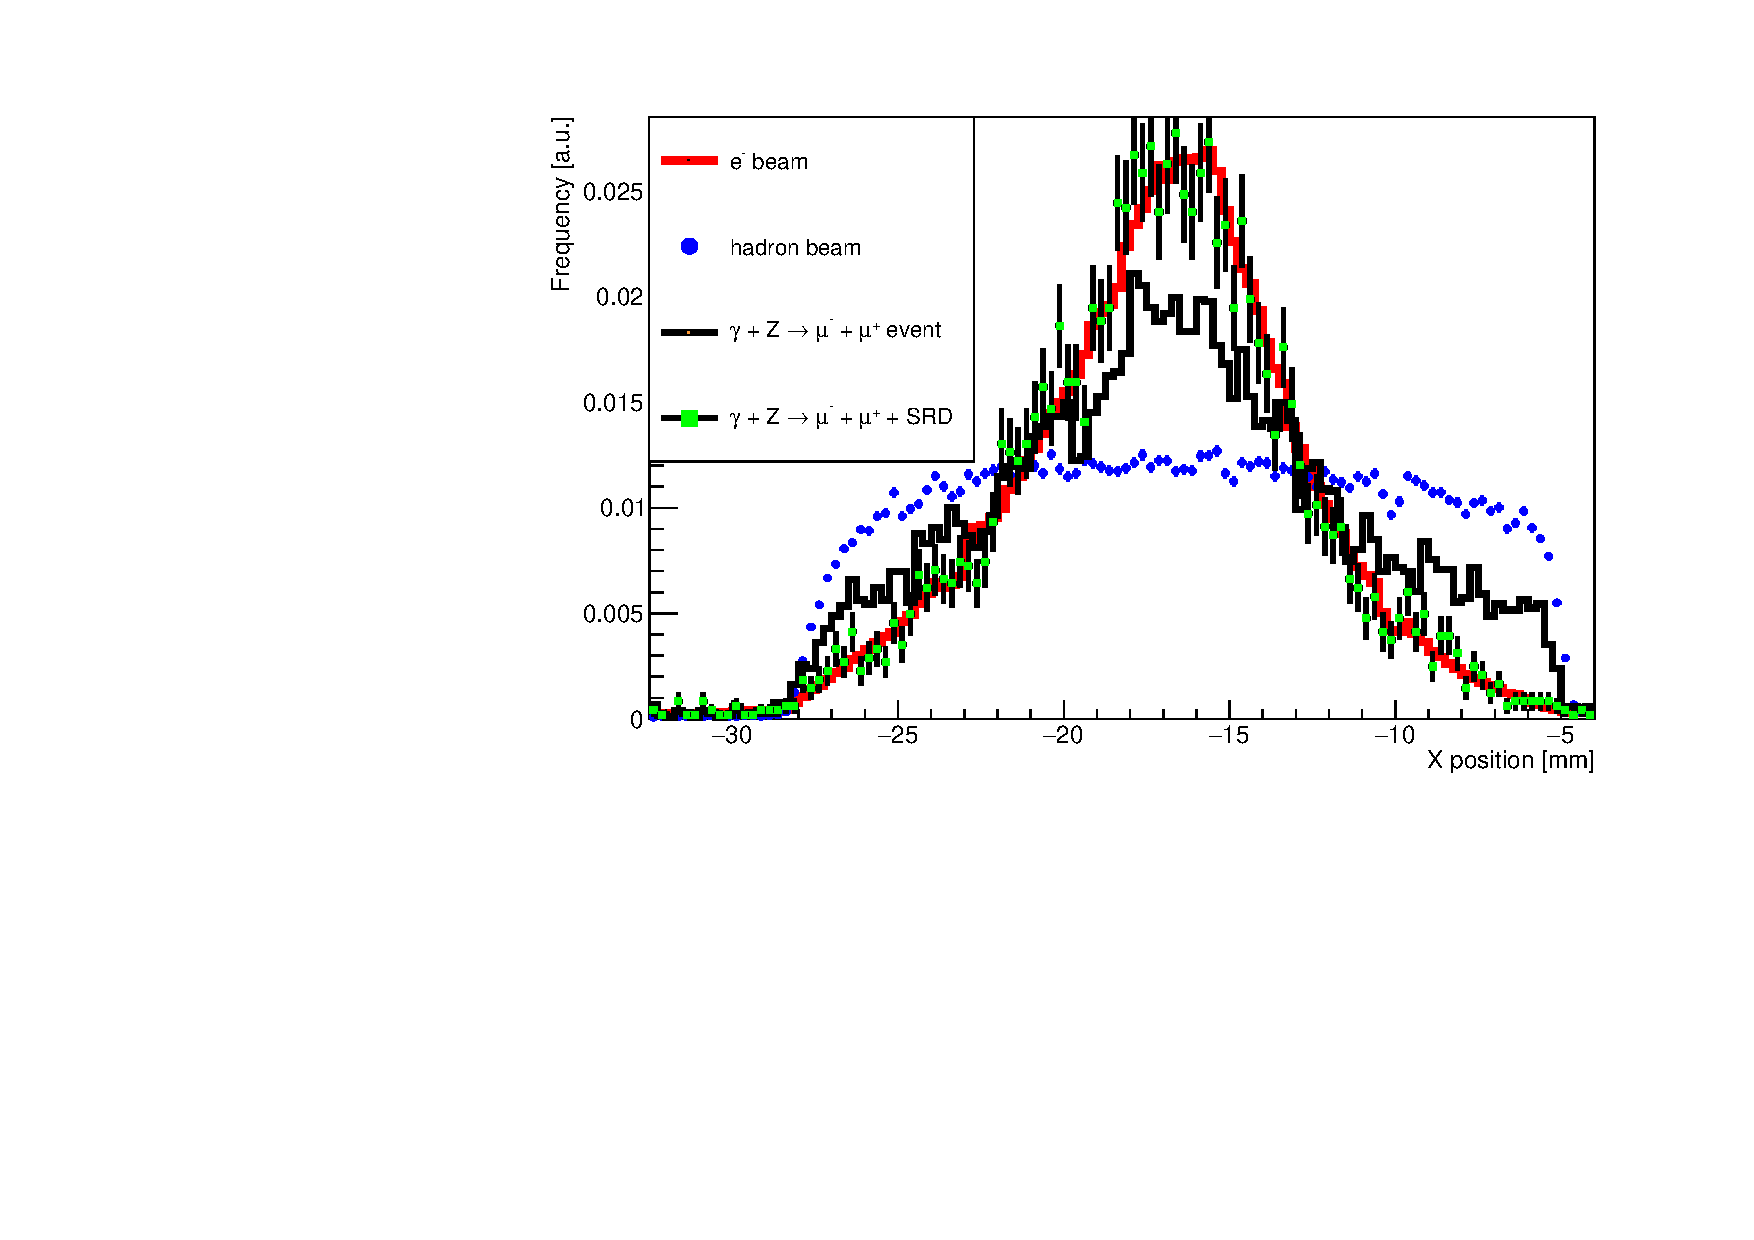
\includegraphics[scale=0.8]{\pdirthree/beamspot.pdf}
  \end{center}
  \caption[Beam profile with different cuts]{Beam profile recorded by the first Micromegas module upstream for hadron calibration run (blue dots), electron calibration run (red line), events selected with dimuons cuts from data collected with the physical trigger (black line) and those same events after SRD cut is applied (green square). Fits using the templates obtained from the calibration run show a level of contamination of $\sim$50\% in the dimuon sample. The contamination is completely removed after the SRD cut is applied.}
  \label{fig:dimuon:profile}
\end{figure}

%\subsection{Vertex and angle reconstruction}
%\label{ch3:sec:dimuons-reco}

\subsection{Signal yield correction}
\label{ch3:sec:dimuons-sig-corr}

To show that there are no significant differences in the tracking procedure between simulation and data the energy deposited in the WCAL was used as a figure of merit. If the tracking procedure affects differently data and MC, one would expect the agreement between the two distributions to diverge after cuts based on vertex reconstruction. Following the procedure described above, a number of vertex candidates are selected for the comparison. As the interaction $\emu$ will have their vertex inside the WCAL, only vertices compatible with this assumption are selected for the comparison. In practice, a vertex is accepted if its position lies within 3$\sigma$ of the expected WCAL position, where $\sigma$ was fitted using a Gaussian from the distribution of $\mu^- \mu^+$ pairs selected from the simulation. After the selection criteria, the energy deposited in the WCAL is compared between simulation and data for each event left (see Fig.\ref{fig:dimuon_en}). The energy deposit for data and simulation is in excellent agreement, proving that the tracking cuts do not bias the original sample.

\begin{figure}[tbh!]
  \begin{center}
    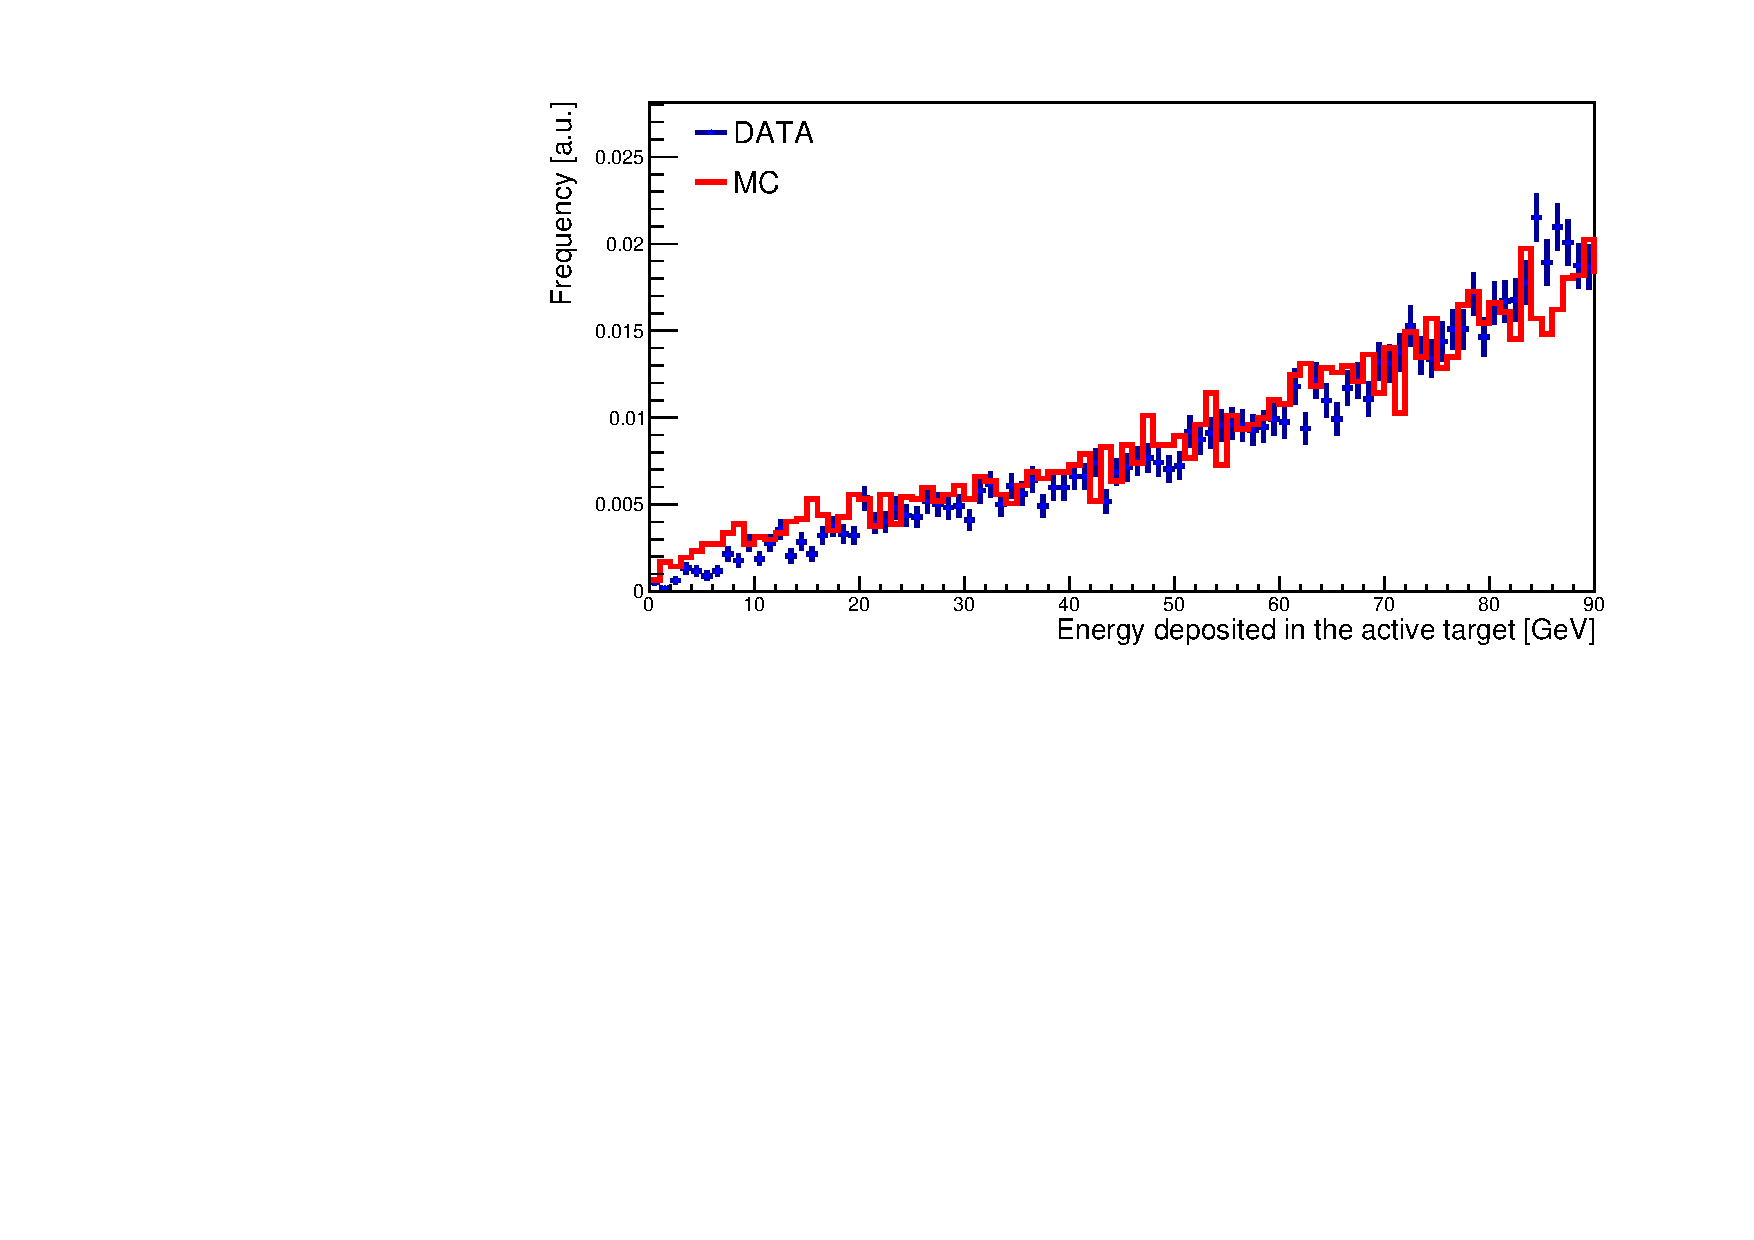
\includegraphics[scale=0.8]{\pdirthree/dimuon_en.pdf}    
  \end{center}
  \caption[$\emu$ MC-DATA comparison]{Energy deposit in the active dump (WCAL) after all selection criteria are applied in $\emu$ event. Data are drawn with blue dots, simulation is plotted with a red line. }
  \label{fig:dimuon_en}
\end{figure}

A lower efficiency is observed in the data compared to the Monte Carlo after applying the selection. The reasons for this are inefficiency of the GEM modules, fail of clusterization in some events and differences in the tracking procedure due to the simplifications used in the MC. The cuts applied to the sample are divided into four steps. First, at least two hits per GEM are required in the decay volume as a minimal condition for tracking. After that, events with a GEM module recording more than 5 hits are rejected as incompatible with a single $\emu$ vertex. The MC predicts 68\% of $\mu^+ \mu^-$ pair after these two cuts. This low acceptance is caused by the GEMs position optimized to resolve very close hits coming from the decay of $\DM$. These selection criteria do not depend on the track-fitting procedure but instead rely on the clusterization performed and the efficiency of the trackers. Tracking procedure is then applied to the events that survived the two first requirements. The reconstructed vertex position is required to be compatible with a vertex inside the dump. The number of events surviving the last requirement  is slightly smaller in the data. The disagreement between the ratio of good vertices reconstructed inside the decay volume is $<$1\%. A total factor of 0.77 is estimated as ratio between data and MC. This factor is used to correct the 2018 signal yield. A summary of the efficiency can be found in Table \ref{tab:dimuon:efficiencies}.

\begin{center}
\begin{table}
  %\centering
  \begin{tabular}{|l|c|c|c|}
    \hline
    cut & efficiency MC & efficiency Data & MC / DATA \\
    \hline
    \textbf{Hit} & & &\\
    \hline
    hits per GEM $\geq$ 2 & 0.68$\pm$0.1 & 0.58$\pm$0.1 & 0.85$\pm$0.1 \\
    hits per GEM $\leq$ 5 & 0.68$\pm$0.1 & 0.55$\pm$0.1 & 0.80$\pm$0.1 \\
    \hline
    \textbf{tracking} & & &\\
    \hline
    Vertex distance $\leq$ 3 mm & 0.63$\pm$0.1 & 0.49$\pm$0.1 & 0.77$\pm$0.1  \\
    Vertex in decay volume & 0.62$\pm$0.1 & 0.48$\pm$0.1 & \textbf{0.77$\pm$0.1}\\
    \hline
    
  \end{tabular}
  \caption[MC/DATA for the tracking procedure and vertex reconstruction]{Efficiency of cuts based on tracking criteria for a clean sample of simulated $\emu$ and dimuon selected from 2018 data. The efficiency presented in the table are cumulative, with the first cut applied being the one in the first row. First two cuts are based exclusively on information coming from the single GEM modules. Last two cuts are based on the tracking procedure.}
  \label{tab:dimuon:efficiencies}
\end{table}
\end{center}

\section{Selection criteria}
\label{ch3:sec:selection-criteria}

\subsection{Invisible mode}
\label{ch3:sec:selection-criteria-invis}

\subsection{Visible mode}
\label{ch3:sec:selection-criteria-vis}

\subsubsection{Analysis using Veto at the end of the dump}
\label{ch3:sec:vis-mode-veto}

\subsubsection{Mixed approach using tracking and Veto}
\label{ch3:sec:vis-mode-tracking}


The published analysis using the data collected in 2018 \cite{Banerjee:2019hmi} was based exclusively on the calorimeters and counters as described in Sec.\ref{ch2:sec:vismode}. The trackers after the decay volume were not used for the signal discrimination. Here we present a novel method which exploits them providing a boost in the signal yields while maintaining the background under control. Even though this analysis is not sensitive when the decay length of the $\DM$ is significantly smaller than the dimension of the dump, it has the advantage of being complementary to the calorimeter analysis. Moreover, it is a very important proof of principle to demonstrate the power of our tracking procedure.

While in a first approximation the $\DM$ is produced in the first few layers of the WCAL, it can also originate at a later stage of the em-shower. These events, which are typically rejected in the calorimeter analysis, are instead accepted in the new analysis presented here. First, an initial sample is selected in the same way described in Sec.\ref{ch2:sec:vismode} and detailed in \cite{Banerjee:2019hmi}. The final discrimination in the calorimeter analysis is based on the counter W2 placed at the end of the dump to reject the charged punch-through from the em-shower. This last cut is efficient if the $\DM$ is produced in the first few layers of the WCAL, but typically reject the event if the $\DM$ is produced at a later stage of the em-shower. The reason is that these events are accompanied by a long longitudinal development of the em-shower that leaves an energy deposit larger than the typical energy cut accepted in the calorimeter analysis. On the other hand, the low energy of the produced $\DM$ implies a larger angle between the decay products that can be resolved by the trackers. Combining these two concepts, one can see that the signal yield is characterized by two different topologies that can be easily distinguished by looking at the energy deposited in the ECAL (see Fig.\ref{fig:combined-analysis}).

Using this distinction, we divide all events that passed the initial selection criteria in two topologies based on the total energy deposited in the ECAL. The exact value of this threshold was selected to maximize the signal yield. The optimal value has a small dependence on the $\DM$ mass and coupling. A simple threshold of 75 GeV amounting to half of the initial beam energy was found to be robust for most of the interesting signal scenario. After the topology is decided, a final set of cuts is applied to discriminate between signal and background. In the case of high energy $\DM$, trackers do not have the capability of discriminate between single hits. An energy deposit smaller than 0.8 MIP is required in W2, and the presence of a decay after the dump is assessed by asking S4 to have an energy deposited larger than 1.5 MIP. On the other hand, if the energy deposited in the ECAL is smaller than 75 GeV, trackers are used instead as final discriminator. Two tracks in the decay volume are required with a reconstructed vertex within 3$\sigma$ from the WCAL and an angle smaller than 3 mrad. This different treatment leads to an increased efficiency to $\DM$ produced at a late stage of the shower as shown in Fig.\ref{fig:combined-analysis}. However, the smaller energy of the $\DM$ produced in this way has the effect of reducing the probability of the particle escaping the dump. For large coupling $\epsilon$ this suppression can be more than 2 orders of magnitude, making the boost of signal yield negligible. A summary of this boost for various interesting $\DM$ and $A'$ scenario is illustrated in Table \ref{tab:dm:efftable}. The values reported consider also a conservative correction factor of 0.77$\pm$0.1 that takes into account inefficiencies of the detectors and the reconstruction algorithm. This factor was evaluated using a data-driven method precisely outlined in Sec.\ref{ch3:sec:dimuons}. The conclusion of this study is that in the current setup trackers information do not improve the limit on the $\DM$ parameter space. This is because the boost in signal yield becomes negligible for $\epsilon \sim 6 \times 10^{-4}$, a value which is already excluded with 90\% confidence by our previous analysis.

\begin{figure}[tbh!]
  \centering
  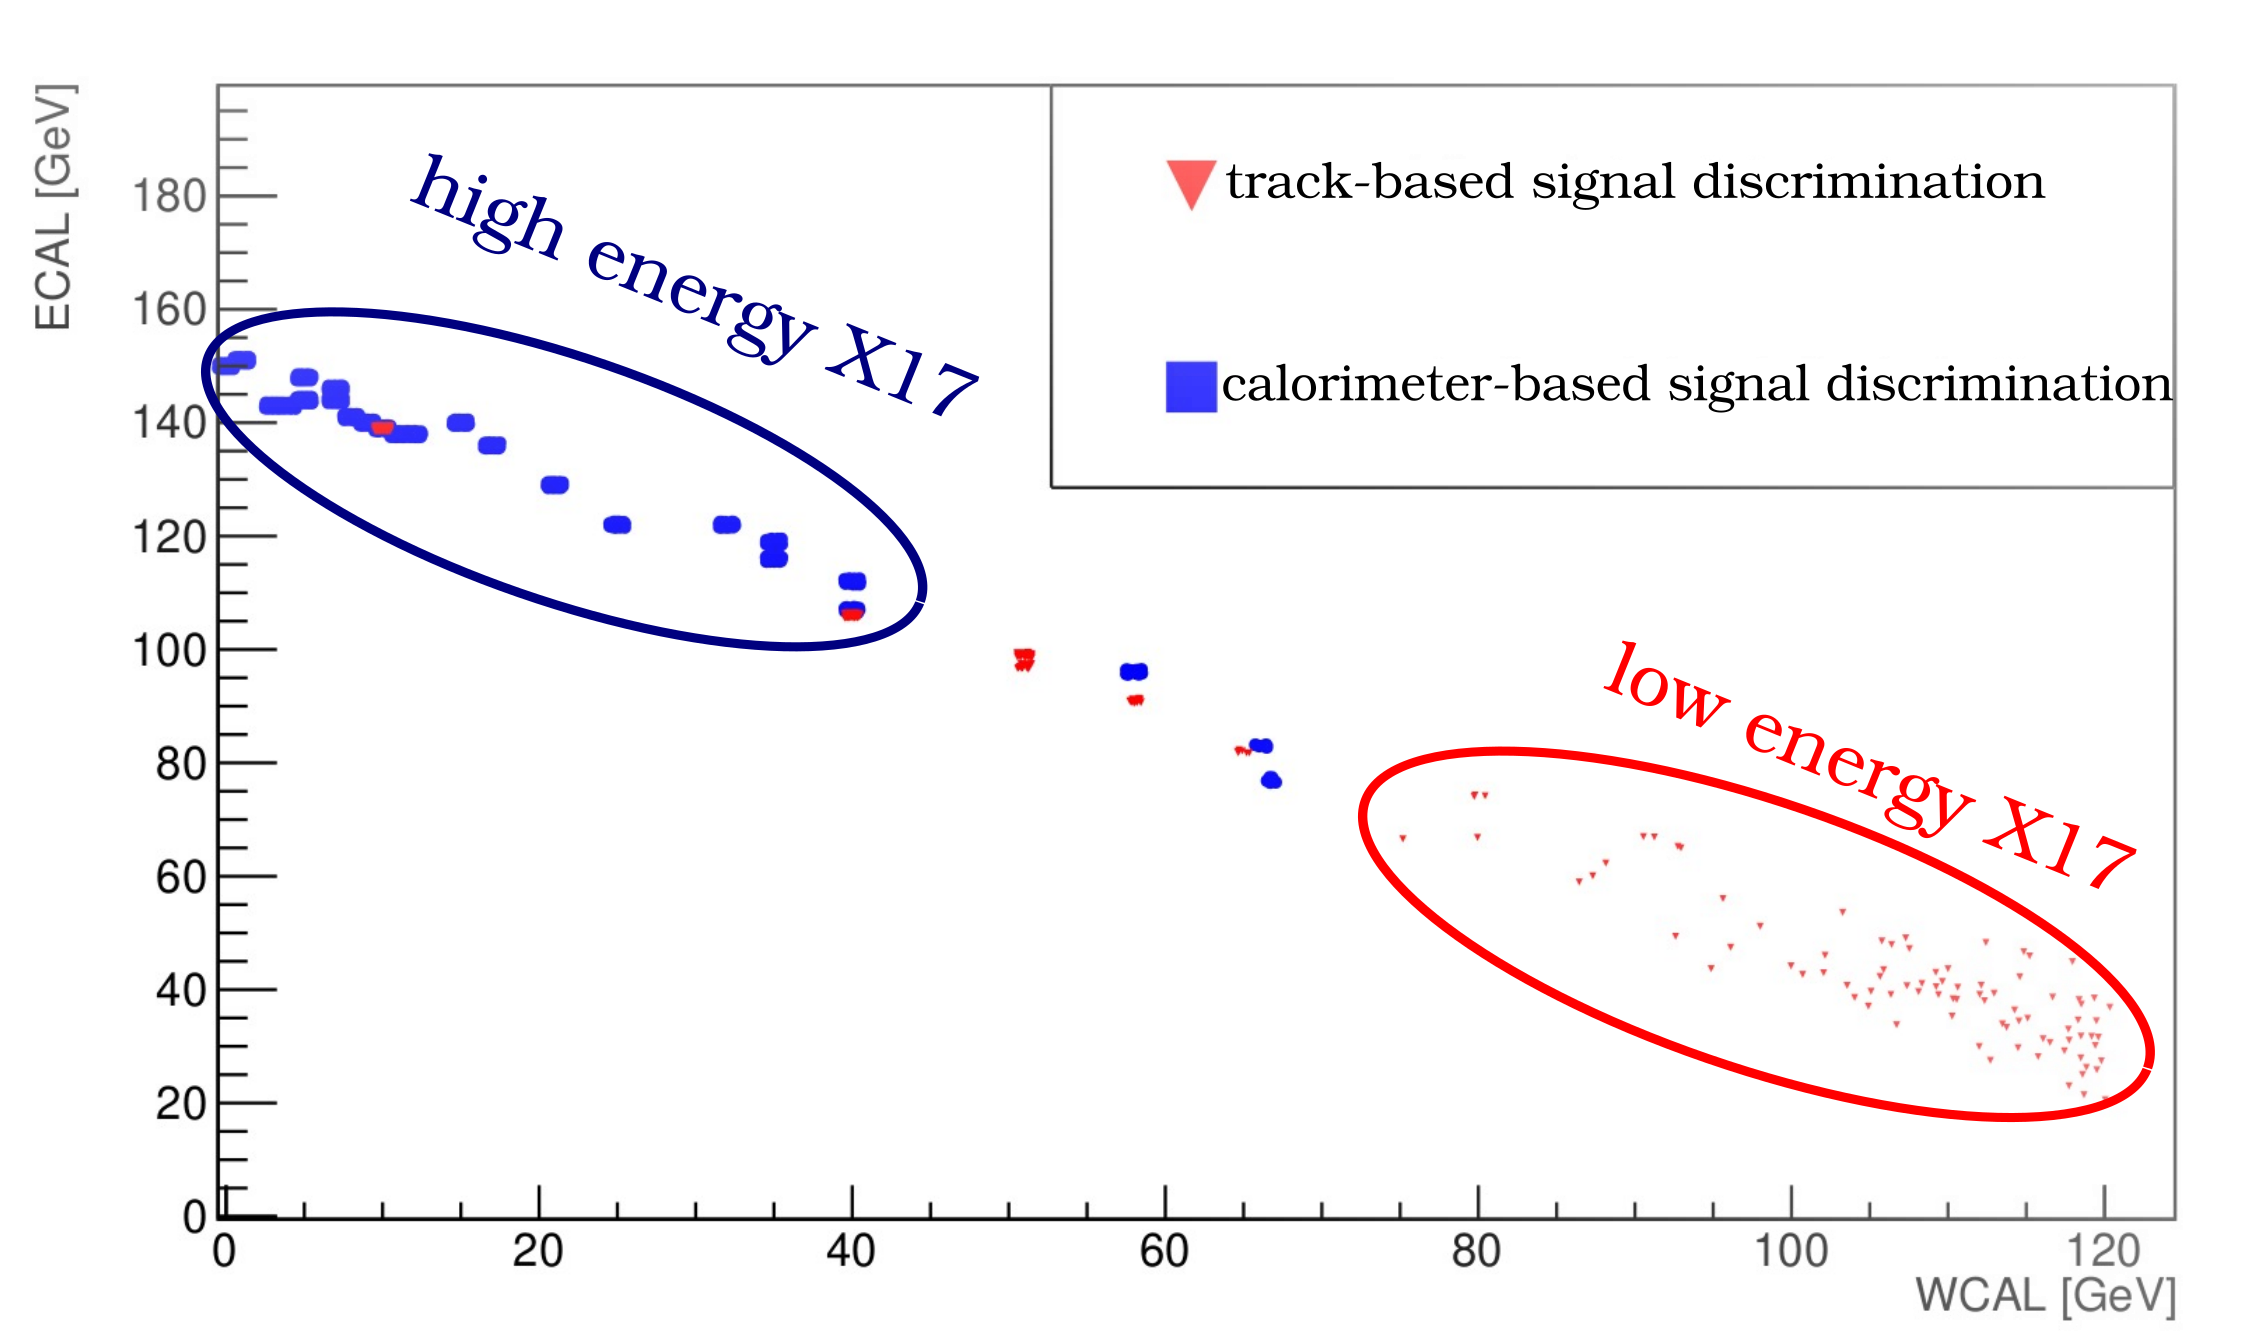
\includegraphics[scale=0.9]{\pdirthree/X17-separation-v2.png}
  \caption[Comparison of selected $\DM$ between calorimeter and tracking analysis]{$\DM$ simulated in the visible mode 2018 setup. Two different cuts are used to discriminate between two $\DM$ topologies. The first one is based on angle cut and vertex position using information from the 4 GEM stations installed in the decay volume and is very efficient on the $\DM$ produced at low energy (red triangle). The second one relies on the Veto placed at the end of the dump and is more efficient for the high energy population (blue square).}
  \label{fig:combined-analysis}
\end{figure}

\begin{center}
\begin{table}
  \centering
  \begin{tabular}{llr}
    \hline
    M$_{A'}$ [GeV]& $\epsilon$ & N$^{new}_{A'}$ / N$^{old}_{A'}$ \\    
    \hline
    0.005  & 0.004    & 1   \\    
    0.01   & 0.0015   & 1   \\    
    0.01   & 0.003    & 1   \\    
    0.0167 & 0.0001   & 1.22\\
    0.0167 & 0.00018  & 1.2 \\    
    0.0167 & 0.000316 & 1.2 \\
    0.0167 & 0.0006   & 1.01\\
    0.0167 & 0.0007   & 1   \\
    0.022  & 0.000316 & 1.22\\
    \hline    
  \end{tabular}
  \caption[ratio between signal events observed in tracker-analysis compared to calorimeter-only analysis]{N$^{new}_{A'}$ / N$^{old}_{A'}$ ratio between signal events observed in tracker-analysis compared to calorimeter-only analysis. The new analysis uses cuts based on GEM tracking detectors if the energy detected by the downstream ECAL is below 75 GeV.}
  \label{tab:dm:efftable}
\end{table}
\end{center}



%%% Local Variables:
%%% mode: latex
%%% TeX-master: "../PhDthesis"
%%% End:
